%% paper04 — 独立小论文稿(中文)
%% 模板: ACM acmart manuscript。正文已与旧 NOSR/HMACSP 叙事脱钩,仅保留版式骨架。
%% 编译: XeLaTeX(必须;见下方 ctex 说明)。
%%
\documentclass[manuscript,screen,review]{acmart}

%% ===================== 中文支持 =====================
%% scheme=plain: 只接管中文字体与断行,不改写 acmart 的章节名。
%% fontset=windows: 本机宋体/黑体; Overleaf/Linux 可改为 fontset=fandol。
\usepackage[UTF8,scheme=plain,fontset=windows]{ctex}

\usepackage{algorithm}
\usepackage{algorithmicx}
\usepackage{algpseudocode}
\usepackage{pifont}
\usepackage{makecell}
\providecommand{\checkmark}{\ding{51}}
\newcommand{\cmark}{\ding{51}}
\newcommand{\xmark}{\ding{55}}
\usepackage{threeparttable}
\usepackage{tikz}
\usetikzlibrary{positioning,arrows.meta,calc,shapes,shadows}
\usepackage{xcolor}
\usepackage{amsmath}
\usepackage{bm}
\DeclareMathOperator*{\argmin}{arg\,min}
\DeclareMathOperator*{\argmax}{arg\,max}
\usepackage{multirow}
\usepackage{enumitem}
\usepackage{booktabs}
\usepackage{graphicx}
\setlength{\headheight}{20.48303pt}
\renewcommand{\topfraction}{0.85}
\renewcommand{\bottomfraction}{0.6}
\renewcommand{\textfraction}{0.1}
\renewcommand{\floatpagefraction}{0.75}

%% scheme=plain 不改浮动体名称,与 paper01 中文稿对齐。
\renewcommand{\figurename}{图}
\renewcommand{\tablename}{表}
\floatname{algorithm}{算法}
\renewcommand{\proofname}{证明}

%% 机制缩写:主语是闭包,不是「修复框架」
\providecommand{\STRC}{\textsc{STRC}}
%% B13 删去 \TBD:全稿 0 处引用,待填项一律用 <待填:...> 明文标记,便于自检抓取。

%% =====================================================================
%% 主结果数字的单一来源。
%%
%% 全部由 STRC/tools/paper_numbers.py 从 STRC/experiments/expanded/*.csv 打印,
%% 数据由 `py -m tools.expand_batch` 生成(默认 5 算例 x 10 种子)。
%% 正文一律用宏,不写字面量;改数只改这里,并同步跑一遍上述两条命令核对。
%%
%% 注释与 CSV 列名沿用旧臂名,与正文方法名对应为:
%%   R1 = AOR,R2 = STRC,R0+ = GR,RA = UR;RS、RD 不变。
%%
%% !! 2026-08-16 由 3x5=15 对扩到 5x10=50 对。旧稿所有 /15 结果一律作废。
%%
%% !! 2026-08-16(二次):E2b 由 24/50 变为 50/50。这不是换了算例,而是修掉了
%% !! 一处实现与定义的错配。释放集是一个**预约**集合,而 replay_reroute 原先
%% !! 按**工序**判定是否重路(两段中任一段进闭包就整道重规划)。于是当只有满载
%% !! 段进闭包时,同工序的空载段也被改写,而它的 task 并不在释放集里,遂被记为
%% !! 外侧漂移。26 个失败格上的 84 条漂移预约无一例外都是这种同工序空载段,
%% !! 其中 71 条(85%)在 t_now 之前就已执行完毕——改写它同时违反假设 A2。
%% !! 改为按段判定后漂移归零。据此 prop:outside 的前提 (iii) 才真正被满足,
%% !! 此前的 24/50 测的是实现缺陷,不是边集的物理覆盖度。
%% =====================================================================
\newcommand{\NInst}{5}
\newcommand{\NSeeds}{10}
\newcommand{\NPairs}{50}
%% E1/E3:两项都是满分,写成 \NPairs/\NPairs 以免手抄漏改
\newcommand{\PassMiss}{\NPairs/\NPairs}      % T_impact=0 且种子非空且原解不可行
\newcommand{\FeasRone}{0/\NPairs}            % R1 恢复可行的格数
\newcommand{\FeasRtwo}{\NPairs/\NPairs}  % R2 恢复可行的格数
\newcommand{\PassClosed}{\NPairs/\NPairs}    % E2a 结构闭合(泄漏为 0)
\newcommand{\PassInvar}{\NPairs/\NPairs}  % E2b 外侧字段逐条不变
%% E1 主批次 Cl/|R| 的逐算例极值,出处 tab:e1 表体(按表序 小例/拥堵例/S11/S21/S22 为 0.59/0.57/0.57/0.59/0.56)。
%% 此前该区间在正文三处各写一个值(0.56--0.59 / 0.54--0.57 / 0.54--0.58),即 CONFLICT-3;
%% 现统一由本宏出数。**不要**与下列同值但不同源的量混用:
%%   \ScaleCloHi(0.56) 来自规模扫描 tab:scale 的 k=4 格,是另一批次;
%%   \PubEoneFracLo/Hi 来自外部布局批次,账本独立。
\newcommand{\EoneCloLo}{0.56}
\newcommand{\EoneCloHi}{0.60}
%% 耗时(E3 批次,分层回放、无扩域)
\newcommand{\MsRepairMed}{7.3}
\newcommand{\MsRepairMax}{9.7}
%% 稳定性:E5 上受 A2 约束后两臂改动比例已同区间;主对照改为 E7 的 R2 vs RA。
%% E5 批次:R0+ 已走固定前缀解码。降级后道改走同车续路后,18 个预算点越界均为 0。
%% 出处 expanded/e5_cross_curve.csv,`py -m tools.expand_batch --only-e5`。
\newcommand{\RzeroPastLo}{0}
%% ---------------------------------------------------------------------
%% E5 两批合读。pub_batch 直接 import expand_batch 的 _run_e5,
%% t_now_frac=0.35、预算 {0.2,1,2}s、pop=40、hot=True 逐项同一,故可合池;
%% 两批只差布局出处(自建 / 外部转录),这正是合池的意义。
%% 出处 expanded/e5_cross_curve.csv + pub_layouts/e5_cross_curve.csv,
%% 复算脚本 tools/_p17_e5_stats.py。
\newcommand{\EfiveInst}{4}          % congested_8x4x4, example_3x3x2, LyuL2_4m, LyuL6_8m
\newcommand{\EfiveCells}{12}        % 独立算例--随机种子对
\newcommand{\EfivePts}{36}          % 预算点总数 = 12 格 x 3 个预算
\newcommand{\EfiveWLT}{33/2/1}      % 逐预算点 R0+ 胜/持平/负
\newcommand{\EfiveWinMin}{9}       % 最小预算上 R0+ 严格更优的格数
\newcommand{\EfiveTieMin}{2}  % 同,持平的格数(example_3x3x2 种子 42;LyuL6_8m 种子 2024)
%% ---------------------------------------------------------------------
%% 离散度口径(P17)。均值表/图一律配一个四分位距,免得只读到均值。
%% 出处同上脚本;E1 为 expanded/e1_miss.csv 逐算例 10 种子。
\newcommand{\EoneFracIqrLo}{0.039}  % 逐算例 Cl/|R| 的 IQR 最小值
\newcommand{\EoneFracIqrHi}{0.105}  % 同,最大值
\newcommand{\EoneFracMed}{0.590}    % 50 对合池中位
\newcommand{\EoneFracMin}{0.321}    % 50 对合池极差下端
\newcommand{\EoneFracMax}{0.667}    % 同,上端
%% phi 扫描(tab:scale / fig:scale,拥堵例):耗时极差与 Cmax 在各 phi 取值上的 IQR
\newcommand{\ScaleMsMin}{4.2}       % 拥堵例 strc_wall_ms 极差下端
\newcommand{\ScaleMsMax}{13.9}      % 同,上端
\newcommand{\ScaleCmaxIqrLo}{2}     % 各 phi 取值上 R0+ Cmax 的 IQR 最小值
\newcommand{\ScaleCmaxIqrHi}{15}    % 同,最大值
%% 规模扫描的加速比区间(跨两算例的逐格极值)
\newcommand{\SpeedLo}{149}
\newcommand{\SpeedHi}{3475}
%% E6:A 类上闭包严格大于工序依赖图释放集的格数(其余格两者相等,不是包含失败)
\newcommand{\StrictlyLarger}{82/100}
%% E6:闭包占 t_now 之后活预约的比例(走廊阻断)。这个数偏大,
%% 是「不作最小性主张」那条注记的实测依据,不要美化。
\newcommand{\ClosureAliveFrac}{90\%}
%% =====================================================================
%% 外部来源布局批次(STRC/experiments/pub_layouts/)。**独立账本**,不并入上面的
%% \NPairs 对——把它混进主批次会让全部 /\NPairs 结果改口径。两批算例逐参数同口径,
%% 只差布局来源。数出处:py -m tools.pub_batch 后 py -m tools.paper_numbers。
%% 边权是本文补齐的等权值,故这批数**不可**与 Lyu 或 van Os 的参照值比较。
%% =====================================================================
\newcommand{\NPubInst}{5}
\newcommand{\NPubPairs}{50}
\newcommand{\PubPassMiss}{\NPubPairs/\NPubPairs}
\newcommand{\PubFeasRone}{0/\NPubPairs}
\newcommand{\PubFeasRtwo}{\NPubPairs/\NPubPairs}
\newcommand{\PubPassClosed}{\NPubPairs/\NPubPairs}
\newcommand{\PubPassInvar}{\NPubPairs/\NPubPairs}
\newcommand{\PubEoneFracLo}{0.465}
\newcommand{\PubEoneFracHi}{0.523}
%% E4 同参数对照。**这里的口径要格外小心,曾写错过一次。**
%% \NPubInst 个外部算例只落在 \NPubNets 张不同路网上(4x4 去一条边:LyuL2/L3;
%% 5x5 去两条边:LyuL4/L5/L6),差别在机器台数与位置。于是:
%%   \PubCloSpread 这个极差的两个端点(\PubCloHi=LyuL2 4 机、\PubCloLo=LyuL3 5 机)
%%   **共享同一张路网**,所以它测的是机器位置,**不是**路网几何。
%%   不要再写成"闭包占比随布局显著变化"——数据不支持这句。
%% 正确的用法是:同一路网上换机器位置即得 \PubCloSpread,而 LU 最小割与漏斗占比全程恒定
%% (两张路网都把装货站即毛坯库 v_in 放在网格角点,只允许上下左右移动时角点恰两条出边),故静态割被干净否证。
%% 注意别把这句写成"公开布局一律放在角点":工具集另附的 Liu 那族放在网格边中点(出度 3),
%% 只是因允许对角移动而未收入。准确的说法是该指标只取到极少数由摆位决定的离散值。
\newcommand{\NPubNets}{2}
\newcommand{\PubCloLo}{0.388}
\newcommand{\PubCloHi}{0.552}
\newcommand{\PubCloSpread}{0.164}
\newcommand{\PubCloSpreadBig}{0.101}
\newcommand{\SelfCloLo}{0.466}
\newcommand{\SelfCloHi}{0.539}
\newcommand{\SelfCloSpread}{0.073}
\newcommand{\PubEfiveNoCross}{16/18}
%% =====================================================================
%% 便宜对照臂(E7)与算例规模扫描(E8)。两批共用同一组臂定义:
%%   RS  全局右移。不改路径/指派/序,把未完成的一切统一后推到阻断窗之后。
%%       冻结判据与 R2 相同(t_end <= t_now 不可动),故按 A2 可采纳。
%%   RD  原染色体重解码。保持机器指派与加工顺序,走与 R0+ 同一套固定前缀解码。
%%       降级后道改走同车续路后,A2 越界为 \RedecodeBad。
%%   RA  不划边界:释放 t_now 之后的全部预约,再走与 R2 完全相同的改路重放。
%%       它与 R2 共用引擎、共用冻结判据,唯一差别是释放集取了平凡上界,
%%       故 R2--RA 之差可全部归因于闭包这个对象本身。
%% 出处:STRC_new/experiments/cheap_baselines*.csv、cheap_scale_*.csv (py -m tools.cheap_baselines)
%%      STRC_new/experiments/scale_curve.csv     (py -m tools.scale_curve)
%%      数值由 py -m tools.paper_numbers 与 py -m tools.v3_numbers 打印。
%% 协议与 E1--E3 一致(繁忙走廊单窗阻断、t_now=0.35 Cmax、R2 不开扩域),
%% 故 tab:cheap 可与 tab:e3 并读;但**不可**与 tab:e5 并读——那批只有两个算例。
%% R2 与 RA 都分层(重规划集相同),二者只差改写集取 W 还是全部尚未完成的运输。
%% =====================================================================
\newcommand{\MsShift}{1.91}          % RS 耗时中位/ms(\NPairs 对)
\newcommand{\MsRedecode}{8.94}       % RD 耗时中位/ms(同上)
\newcommand{\MsAllFuture}{7.19}      % RA 耗时中位/ms(同上)
\newcommand{\MsCheapRtwo}{7.67}      % 同批 R2 的耗时中位,供四臂同口径比较
\newcommand{\RedecodeRatio}{1.2}     % MsRedecode / MsCheapRtwo
\newcommand{\ShiftBad}{0/\NPairs}    % RS 改写已完成预约的格数
\newcommand{\RedecodeBad}{0/\NPairs}
\newcommand{\WinVsShift}{24/14/5}  % R2 对 RS 的 Cmax 赢/平/输(两臂都可行的 43 对)
\newcommand{\WinVsRedecode}{9/13/28}  % 同,R2 对 RD(50 对)
\newcommand{\WinVsAllFuture}{0/\NPairs/0}  % 同,R2 对 RA(50 对)
\newcommand{\ResFracCheapRtwo}{0.568}
\newcommand{\ResFracShift}{0.622}
\newcommand{\ResFracRedecode}{0.581}
\newcommand{\ResFracAllFuture}{0.568}
%% R2 对 RA 的逐对改动比例(主批次整段阻断;其余协议与规模批次见 tab:boundary 表体)。
\newcommand{\RAStabWTL}{2/47/1}      % R2 更稳/持平/更差
\newcommand{\ClosureShareLo}{0.56}   % 闭包/全部未来预约:最小值
\newcommand{\ClosureShareMean}{0.90} % 同,均值(与 \ClosureAliveFrac 同源)
%% 算例规模梯子:工件 2k、机器 k、车 k,k=4..10;拥堵等级、H、F、Tt/Tp 与两处割集同口径,
%% 只有规模变(生成器 clbs/tools/gen_instances.py 的标定见其 docstring)。
\newcommand{\ScaleKs}{7}
\newcommand{\ScalePairs}{70}
\newcommand{\ScaleJobsHi}{20}
\newcommand{\ScaleMachHi}{10}
\newcommand{\ScaleCloLo}{0.51}  % 闭包占全表比例,各规模均值最低:k=8 的 0.509
\newcommand{\ScaleCloHi}{0.57}  % 同,最高:k=4 的 0.568
%% 下面三个与上面两个是同一批数据的两种分母,由 tools/v3_numbers 自 scale_curve.csv
%% 的 n_res / n_live / closure 三列直算。Cl/|R| 的可达上界是 |R^o|/|R|,
%% 故回答「占比会不会涨到接近 1」必须用 Cl/|R^o| 这一口径。
\newcommand{\ScaleAliveShare}{0.61}  % 均 |R^o|/|R|,七个规模的均值 0.609
\newcommand{\ScaleCloAliveLo}{0.82}  % 闭包占尚未结束占用之比,各规模均值最低:k=9 的 0.821
\newcommand{\ScaleCloAliveHi}{0.92}  % 同,最高:k=6 的 0.920
\newcommand{\ScaleMsHi}{26.3}  % R2 耗时中位:k=10
\newcommand{\ScaleRatioLo}{1.2}  % RD/R2 耗时比(中位数之比):k=4
\newcommand{\ScaleRatioHi}{3.0}  % 同,k=10
\newcommand{\ScaleFeasFirst}{68/\ScalePairs}   % 首轮回放(不扩大范围)即可行的对数
\newcommand{\ScaleFeasAll}{68/\ScalePairs}     % 启用范围扩展后可行的对数
%% 边集差分试探。出处:STRC_new/experiments/edge_probe.csv (py -m tools.edge_probe --full)
\newcommand{\ProbeLeakPairs}{2/50}
\newcommand{\ProbeLeaks}{2}
\newcommand{\ProbeOutsidePairs}{48}  % 影响集外仍有占用的对数 / pairs with occupancies outside Cl
%% 运输段补齐:按运输补齐后的改写集 U+ ⊇ Cl。
%% 出处:py -m tools.seg_completion(协议同 E3/E7,\NPairs 对)
\newcommand{\SegExtraPairs}{46/\NPairs}  % U+ 严格大于 Cl 的对数
\newcommand{\SegExtraMean}{4.1}          % |U+ \ Cl| 均值
\newcommand{\SegExtraMax}{15}            % 同,最大值
\newcommand{\SegShare}{0.96}             % 均 |U+|/|R°|(对照 \ClosureShareMean)
%% 分层有界修复(第 4 章)。Q0 = 走廊起点所属运输,W = tau(Cl);出处 tools/paper_numbers 的 layered repair 一节。
\newcommand{\TierReplanShare}{0.69}      % (|Q0| + 升级数)/|W| 均值,主批次整段阻断(L=5 时为 0.14)
\newcommand{\WCRouteFrac}{0.13}          % 修复后路线改变的运输 / 全部尚未完成的运输(同上)
\newcommand{\WCTimeFrac}{0.77}           % 只改时刻的运输 / 全部尚未完成的运输(同上)
%% E6 修复维(分层回放、不扩大范围)。出处:expanded/e6_types.csv 的 R2_feasible 列
\newcommand{\FeasESixBlock}{\NPairs/\NPairs}
\newcommand{\FeasSlow}{\NPairs/\NPairs}
\newcommand{\FeasESixAgv}{\NPairs/\NPairs}
\newcommand{\FeasESixRa}{\NPairs/\NPairs}
%% 非均匀边权 E1/E3。出处:STRC_new/experiments/weight_sweep.csv (py -m tools.weight_sweep)
\newcommand{\WeightLogRtwo}{49/\NPairs}
\newcommand{\WeightLuRtwo}{\NPairs/\NPairs}
\newcommand{\WeightSplitRtwo}{48/\NPairs}

\usepackage{amsthm}
\newtheorem{assumption}{假设}
\newtheorem{definition}{定义}
\newtheorem{problem}{问题}
\newtheorem{remark}{注}
\newtheorem{prop}{命题}
\newtheorem{lem}{引理}

\AtBeginDocument{%
  \providecommand\BibTeX{{%
    Bib\TeX}}}

\setcopyright{acmlicensed}
\copyrightyear{2026}
\acmYear{2026}
\acmDOI{XXXXXXX.XXXXXXX}

%%\acmSubmissionID{123-A56-BU3}

\begin{document}

%% =====================================================================
%% 标题:独立小论文用「工序依赖图无法刻画」钩子;大论文章题另用「闭包上的有界修复」
%% B11 定名:题名与正文统一用「工序依赖图」(CONFLICT-4);删「级联」二字——该词全稿
%% 仅题目一处,正文与贡献、结论一律作「失效」,删后逐字一致且全标题回到 29 字(≤30)
%% =====================================================================
\title[基于时空预约闭包的有界重调度]{基于时空预约闭包的柔性作业车间有界重调度}

\author{Qi Yu}
\email{230240012@seu.edu.cn}
\orcid{0009-0008-7843-6345}
\affiliation{%
	\department{School of Cyber Science and Engineering}
	\department{Key Laboratory of Computer Network and Information Integration}
	\institution{Southeast University}
	\city{Nanjing}
	\state{Jiangsu}
	\country{PR China}
}

\author{Wei Li}
\orcid{0009-0001-0949-329X}
\email{xchlw@seu.edu.cn}
\authornote{corresponding author}
\affiliation{%
	\department{School of Computer Science and Engineering}
	\department{Key Laboratory of Computer Network and Information Integration}
	\institution{Southeast University}
	\city{Nanjing}
	\state{Jiangsu}
	\country{PR China}
}

\renewcommand{\shortauthors}{Yu and Li}

%% =====================================================================
%% 摘要
%% 骨架:背景缺口 → 主张(边界在预约图) → 对象 STRC → 用法(有界修复) →
%%       与全局重解分工(响应时间一侧) → 实验钩子(不把创新挂在「又一个修复算法」上)
%% =====================================================================
\begin{abstract}
在同时用工序依赖图刻画加工先后、又用预约表记录各 AGV 走廊占用时段的柔性作业车间中，
执行期扰动发生后须尽快划定重调度范围并给出可继续执行的排程。
现成做法仍是受影响工序重调度（AOR）：先找出无法按原计划执行的工序，再沿工序依赖图纳入后续工序。
走廊阻断或通行变慢只作用于走廊，机器与工序照常可用，AOR 因而给出空范围、判定无需重调度；
但与受扰时段重叠的走廊占用已经失效，原排程不可行，延误还会沿同一走廊上的让行关系传给后续 AGV。
问题不在于扰动未被发现，而在于工序依赖图不含走廊占用及其让行关系，无法表达这类失效及其传播。

本文在走廊占用层上划定重调度范围，提出时空预约闭包（\STRC）：
以与受扰时段重叠的走廊占用为起点，沿让行、同一 AGV、同一工件与同一机器上的接续关系取传递闭包，
所得占用集合称为预约影响集。集内占用允许重新规划路径与时段，集外保持原计划；
依赖关系一经给定，影响集唯一确定，不随随后采用的路径规划算法而变。
在影响集上做分层有界修复：影响集外的运输原样保留，与扰动直接冲突的运输在全图上重新规划，
其余集内运输先沿原路线只改时刻；仍不可行时再按既定顺序放宽。
该方法面向执行期扰动下须立即响应的局部恢复，计算耗时为毫秒量级，
适用于来不及做秒级以上全局搜索的场合。

实验表明：走廊阻断下，按工序依赖图划界在全部 \NPairs\ 个算例--随机种子对上均为空，而原排程均已不可行；
只把划界对象换为预约影响集、回放程序不变，可继续执行的排程由 \FeasRone\ 升至 \FeasRtwo。
有界修复的耗时比热启动全局重调度低两到三个数量级。
与不划界、改写全部尚未完成运输的对照相比，二者耗时相当、完工时间相近；
在较大的算例与较短的阻断下，按影响集划界后被改动的占用明显更少，在较小的算例上则几乎没有差别。
集内重写、集外保持原计划以及失败后扩大范围均沿用已有局部重调度做法；
本文的贡献在于重新确定重调度范围应划定在哪一类对象上——
以走廊占用构成的预约影响集取代工序集合，从而刻画走廊层失效及其传播，并支持毫秒级响应。
\end{abstract}

\keywords{柔性作业车间调度, 有界重调度, AGV 无冲突路径规划, 时空预约表, 时空预约闭包, 走廊阻断}

%% CCS。投 ACM 时须用官方工具重生成 CCSXML 块;此处先给 \ccsdesc 以消除
%% acmart 对超过两页稿件的 "no CCS concepts" 警告。非 ACM 场合整段可删。
\ccsdesc[500]{Theory of computation~Scheduling algorithms}
\ccsdesc[300]{Applied computing~Industry and manufacturing}
\ccsdesc[300]{Computing methodologies~Planning and scheduling}

\maketitle

%% =====================================================================
\section{引言}
\label{sec:introduction}
%% =====================================================================

\subsection{背景与动机}

考虑运输的柔性作业车间调度多把工件在机器之间的运输时间设为常数，按起止位置从运输时间矩阵中读取~\cite{xin2025review,meng2025cp,qin2026knowledge}，
即默认 AGV 之间不争用走廊。AGV 增多而可用走廊较少时，这一假设不再成立~\cite{kim2026congestion}，
已有工作因此在开工前用预约表记录各 AGV 对走廊的占用时段，联合决定机器指派与无冲突路径~\cite{vanos2026exact,sun2023integrated,lyu2019approach,li2026framework}。
此时一份排程除机器指派与加工顺序外，还包含一张记录「哪辆 AGV 在哪段时间占用哪条走廊」的预约表。
扰动既可能使工序无法按原计划执行，例如机器故障或 AGV 故障；
也可能只使预约表中部分走廊占用失效而不改变任何工序，例如某条走廊在一段时间内被阻断或通行变慢。

上述工作回答的是信息完备、尚未开工时如何排出无冲突排程。车间执行到时刻 \(t_{\mathrm{now}}\) 并发生扰动之后，问题变为三个：
扰动使哪些走廊占用失效；须改写哪些占用，才能使排程在扰动下重新满足走廊排他与禁行约束、从而能够继续执行；
以及能否不重新启动种群搜索，在毫秒量级的计算时间内求得这样一份可继续执行的排程。

\subsection{工序依赖图无法刻画的缺口}

%% 措辞收窄(2026-08-16):原句「局部重调度文献常用任务依赖图界定影响域」是一句
%% 针对整支文献的全称否定,一个反例即可推翻——铁路 alternative graph 与 MAPF 都不
%% 在工序依赖图上划界。收窄为「考虑运输的柔性作业车间动态调度这一支」,见 2.5。
在考虑运输的柔性作业车间动态调度研究中，重调度范围通常沿工序依赖图划定：
以因扰动而无法按原计划执行的工序为起点，纳入同一工件的后续工序与同一机器上随后加工的工序，
也可只向后扩展至多 \(\theta\) 步（\(\theta\) 为扩展深度上限），其余工序保持原计划。
这即受影响工序重调度（AOR）的思路~\cite{subramaniam2003maor}；
带 AGV 运输、以机器故障或插单为扰动的研究也按此划界~\cite{zhang2023energy,tang2026dynamic}。
扰动本身就是工序事件时，这一划界是合理的。

但当排程用预约表记录走廊占用时，还有一类扰动只作用于走廊。以走廊阻断为例：
走廊在 \([t_a,t_b)\) 时段禁止通行，机器与工序照常可用，AOR 找不到起点工序，
划出的范围为空，判为无需重调度；然而原计划中与阻断时段重叠的走廊占用已与禁行冲突，原排程不可行。
失效还会传播：走廊同一时刻只容一辆 AGV，后车须等前车驶离，本文称这种先后为\emph{让行关系}；
受阻 AGV 一旦延误，原计划中排在其后通过该走廊的 AGV 随之推迟，并依次传给更后面的车。

问题不在于阻断未被发现，而在于工序依赖图只以工序为顶点、以工件先后与同机先后为边，
不含走廊占用及其让行关系，因而既表达不了占用失效，也表达不了失效在 AGV 之间的传播。
这一缺口只在模型同时含工序依赖图与走廊预约表时出现：若运输时间取常数，走廊不是可争用的资源，
这类失效在模型中无从表达；而已有带 AGV 的动态调度研究恰好不建模走廊争用（第~\ref{sec:rw_position}~节）。

据此，本文把扰动分为两类（定义~\ref{def:ab}）。
\textbf{A 类}作用于工序依赖图，如机器故障、加工时间显著偏差、插单与 AGV 故障，
起点工序集非空，按工序与按占用划界都能给出非空范围；
\textbf{B 类}只作用于预约表，如走廊阻断与走廊通行变慢，起点工序集为空，
但与受扰时段重叠的走廊占用非空。B 类是本文要解决的情形。
图~\ref{fig:motivate} 对照两种划界：(a)~按工序依赖图划界，没有作为起点的工序，判为无需重调度；
(b)~按本文的时空预约闭包（第~\ref{sec:closure_def}~节）在预约表上划界，
与阻断时段重叠的占用成为起点，再沿让行关系，以及同一 AGV 的下一段行程、同一工件下一道工序的运输、同一机器上下一道工序的运输这三种接续关系，
逐步纳入后续占用，形成预约影响集。

\begin{figure}[tbp]
\centering
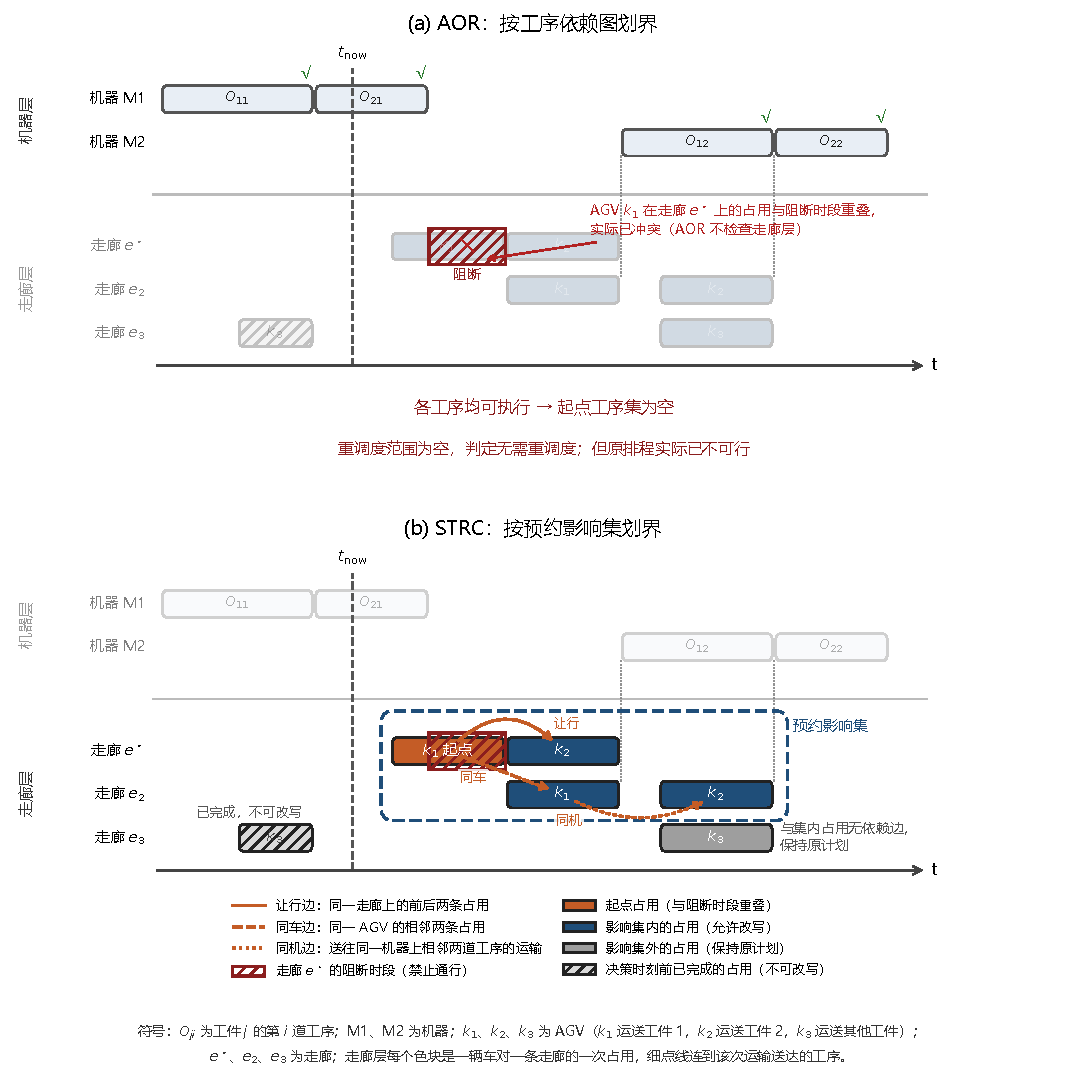
\includegraphics[width=0.72\linewidth]{figures/fig_strc_motivate_CN}
\caption{动机示意：同一份排程、同一次走廊阻断，两种划界方法检查的层不同。
每幅上层为机器层（工序甘特），下层为走廊层（预约表），斜纹框为走廊 \(e^{\star}\) 上的阻断时段，竖虚线为决策时刻 \(t_{\mathrm{now}}\)。
(a)~AOR 只检查机器层：各工序均可执行，起点工序集为空，判定无需重调度；但走廊层上 AGV \(k_1\) 的占用已与阻断冲突，原排程实际不可行。
(b)~本文方法检查走廊层：与阻断重叠的 \(k_1\) 占用成为起点；\(k_2\) 在 \(e^\star\) 上紧随其后，经让行边纳入；
\(k_1\) 在 \(e_2\) 上的下一条占用经同车边纳入；\(k_1\)、\(k_2\) 在 \(e_2\) 上分别送往同一台机器 M2 上相邻的 \(O_{12}\)、\(O_{22}\)，二者以同机边相连。
这四条占用构成预约影响集（虚线框）；\(k_3\) 的占用与集内占用之间没有依赖边，保持原计划；\(t_{\mathrm{now}}\) 前已完成的占用不可改写。}
\Description{上下两幅，画的是同一份排程。每幅上层是两台机器上的四道工序，下层是三条走廊上的 AGV 占用，
走廊 e-star 上有一段阻断时段，一条竖虚线标出决策时刻。上幅中机器层正常显示、每道工序打勾，走廊层淡化，
AGV k1 在 e-star 上的占用与阻断重叠处画红叉，底部写明起点工序集为空、判定无需重调度、但原排程已不可行。
下幅中机器层淡化、走廊层正常显示：k1 在 e-star 上的占用标为起点，箭头沿让行边指向 k2 在 e-star 上的占用，
沿同车边指向 k1 在 e2 上的占用，再沿同机边指向 k2 在 e2 上的占用；这四条占用被虚线框圈为预约影响集，
e3 上 AGV k3 的一条占用在框外，标为与集内占用无依赖边、保持原计划，另一条在决策时刻前已完成。}
\label{fig:motivate}
\end{figure}

\subsection{主要思想与贡献}
\label{sec:contributions}

本文的主要思想有两点。
其一，在用预约表保证 AGV 无冲突通行的柔性作业车间中，扰动后的重调度范围应划定在走廊占用上，
而不是只划定在工序上：走廊阻断这类扰动只使占用失效，失效再沿让行关系在 AGV 之间传播，
这些都只能在由走廊占用及其依赖关系构成的预约依赖图上表达。
其二，执行期扰动要求立即给出可继续执行的排程，因此在划定的范围内只做局部恢复，
不重新启动种群搜索，使响应保持在毫秒量级。

据此，本文把扰动后的恢复分为两步：先划定重调度范围，再只在范围内修复。
重调度范围从与扰动冲突的占用出发，沿占用之间的依赖关系，逐步纳入可能因此须改写的占用；
范围以外的占用在修复中原样保留。
该范围只由原排程中的依赖关系确定，不取决于随后采用哪种修复算法，因此同一扰动下得到的范围唯一、可以复现。

本文的贡献如下，后文分别记为 C1、C2、C3。
\begin{enumerate}[label=\textbf{C\arabic*.},leftmargin=2.2em,itemsep=0.4em]
\item \textbf{指出工序依赖图无法刻画的一类失效。}
B 类扰动下，按受影响工序划定的范围为空，而原排程已不可行，延误还会沿让行关系传给后续 AGV；
在全部 \(\NPairs\) 对走廊阻断实验中均如此（第~\ref{sec:e1}~节）。

\item \textbf{提出时空预约闭包（\STRC），以预约影响集作为重调度范围。}
以与受扰时段重叠的走廊占用为起点，沿让行、同一 AGV、同一工件与同一机器上的接续关系取传递闭包，
所得集合即预约影响集。在四类扰动下影响集均非空，且在 A 类扰动下包含按工序依赖图划定的范围，不会漏掉原方法已纳入的占用（第~\ref{sec:e6}~节）。

\item \textbf{给出与该划界匹配的毫秒级局部恢复。}
影响集外保持原计划，集内与扰动直接冲突的运输在全图上重规划、其余运输先沿原路线只改时刻；仍不可行时再按既定顺序放宽。
在同一回放程序下只替换划界对象，走廊阻断下得到可继续执行排程的对数由 \(\FeasRone\) 升至 \(\FeasRtwo\)（第~\ref{sec:e3}~节）；
按工序依赖图划界失败，是因为它判定无需重调度、未改动任何占用，而不是改路能力不足。整个恢复耗时为毫秒量级，比热启动全局重调度低两到三个数量级（第~\ref{sec:e5}~节）。
与改写全部尚未完成运输的对照相比，划界本身的收益在于冻结集不被其他运输的重规划挤动：
在规模批次上被改动的占用明显减少，而耗时相当（第~\ref{sec:boundary}~节）。
\end{enumerate}

\subsection{篇章结构}

第~\ref{sec:related_work}~章按四类回顾相关工作：作业车间如何按工序或时间轴划定重调度范围、
铁路调度如何表达排他资源上的占用先后、无冲突多车路径如何做局部重规划，
以及考虑运输的柔性作业车间把边界划在何处，并据此说明本文与已有工作的区别。
第~\ref{sec:problem}~章给出走廊预约设定与执行期恢复问题：
车间、走廊预约表与工序依赖图，两类扰动，以及恢复须满足的条件。
第~\ref{sec:strc}~章给出恢复方法：先以时空预约闭包求出预约影响集作为允许改写的范围，
说明其依赖边与对外封闭等性质；B 类扰动下，集外占用原样预提交，集内按重规划与只改时刻两层做分层回放，
仍不可行时先放宽搜索，再逐级扩大允许改写的范围；A 类扰动下改用换车与改派。
第~\ref{sec:experiments}~章说明对照方法，报告可行性、算法耗时、占用改动比例与完工时间，
并用案例甘特图在工序时间轴上展示统计结果对应的改动形态。
第~\ref{sec:conclusion}~章总结全文的主要结论，并讨论局限与未来工作。

%% =====================================================================
\section{相关工作}
\label{sec:related_work}
%% =====================================================================

%% 相关工作按问题类型回顾,不作「四层定位」。旧文献以引文簇保留,叙述以近作为主。

动态调度的一个基本问题是划定重调度范围：扰动发生后，哪些工序、走廊占用或 AGV 的原有安排须重新规划，
范围以外的安排则保持原计划不变。
对于重调度范围应划在哪类对象上，已有文献给出了不同做法：工序或时间轴、排他资源上的占用先后、
多智能体路径规划中受影响的智能体，以及带运输的柔性作业车间中的工序集合。
下面按这四类回顾各自做了什么、尚未覆盖什么，并在表~\ref{tab:position} 中把它们与本文在问题设定和重调度范围上逐项对比。

\subsection{作业车间的局部重调度}
\label{sec:rw_aor}

对机器故障、插单等工序事件，按受影响工序划定重调度范围，在带 AGV 的动态调度中仍被采用。
Zhang 等~\cite{zhang2023energy} 处理机器故障与插单，恢复范围取故障后尚未加工的工序；
Tang 等~\cite{tang2026dynamic} 按扰动影响把工序与配送任务分为保留、继续、重构，
并把完全重调度、部分重调度与右移并列，指出右移保住稳定性、让出优化空间。
这一做法的代表是受影响工序重调度（AOR）及其改进 MAOR~\cite{subramaniam2003maor}：
只重排被扰动直接或间接波及的工序。
沿时间轴划界与失败后逐步扩大重调度范围同样已有文献研究过。match-up 方法从扰动时刻向后寻找能够回到原排程的时间点，只重排这段时间内的工序：
Qiao 等~\cite{qiao2012single} 将其用于半导体制造系统，并与右移重调度作了比较；
Salido 等~\cite{salido2017rescheduling} 在机器可变速的作业车间中先用 match-up 确定重调度区间，再在区间内降低能耗。
增量扩大时间窗的 Local Rescheduling~\cite{kuster2007local} 则在修复失败后逐步放宽范围。
右移则不判定谁受影响，把未完成部分整体后推。
滚动时域方法把长时域问题拆成相互重叠的短时域子问题依次求解~\cite{li2025learning}，
分解方法则按优先约束结构把工件集拆成依次排序的子块~\cite{margot2003decompositions}；
综述见~\cite{vieira2003rescheduling,ouelhadj2009survey}。

可见，先划定范围、再在范围内局部重调度是通行做法，但上述工作都以受扰工序为划界起点；
扰动只作用于走廊时，就没有这样的起点（第~\ref{sec:introduction}~章）。

\subsection{排他资源上的占用先后}
\label{sec:rw_ag}

「谁先占用同一排他资源」被建成图，在铁路调度中已有系统研究。
Mascis 与 Pacciarelli~\cite{mascis2002alternative} 的 alternative graph
把析取图推广为：顶点是作业对闭塞区段的占用，固定弧表示路径先后，
成对的 alternative arc 表示谁先通过该区段。
D'Ariano 等人~\cite{dariano2007branch} 用该模型做列车实时重调度，
扰动后重算无冲突时刻表，并尽量接近原计划。
alternative arc 刻画的是两列车通过同一闭塞区段的先后次序；
本文中两辆 AGV 通过同一走廊时的让行关系，也是同一排他资源上的这种占用先后。

在 alternative graph 中，每一处争用对应一对互斥的弧（甲先通过，或乙先通过），
排程即从每对中选定一条，使图中不出现正权回路、时刻表可行，并尽量使目标最优；
占用先后因此是待优化的决策变量。
铁路模型把闭塞区段当作机器，列车的运行与区段占用在同一张图上，
区段不可用即直接表现为图上的事件，因此不存在「范围划在工序依赖图上而遗漏走廊阻断」的问题。
本文则在计划已排定、先后已确定之后使用这类关系：不再选择先后，
只沿既定的让行与接续关系判断扰动后哪些走廊占用须重新规划。

\subsection{无冲突多车路径的局部重规划}
\label{sec:rw_mapf}

在多智能体路径规划中，只为受影响者进行重调度、其余视为动态障碍，已是标准做法。
Švancara 等人~\cite{svancara2019online} 在在线 MAPF 中给出
% selfcheck:allow-term 「受影响集合」此处指 MAPF 独立性检测的输出,不是本文机制的名字
Replan All、Replan Single 与 Replan Affected，并用在线独立性检测确定受影响集合；
Malka 等人~\cite{malka2024online} 在地图不准确时，同样只为受观测变化影响的智能体重规划。
% selfcheck:allow-term 「时空占用」是 MAPF 的既有术语,此处在转述该文献,不指本文的走廊占用
无冲突路径规划把时空占用作为一等约束，但起终点通常由外部给定~\cite{zhang2024guidance}。

这类工作只有智能体的起终点，没有工件—工序—机器指派，
因而不会出现「重调度范围按工序依赖图划定、走廊阻断因找不到受影响工序而被遗漏」的情形。
% selfcheck:allow-term 「受影响集合」此处是两法共用的中性说法,后半句即在说它是检测算法的输出
就受影响集合如何得到而言，MAPF 用独立性检测找出受影响的智能体，得到的是检测算法的输出，随实现方式和停止条件而变。
本文给出的预约影响集则不同：依赖边一经给定，一条占用是否属于该集，
只取决于它能否从起点沿这些边到达，与随后用哪一种路径规划算法无关
（第~\ref{sec:containment}~节）。

\subsection{考虑运输的柔性作业车间调度}
\label{sec:rw_position}

考虑 AGV 运输的柔性作业车间调度已有系统综述~\cite{xin2025review}。
近期组合优化工作仍普遍把运输时间设为按起止位置读取的常数矩阵，
并在此之上发展约束规划与知识引导搜索~\cite{meng2025cp,qin2026knowledge}；
也有工作让运输时间随载重变化，并以聚合的拥堵延误项近似 AGV 之间的相互影响~\cite{jafarian2026integrated}。
这两种约定都不记录 AGV 对具体路段的占用，走廊阻断在模型里没有对应对象，无法被检验。

一旦用预约表记录走廊占用时段，加工先后与走廊占用同时进入模型。
拥堵感知派车可用局部密度等代理量选车，而不改机器指派~\cite{kim2026congestion}。
把柔性指派与无冲突运输联合建模的工作相对较少：
van Os 与 Basten~\cite{vanos2026exact} 形式化了带无冲突运输约束的柔性作业车间调度，
并以分解方法在多数基准算例上取得可证最优，少数因限时未能保证最优性；
两阶段方案先固定排产再消解 AGV 冲突~\cite{sun2023integrated}；
亦有学习层排产、路径层消冲突、并以有限反馈连接的框架~\cite{li2026framework}。
但这些工作回答的是开工前如何排出可行且质量好的无冲突排程，并不处理执行期扰动，
例如 Sun 等~\cite{sun2023integrated} 假定 AGV 始终可用、不发生故障。
反过来，第~\ref{sec:rw_aor}~节中处理执行期扰动的带 AGV 动态调度工作又不建模 AGV 之间的走廊争用，
例如 Zhang 等~\cite{zhang2023energy} 忽略 AGV 之间的碰撞。
也就是说，在考虑运输的柔性作业车间调度研究中，走廊预约表与执行期扰动尚未同时出现；
本文研究的正是二者同时出现的情形（第~\ref{sec:e1}~节实测 \PassMiss）。

\subsection{本文定位}
\label{sec:rw_claim}

\begin{table*}[t]
\centering
\caption{相关工作与本文在问题设定和重调度范围上的对比。
\cmark\ 表示具备，\xmark\ 表示不具备，— 表示不适用（该类工作不划定局部重调度范围）。
「占用时段」指模型显式记录各 AGV、智能体或列车占用路段（闭塞区段、时空格点）的时段。
「划定在」为范围内允许改写的对象，本文中，工序、AGV 与走廊上的扰动均先转换为起点占用，再沿依赖边划定范围；
「失效沿哪些途径纳入」以失效所经的共享资源表示划界时追踪的传播途径；
「考虑走廊扰动带来的失效」指走廊阻断等只作用于走廊的扰动发生时，失效的占用全部落入重调度范围。}
\label{tab:position}
\small
\setlength{\tabcolsep}{3pt}
\begin{tabular}{@{}p{0.23\linewidth}ccp{0.14\linewidth}p{0.15\linewidth}p{0.17\linewidth}c@{}}
\toprule
& \multicolumn{3}{c}{\textbf{问题设定}} & \multicolumn{3}{c}{\textbf{重调度范围}} \\
\cmidrule(lr){2-4}\cmidrule(l){5-7}
\textbf{代表工作} &
\makecell{\textbf{工序与}\\\textbf{机器指派}} &
\makecell{\textbf{占用}\\\textbf{时段}} &
\textbf{执行期扰动} &
\textbf{划定在} &
\textbf{失效沿哪些途径纳入} &
\makecell{\textbf{考虑走廊扰动}\\\textbf{带来的失效}} \\
\midrule
AOR~\cite{subramaniam2003maor} &
\cmark & \xmark & 工序事件 & 受影响工序 & 工件、机器 & \xmark \\
match-up~\cite{qiao2012single,salido2017rescheduling}、LRS~\cite{kuster2007local} &
\cmark & \xmark & 工序事件 & 时间窗 & 时间窗逐步放宽 & \xmark \\
带 AGV 的动态调度~\cite{zhang2023energy,tang2026dynamic} &
\cmark & \xmark & 设备故障、插单 & 工序与运输 & 按扰动类型分类 & \xmark \\
铁路实时重调度~\cite{mascis2002alternative,dariano2007branch} &
\xmark & \cmark & 列车延误 & 全部列车 & —（整体重排） & \cmark \\
在线 MAPF~\cite{svancara2019online,malka2024online} &
\xmark & \cmark & 新任务、地图变化 & 受影响智能体 & 智能体间路径冲突 & \cmark \\
常数或聚合运输时间~\cite{meng2025cp,qin2026knowledge,jafarian2026integrated} &
\cmark & \xmark & 无（开工前） & — & — & — \\
一体化无冲突排程~\cite{vanos2026exact,sun2023integrated,li2026framework} &
\cmark & \cmark & 无（开工前） & — & — & — \\
\midrule
\textbf{本文} &
\cmark & \cmark & \textbf{工序事件、AGV 故障与走廊扰动} & \textbf{走廊占用} & \textbf{走廊、AGV、工件、机器} & \cmark \\
\bottomrule
\end{tabular}
\end{table*}

如表~\ref{tab:position} 所示，所列工作中没有一类同时具备工序与机器指派、占用时段与执行期扰动三项设定：
铁路调度与在线 MAPF 记录占用时段、处理执行期扰动，但没有工序与机器指派；
有工序与机器指派、处理执行期扰动的工作又不记录占用时段。
本文在三项设定兼备时，把重调度范围改到走廊占用及其让行、接续关系上，得到由这些关系唯一确定的预约影响集。

表中最后两列体现了本文划定范围的两条原则。
其一，范围须纳入全部失效的占用，否则修复后的排程仍不可行；
在此前提下，沿传播途径不可达的占用不纳入，在修复中原样保留。
其二，传播途径须与失效实际传播的渠道一致：缺少一类途径，经该类资源受波及的占用就不会被纳入，
AOR 只沿工件与机器两类途径扩展，走廊阻断下因此得到空范围；纳入并不传播失效的关系，则只会无谓扩大范围。
本文的四类途径——走廊（让行）、AGV、工件、机器——对应模型中约束走廊占用时刻的四类共享资源。

%% =====================================================================
\section{走廊预约设定与执行期恢复问题}
\label{sec:problem}
%% =====================================================================

\subsection{系统设定与记号}
\label{sec:system_brief}

本文研究的问题属于带无冲突运输约束的柔性作业车间调度，
因此以 van Os 与 Basten~\cite{vanos2026exact} 对该问题的形式化为基础建立模型，二者在预约对象上的差异见第~\ref{sec:reservation}~节。
本节给出后文各章共用的对象与记号。
扰动前的可行排程 \(\mathcal{S}^0\) 视为给定输入：
后文的划界只依赖 \(\mathcal{S}^0\) 本身（机器指派、加工顺序与预约表），
不依赖它在 \(t=0\) 由何种算法求得，因此 \(\mathcal{S}^0\) 可以来自任意排程方法。

\subsubsection{车间与排程}
\label{sec:shop}

车间路网 \(G=(V,E)\) 强连通，\(v_{\mathrm{in}},v_{\mathrm{out}}\in V\) 分别为毛坯库与成品库，
二者分设于物流的两端。车间有 \(n\) 个工件与机器集合 \(M\)，
每台机器 \(m\) 位于固定节点 \(\mathrm{loc}(m)\)；
\(N_A\) 辆 AGV 同构，每次只运一个工件，记 \(K=\{1,\ldots,N_A\}\)。
工件 \(j\) 有固定工序链 \(O_{j1}\to\cdots\to O_{jn_j}\)；
工序 \(O_{ji}\) 的候选机器集为 \(\Omega_{ji}\subseteq M\)，在机器 \(m\) 上耗时
\(t^P_{jim}\)。一份完整排程须同时确定以下四项：
(i)~机器指派 \(x\)：为每道工序选择一台机器；
(ii)~加工顺序 \(\pi\)：确定每台机器上各工序的加工先后；
(iii)~AGV 指派 \(y\)：为每次搬运选定 AGV；
(iv)~路径规划：为每次 AGV 行驶规划 \(G\) 上的无冲突路径及各段的通行时刻。
记
\[
\mathcal{S}=(x,\,\pi,\,y,\,R),
\]
其中预约表 \(R\) 是第 (iv) 项的显式记录，定义见下。

运输任务不是事先给定的固定参数，而是由机器指派 \(x\) 决定：
工件从毛坯库 \(v_{\mathrm{in}}\) 出发，同一工件相邻两道工序被指派到位于不同节点的机器上时需要一次搬运，
完成末道工序后还须送入成品库 \(v_{\mathrm{out}}\)；
指派一旦改变，搬运的次数与起讫节点也随之改变。
为工序 \(O_{ji}\) 送料的一次搬运称为\emph{运输} \((j,i)\)（送入成品库的那次记为 \((j,n_j+1)\)），
由一辆 AGV 一次完成，依次包括：从当前位置空载驶往取件节点（\emph{空驶}）、在取件节点等工件完成前一道工序、
载着工件驶往目的节点（\emph{载运}），以及送达后的停放或离场（见第~\ref{sec:reservation}~节）。
装卸时间取为零：载运在「空驶抵达取件节点」与「工件完成前一道工序」二者中较晚的时刻出发，
送达时刻即后一道工序可以开工的时刻。
后文判定哪些占用允许改写、哪些保持原计划，以及改路，都以单次运输为基本单位，
而不是以整道工序或整个工件为单位；每条占用都标有它所属的运输 \(u\)，
记 \(\tau(X)\) 为占用集合 \(X\) 所属运输的集合。

\subsubsection{走廊与节点预约}
\label{sec:reservation}

每条走廊 \(e\in E\) 是排他资源，通行时间 \(\tau_e\) 已知。走廊按单车道处理：
AGV 无论朝哪个方向通行，都占用整条走廊，因而任一时刻至多一辆 AGV 在 \(e\) 上，
迎面相遇与同向超车都不会发生。
这对应 AGV 车间中常见的单车道窄通道与分区占用控制；
双车道走廊可在路网中表示为两条走廊。
走廊占用取半开区间：后一辆 AGV 可以恰好在前一辆 AGV 驶离的时刻进入。

路网节点分为三类：库区（毛坯库 \(v_{\mathrm{in}}\) 与成品库 \(v_{\mathrm{out}}\)）、机器所在节点（下称\emph{机器节点}）与路口（走廊交汇处），
容量 \(\kappa(v)\) 按类型给定：库区不限；机器节点由一个交接位与若干待命位组成，容 \(c\) 辆；路口容 \(1\) 辆。
每个机器节点只经一条支线与路网相连，AGV 仅在以该机器为起点或终点时才驶入，不会途经它前往其他节点。
AGV 只在节点上等待，不在走廊中途停车；在节点上的等待计入停留。
AGV 驶离节点后，车身完全让出该节点还需一段时间，为此令节点的占用延续到离开后 \(h\) 个时间单位（净空时距）。
送达后，若目的节点此后一直有空位，AGV 就停放于此（停放不设终点，直到它下一次出发）；否则驶往最近的库区，下称\emph{离场}。
若一次运输要在某机器节点交接，而该节点已停满空闲 AGV，则最早停下的空闲 AGV 先驶往最近的库区腾位，下称\emph{驱离}；
离场与驱离的行程都记在引起它的那次运输名下。
本文实验取 \(c=3\)（一个交接位与两个待命位）、\(h=0.5\)。

预约表 \(R\) 记录两类占用。一条\emph{走廊占用}为
\[
r=(e,\,[t^s,t^e),\,k,\,u),
\]
即 AGV \(k\) 在 \([t^s,t^e)\) 占用走廊 \(e\)，所属运输为 \(u\)；
一条\emph{节点停留}为 \(\sigma=(v,\,[\alpha,\beta+h),\,k,\,u)\)，其中 \(\alpha\)、\(\beta\) 为到达与离开时刻，
停放尚未结束时 \(\beta=\infty\)。
同一走廊上任意两条不同占用的区间互不相交；任一时刻，节点 \(v\) 上的停留数不超过 \(\kappa(v)\)。
规划路径时只使用预约表中尚空的时段与车位，
因此新写入的占用不会违反上述约束，无需事后再做冲突检测。

路径规划模块是改路与各对照方法共用的基础模块：给定 AGV、起点、取件节点、工件就绪时刻、目的节点与当前预约表 \(R\)，
它为这次运输一次性规划完整轨迹（空驶、等件、载运，以及送达后的停放或离场，必要时含驱离），并把各条占用写回 \(R\)。
节点有了容量，AGV 便不能在任意节点上任意久地等待，节点上的空位随时间时有时无；
本文因此采用安全区间规划（SIPP）~\cite{phillips2011sipp,kasaura2022sipp}：
搜索标签为（节点，该节点上的安全区间，是否已取件，到达时刻），安全区间即节点上除本车外停留数低于容量的极大连续时段，
每个（节点，安全区间，阶段）只保留最早到达的标签。
本文不改动这一模块，只改变\emph{哪些}运输交给它重新规划，以及允许它使用哪些走廊（第~\ref{sec:strc}~章）。
有界修复对它只要求一点：能在已有预约之上为单辆 AGV 规划轨迹，并把其占用写回 \(R\)；
时空 A*~\cite{silver2005cooperative} 等逐车规划方法同样满足这一要求。

\subsubsection{工序依赖图与预约依赖图}
\label{sec:two_graphs}

% selfcheck:allow-term 「任务图」是 B13 裁定保留的同义登记,兼作 \(G_T\) 下标的来由
工序依赖图 \(G_T=(T_T,E_T)\)（文献中亦称任务图，下标 \(T\) 取自 task）以工序为顶点，
有向边表示两道工序之间的先后约束，分两类：
\emph{工件先后}，即同一工件的工序 \(O_{ji}\) 指向它的下一道工序 \(O_{j,i+1}\)；
\emph{同机先后}，即同一台机器上的工序指向在该机器上紧随其后加工的工序。
预约依赖图 \(G_R\) 以预约表中的占用（走廊占用为主，另含受阻走廊两端的节点停留）为顶点，有向边 \(r\to r'\) 表示 \(r\) 一旦改写、
\(r'\) 也可能须随之改写。其中一道工序 \(O_{ji}\) 的\emph{运输占用}，指运输 \((j,i)\) 产生的占用。
边分四类，对应占用之间四种「一个推迟、另一个跟着受影响」的关系：
\begin{itemize}[leftmargin=1.5em,itemsep=0.1em]
\item \textbf{让行：}同一条走廊上，两辆不同的 AGV 先后通过。前车推迟，后车须等前车驶离，也只能推迟。
\item \textbf{同车：}同一辆 AGV 先后走过的两段走廊。车在前一段推迟，到达下一段的时刻也随之推迟。
\item \textbf{同工件：}同一工件相邻两道工序的运输。前一道工序的物料晚到，加工晚完成，下一道工序的运输就只能晚出发。
\item \textbf{同机：}同一台机器上先后加工的两道工序的运输。前一道工序晚开工，机器晚空出，后一道工序只能推后开工，为它送料的运输也可能须随之调整。
\end{itemize}
前两类来自走廊与 AGV 这两种通行资源，后两类由工序依赖图中的工件先后与同机先后对应而来；精确的连边条件见定义~\ref{def:dep}。
两张图的顶点集不相交：一边是加工，一边是通行。走廊阻断这类扰动因此在 \(G_T\) 上找不到起点工序，
而在 \(G_R\) 上，与受扰时段重叠的占用就是起点（命题~\ref{prop:miss}）。
图~\ref{fig:graphs} 对照这两张图，表~\ref{tab:notation} 汇总本节及后文用到的记号。

\begin{figure}[tbp]
\centering
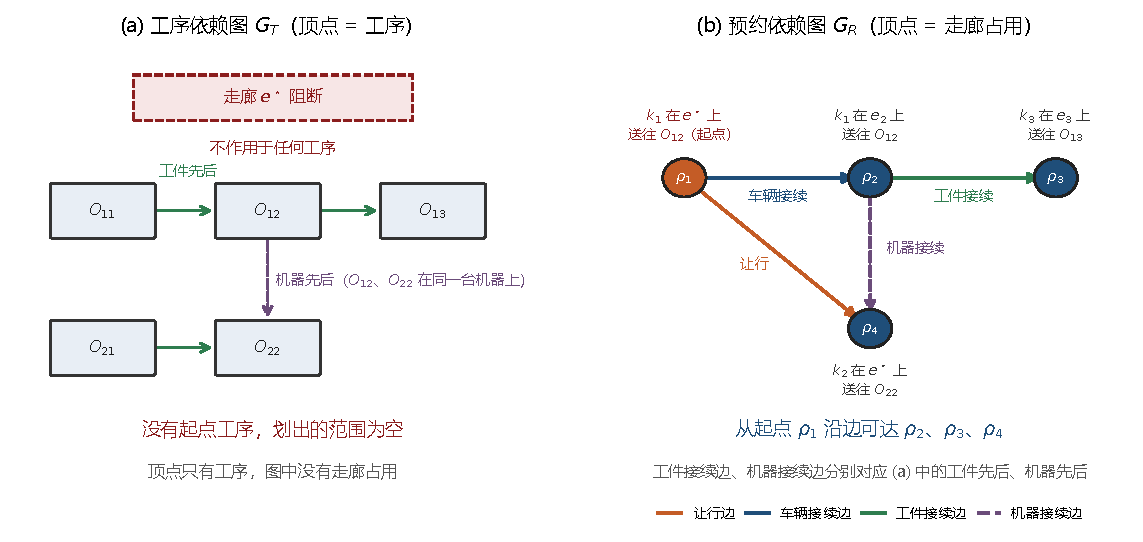
\includegraphics[width=\linewidth]{figures/fig_strc_graphs_CN}
\caption{两张图的顶点集不相交（构造示意）。
(a)~工序依赖图 \(G_T\)，顶点是工序，走廊 \(e^\star\) 阻断不作用于任何工序，找不到起点工序；
(b)~预约依赖图 \(G_R\)，顶点是同一排程中的走廊占用，每个顶点旁注明承运 AGV、所在走廊与所送工序。
与阻断时段重叠的 \(\rho_1\) 为起点，沿四类依赖边（定义~\ref{def:dep}）可达其余占用：
\(\rho_1\to\rho_2\) 为同一 AGV 的相邻占用，\(\rho_1\to\rho_4\) 为同一走廊上的先后占用；
\(\rho_2\to\rho_3\) 与 \(\rho_2\to\rho_4\) 分别由 (a) 中 \(O_{12}\to O_{13}\) 的同工件先后与 \(O_{12}\to O_{22}\) 的同机先后得到。}
\Description{并排两幅。左幅是工序依赖图，五个工序方框之间有同工件先后与同机先后的箭头，
顶部一条虚线框标出走廊阻断，注明不作用于任何工序，下方写着没有起点工序、划出的范围为空。
右幅是预约依赖图，四个圆形顶点表示走廊占用，旁边注明承运 AGV、所在走廊与所送工序；
起点 rho1 经同车边指向 rho2、经让行边指向 rho4，rho2 经同工件边指向 rho3、经同机边指向 rho4。}
\label{fig:graphs}
\end{figure}

\begin{table}[t]
\centering
\caption{本文常用记号}
\label{tab:notation}
\small
\begin{tabular}{@{}ll@{}}
\toprule
\textbf{符号} & \textbf{含义} \\
\midrule
\(G=(V,E)\), \(\tau_e\) & 走廊路网；走廊 \(e\) 的通行时间 \\
\(v_{\mathrm{in}},v_{\mathrm{out}}\), \(\mathrm{loc}(m)\) & 毛坯库、成品库；机器 \(m\) 的机器节点 \\
\(\kappa(v)\), \(c\), \(h\) & 节点容量（库区 \(\infty\)、机器节点 \(c\)、路口 \(1\)）；机器节点容量；净空时距 \\
\(x,\pi,y\) & 机器指派、加工顺序、AGV 指派 \\
\(R\), \(r=(e,[t^s,t^e),k,u)\) & 预约表；一条半开走廊占用（AGV \(k\)，所属运输 \(u\)）\\
\(\sigma=(v,[\alpha,\beta+h),k,u)\) & 一条节点停留 \\
\(\tau(X)\) & 占用集合 \(X\) 所属运输的集合 \\
\(G_T\) / \(G_R\) & 工序依赖图 / 预约依赖图 \\
\(\mathcal{S}^0,\mathcal{S}'\) & 扰动前排程、恢复后排程 \\
\(\mathcal{D},\,t_{\mathrm{now}}\) & 扰动事件、发生（决策）时刻 \\
\(T_{\mathrm{direct}},\,T_{\mathrm{impact}}\) & 工序依赖图上直接受扰的工序 / \(\theta\)-步纳入范围 \\
\(\mathrm{Src}(\mathcal{D})\), \(U\) & 作为起点的占用（走廊部分 \(\mathrm{Src}_E\)、节点部分 \(\mathrm{Src}_V\)）；允许改写的占用集合 \\
\(\mathrm{Cl}(\cdot)\) & 预约影响集（由 \STRC 得到）\\
\(W,\ Q_0,\ T,\ F\) & 改写集 \(\tau(\mathrm{Cl})\)、重规划集、平移集 \(W\setminus Q_0\)、冻结集 \\
\(\varphi\) & 受扰未来工序比例（规模扫描）\\
\bottomrule
\end{tabular}
\end{table}

\subsection{执行期假设}
\label{sec:assumptions}

执行期约定与物理设定如下。其中 A1--A4 由全部对照方法共用，以便把结果归因到重调度范围
如何划定，而不是模型差异；A5 只约束本文方法，作为对照的全局重调度还可以改变机器指派与加工顺序：

\begin{enumerate}[label=\textbf{A\arabic*.},leftmargin=*,topsep=2pt,itemsep=2pt]
\item \textbf{初始排程可行。} \(\mathcal{S}^0\) 在扰动前通过无冲突校验；预约表与工序时间表一致。
\item \textbf{已开始的行程不回溯。} 只改写 \(t^s\ge t_{\mathrm{now}}\) 的尚未开始的走廊占用、
尚未结束的节点停留中 \(t_{\mathrm{now}}\) 之后的部分，以及未完工工序；其余占用字段不可改写。
在 \(t_{\mathrm{now}}\) 时已驶入某条走廊的 AGV 走完这条走廊：车不能在单车道中途折返，也不能退回已让给后车的路口。
由此，走廊阻断只拦截此后的进入，其\emph{生效时段}从 \(\max\{t_a,\,t_{\mathrm{now}},\,\text{该走廊上进行中占用的结束时刻}\}\) 开始；
通行变慢只拉长此后进入的通行，已开始的那一段保持原时长；
AGV 故障时，故障车走完当前这条走廊，在到达的节点上退出路网，此后不再占用任何走廊与车位。
\item \textbf{单次、完全观测。} 扰动在 \(t_{\mathrm{now}}\) 被完整观测，且不与其它扰动叠加。
本文不研究以下情形：多个扰动相继到达；扰动的信息（如阻断持续时间）在发生时只能估计且可能有误；
随新信息到达而反复重调度。
\item \textbf{走廊排他、节点限容、AGV 同构。} 走廊仍为排他半开资源，节点容量与净空时距如第~\ref{sec:reservation}~节；
阻断以附加占用的形式写入预约表，即在该走廊上写入一段不准通行的时段，下称\emph{阻断时段}。
充电、加减速与装卸时长不建模；全部 AGV 在计划开始时空载停于毛坯库 \(v_{\mathrm{in}}\)。
\item \textbf{允许的恢复动作。} B 类扰动保持原机器指派 \(x\) 与加工顺序 \(\pi\)，只改路；
失败时扩大允许改写的占用集合。A 类故障额外允许：AGV 故障时停用故障 AGV，由其他 AGV 接替其任务；
机器故障时把该机器上未完工的工序改派到其它可行机器。加工顺序 \(\pi\) 始终不变，不重开搜索。
实验中的全局重调度对照可以改 \(x\) 与 \(\pi\)（第~\ref{sec:vs_r0}~节）。
\end{enumerate}

\subsection{两类扰动}
\label{sec:disturbance_classes}

\begin{definition}[A/B 类扰动]
\label{def:ab}
若扰动直接使某些工序的指派或\emph{可执行性}失效（机器故障、显著工时偏差、插单、
AGV 故障等），称其为 \textbf{A 类}；若扰动只使某些走廊在某段时间内不可用、而不使任何工序
不可执行（走廊阻断、走廊通行变慢等），称其为 \textbf{B 类}。
\end{definition}

\begin{remark}[AGV 故障为何属于 A 类]
\label{rem:agv_class}
AGV 故障不改动任何工序的机器指派，乍看应与走廊阻断同类。但定义~\ref{def:ab} 的判据是
\emph{可执行性}而非指派：AGV 发生故障后，它承运的工序在原计划下无法开工。
只要方法记录了每辆 AGV 承运哪些工序，这些工序就可以作为工序依赖图上的起点，
按工序划界得到的范围不为空，因此 AGV 故障归 A 类。
若方法只记录工序与机器（AOR 的常见实现即如此），AGV 故障同样会得到空范围。
第~\ref{sec:e6}~节实现的 AOR 记录了各 AGV 承运的工序，因此在 AGV 故障下给出非空范围。
\end{remark}

\begin{definition}[工序依赖图上的直接集与影响域]
\label{def:task_impact}
对扰动 \(\mathcal{D}\)，令 \(T_{\mathrm{direct}}(\mathcal{D})\) 为因机器故障、AGV 故障或工序失效
而无法按原计划执行的工序集合。对 B 类走廊扰动约定 \(T_{\mathrm{direct}}=\varnothing\)。
在 \(G_T\) 上从 \(T_{\mathrm{direct}}\) 出发，沿工件先后边与同机先后边最多走 \(\theta\) 步，
所能到达的工序（含 \(T_{\mathrm{direct}}\) 本身）记为 \(T_{\mathrm{impact}}(\mathcal{D},\theta)\)。
实验中的对照实现只沿工件先后边扩张（第~\ref{sec:vs_r0}~节）。
\end{definition}

\begin{definition}[作为起点的占用]
\label{def:seeds}
起点集 \(\mathrm{Src}(\mathcal{D})=\mathrm{Src}_E\cup\mathrm{Src}_V\) 按扰动类型给出，
\(\mathrm{Src}_E\) 为其中的走廊占用，\(\mathrm{Src}_V\) 为其中的节点停留（只有走廊阻断取节点停留，其余类型 \(\mathrm{Src}_V=\varnothing\)）。
各类型都只取 \(r.t^e>t_{\mathrm{now}}\) 的占用，即在决策时刻尚未结束的占用；已经结束的占用不作为起点。
\begin{enumerate}[label=(\alph*),leftmargin=1.6em,itemsep=0.15em]
\item \textbf{走廊阻断} \(\mathcal{D}=(e,[t_a,t_b))\)：记 \([t_a',t_b)\) 为其生效时段（假设 A2：已开始的行程不回溯）。
起点分两部分：走廊部分
\(\mathrm{Src}_E=\{\,r:\ r.e=e,\ [r.t^s,r.t^e)\cap[t_a',t_b)\neq\varnothing\,\}\)，即走廊 \(e\) 上与生效时段重叠的占用；
节点部分 \(\mathrm{Src}_V\) 为 \(e\) 两端节点上与生效时段重叠的停留。
阻断使车在走廊口等待，首先受牵连的是在这两个节点上停留、或随后要进入这两个节点的车，故把这些停留也作为起点。
有多处短暂阻断时，取各阻断各自起点的并集。
\item \textbf{通行变慢} \(\mathcal{D}=(e,[t_a,t_b),\rho)\)：
\(\mathrm{Src}=\{\,r:\ r.e=e,\ r.t^s\ge t_{\mathrm{now}},\ [r.t^s,r.t^e)\cap[t_a,t_b)\neq\varnothing\,\}\)，
即走廊 \(e\) 上尚未开始、且与受扰时段重叠的占用。原排程按未变慢的通行时间写出，这些占用无法按原时刻完成。
与阻断不同，受扰时段内该走廊仍可通行，只是落在受扰时段内的那部分通行时间按倍率 \(\rho\) 加长。
\item \textbf{AGV 故障} \(\mathcal{D}=(k)\)：该车尚未结束的全部占用
\(\{\,r:\ r.k=k\,\}\)。
\item \textbf{机器故障} \(\mathcal{D}=(m,F)\),\(F\) 为该机器上尚未完工的工序：
对每个工件取 \(F\) 中最小工序号 \(i_{\min}(j)\)，起点占用为各工件自该工序起（含）的全部
尚未结束占用。之所以沿工件链向后取，而不只取该工序自身的占用，是因为该工序的进站运输可能已在
\(t_{\mathrm{now}}\) 前结束：若只取自身，起点占用会变空或偏少，预约影响集覆盖的工序反而少于
工序依赖图上的影响域，两种划界的比较就不公平——差别来自起点取法，而不是划界对象。
\end{enumerate}
\end{definition}

\begin{prop}[B 类上工序依赖图给出空范围]
\label{prop:miss}
设 \(\mathcal{D}\) 为走廊阻断。若采用定义~\ref{def:task_impact} 对 B 类的约定，则
\(T_{\mathrm{direct}}(\mathcal{D})=\varnothing\)，从而对任意有限 \(\theta\ge 0\) 有
\(T_{\mathrm{impact}}(\mathcal{D},\theta)=\varnothing\)。
若此外 \(\mathrm{Src}(\mathcal{D})\neq\varnothing\)，则 \(\mathcal{S}^0\) 在 \(\mathcal{D}\) 下不可行。
\end{prop}

\begin{proof}
走廊阻断只使走廊在某段时间内不可用而不使任何工序不可执行，故按定义~\ref{def:ab} 属 B 类。
这一步用到两条前提：阻断时段 \([t_a,t_b)\) 有限；且受阻的 AGV 能在某个节点上等到阻断结束后再通行。
节点限容时后者不是自动成立的：等待会占用车位，路口只容一辆车。
受阻车通常可以停在当前节点，或退回最近的库区（容量不限）等待。
两条前提成立时，即使阻断期内路网被割断，也没有工序变得不可执行，只是被推迟。若阻断无限期、
或受阻车无处等待，该扰动按定义~\ref{def:ab} 就该归 A 类，不在本命题范围内。
既属 B 类，
再由定义~\ref{def:task_impact} 对 B 类的约定，\(T_{\mathrm{direct}}=\varnothing\)。
\(\theta\)-步纳入的起点为空，故 \(T_{\mathrm{impact}}=\varnothing\)。
若存在 \(r\in\mathrm{Src}(\mathcal{D})\)，则 \(r\) 的占用区间与阻断时段相交。
将 \(\mathcal{D}\) 解释为该走廊上的强制占用后，\(r\) 与阻断时段在同一排他资源上时间重叠，
违背假设 A4 的走廊排他约束，故 \(\mathcal{S}^0\) 不可行。
\end{proof}

命题~\ref{prop:miss} 的前半句由定义直接得到；非平凡的是后半句：起点占用非空时原排程已经不可行，
因而「工序依赖图上范围为空 \(\Rightarrow\) 无需重调度」在用预约表记录走廊占用的设定下不成立。
该结论不依赖任何修复算法，第~\ref{sec:e1}~节在 \(\PassMiss\) 对上逐一验证了这一情形。

\subsection{恢复问题}
\label{sec:recovery_problem}

\begin{problem}[按预约表划定范围的有界重调度]
\label{prob:recovery}
给定可行排程 \(\mathcal{S}^0\)、扰动 \(\mathcal{D}\) 与时刻 \(t_{\mathrm{now}}\)，
求 \(\mathcal{S}'\)，使得：
(i)~\(\mathcal{S}'\) 在 \(\mathcal{D}\) 下通过无冲突校验；
(ii)~未纳入改写范围的占用，其走廊、时段与 AGV 尽可能与 \(\mathcal{S}^0\) 一致；
(iii)~算法耗时受预算约束。
次级目标为完工时间 \(C_{\max}(\mathcal{S}')\)。
\end{problem}

第~\ref{sec:strc}~章按这一问题给出方法：先以预约影响集划定允许改写的运输，
再把其中必须改动的少数运输放到全图上重规划、其余只沿原路线平移时刻，失败时依次放宽。

%% =====================================================================
\section{基于时空预约闭包的分层有界修复}
\label{sec:strc}
\label{sec:repair}
%% =====================================================================

本章给出扰动后的恢复方法，称为\emph{分层有界修复}（图~\ref{fig:framework}）。
B 类扰动按三步处理，A 类扰动只共用第一步。
第一步划界：给定预约表 \(R\) 与起点集 \(\mathrm{Src}(\mathcal{D})\)（定义~\ref{def:seeds}），在占用之间建立依赖图，
取从起点出发沿边可达的全部占用 \(\mathrm{Cl}(\mathrm{Src})\)，其所属运输构成\emph{改写集} \(W\)，其余运输冻结（第~\ref{sec:closure_def}、\ref{sec:containment}~节）。
第二步分层回放：\(W\) 中与扰动直接冲突的运输（\emph{重规划集}）在全图上重新规划，
其余运输（\emph{平移集}）先只沿原路线平移时刻，冻结的运输原样保留（第~\ref{sec:level1}~节）。
第三步失败后放宽：先调整规划次序重试，再令 \(W\) 内全部运输在全图上重规划，最后按既定顺序扩大 \(W\)（第~\ref{sec:scope_escalation}~节）。
A 类扰动使 AGV 或工序本身不可用，只改路不足以恢复，故不走后两步，改用换车与改派（第~\ref{sec:afault}~节）；
其预约影响集照常求出，但只用于与按工序依赖图划出的范围对照，不用来限制改写范围。
依赖图的主体只取决于初始排程，可在扰动到来前离线建好；扰动到来后的在线计算只有一次图搜索与对 \(W\) 的改路。
各方法共用同一套路网、路径规划模块与无冲突校验；对照方法见第~\ref{sec:vs_r0}~节。

\begin{figure}[tbp]
\centering
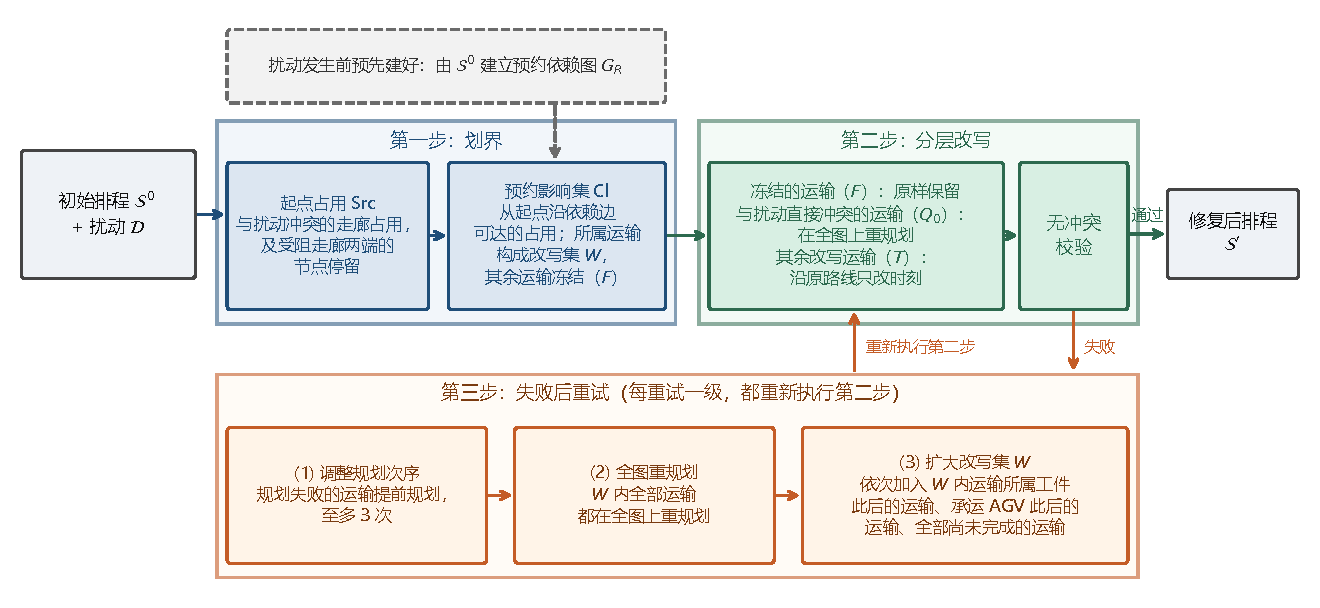
\includegraphics[width=\linewidth]{figures/fig_strc_framework_CN_new}
\caption{分层有界修复的三步流程（B 类扰动）。
顶部虚线框：依赖图只取决于初始排程，在扰动到来前离线建好。
第一步由起点占用沿依赖边得到预约影响集，确定改写集 \(W\) 与冻结的运输 \(F\)；
第二步只改写 \(W\) 内的运输，校验通过即输出修复后的排程；
第三步在校验失败时依次放宽，每放宽一级都重新执行第二步。}
\Description{流程图。左侧输入为初始排程与扰动，顶部虚线框表示离线建好的依赖图。
第一步划界：由与扰动冲突的起点占用，沿依赖边得到预约影响集，其所属运输构成改写集，其余运输冻结。
第二步分层回放：冻结的运输原样保留，与扰动直接冲突的运输在全图上重规划，其余改写运输沿原路线只改时刻，然后做无冲突校验，通过则输出修复后排程。
第三步失败后放宽：依次调整次序重试、令改写集内全部运输在全图上重规划、按同一工件此后的运输、同一 AGV 此后的运输、全部尚未完成运输的顺序扩大改写集，
每一级都重新执行第二步。}
\label{fig:framework}
\end{figure}

\subsection{划界：预约影响集}
\label{sec:closure_def}

\begin{definition}[预约依赖图]
\label{def:dep}
顶点为 \(R\) 中的走廊占用；走廊阻断时，另含受阻走廊两端节点上的停留。
有向边 \(r\to r'\) 表示：\(r\) 一旦改写，\(r'\) 可能也必须改写。边分四类（直观含义见第~\ref{sec:two_graphs}~节）：
\begin{enumerate}[leftmargin=1.4em,itemsep=0.15em]
\item \textbf{让行边：} 同一走廊（或同一节点）、不同 AGV 的两条占用，时间重叠或首尾相接（\(r.t^e=r'.t^s\)），
由进入时刻较早者指向较晚者；在容量大于 \(1\) 的节点上，两条停留重叠时，只有重叠期间该节点曾经停满才连边；
\item \textbf{同车边：} 同一 AGV 按时间先后相邻的两条占用，前一条指向后一条；
\item \textbf{同工件边：} 同一工件工序 \(i\) 的运输占用指向该工件下一道有运输占用的工序的运输占用；
\item \textbf{同机边：} 同一机器上相邻加工的两道工序，前一道的运输占用指向后一道的运输占用。
\end{enumerate}
由此得到 \(G_R\)。
\end{definition}

四类边的示意见图~\ref{fig:graphs}(b)。首尾相接的两条占用在排他语义下并不冲突，
但前一条一旦延后，后一条就必须让路，因此也连让行边。
节点未停满时，两车同时停留互不妨碍，故容量大于 \(1\) 的节点只在停满时连让行边。
受阻走廊两端以外的节点停留不作顶点：节点上的让行由分层回放中的路径规划模块在规划时处理，划界只沿上述边传递。
边集是一种建模选择：它可能多纳入不必改写的占用，也可能漏掉未建模的依赖（注~\ref{rem:minimality}）。

\begin{definition}[预约影响集与时空预约闭包]
\label{def:strc}
给定起点集 \(S\) 与时刻 \(t_{\mathrm{now}}\)，记决策时刻尚未结束的占用为
\[
R^{\circ}=\bigl\{\,r:\ r.t^e>t_{\mathrm{now}}\,\bigr\},
\]
令 \(G_R^\circ\) 为只保留 \(R^{\circ}\) 中的占用及它们之间的边所得的子图。预约影响集定义为
\[
\mathrm{Cl}(S)
=\bigl\{\,v\in R^{\circ}:\
   \exists\,s\in S\cap R^{\circ}\ \text{使}\ s\!\to^*\!v\ \text{于}\ G_R^\circ\,\bigr\},
\]
即从尚未结束的起点出发，沿边可达的全部尚未结束的占用（含起点自身）。
计算 \(\mathrm{Cl}(S)\) 的过程称为时空预约闭包（\STRC）。
\end{definition}

划界即从起点集 \(\mathrm{Src}(\mathcal{D})\) 出发，在 \(G_R^\circ\) 上做一次广度优先搜索，
耗时为 \(O(|R^{\circ}|+|E_R^{\circ}|)\)，其中 \(E_R^{\circ}\) 为 \(G_R^\circ\) 的边集。
依赖图的主体只取决于初始排程 \(\mathcal{S}^0\)：走廊占用之间的四类边在 \(\mathcal{S}^0\) 确定时、扰动到来之前即可\emph{离线}建好。
扰动到来后，\emph{在线}只需把受阻走廊两端节点上的停留接入图中（连出它们的让行、同车、同工件与同机边），再做一次搜索。
本文报告的修复耗时包含在线的接入与搜索，不含离线建图；离线建图在主批次 \(\NPairs\) 对上的耗时中位数为 \(1.2\)\,ms、最大 \(2.9\)\,ms。

图~\ref{fig:closure} 用一个小例子说明这一构造。

\begin{figure}[tbp]
\centering
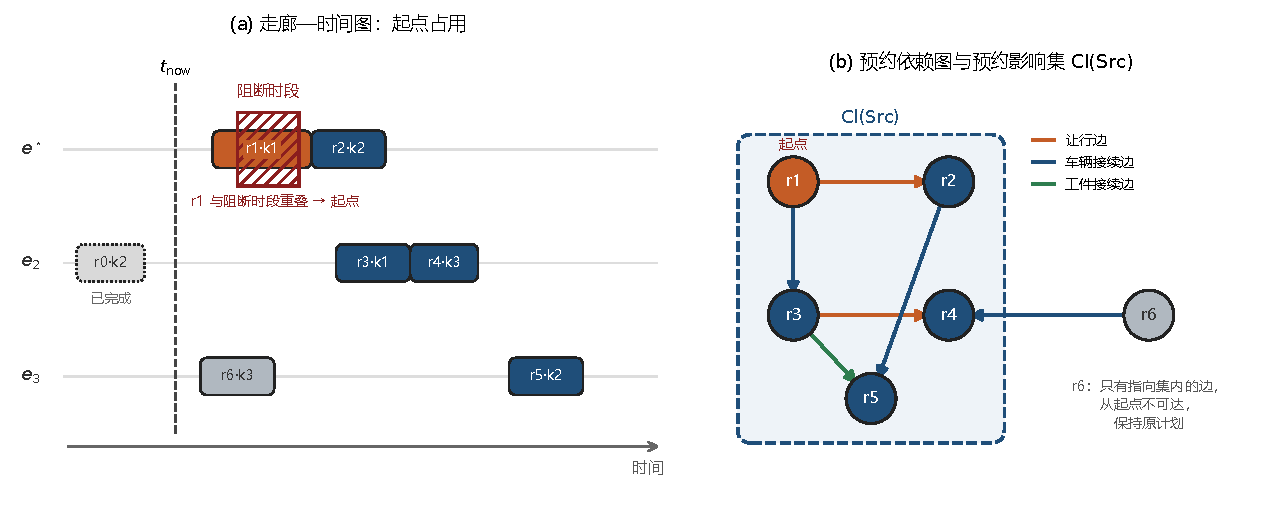
\includegraphics[width=\linewidth]{figures/fig_strc_closure_CN}
\caption{预约影响集的构造示意（同一组占用画在两幅中）。
(a)~走廊—时间图：每个色块是一条走廊占用，标注为「占用·AGV」；
只有 \(r_1\) 与走廊 \(e^\star\) 的阻断时段重叠，成为起点；\(r_0\) 在 \(t_{\mathrm{now}}\) 前已完成，不参与划界。
(b)~这些占用之间的依赖边（颜色区分类型）：从 \(r_1\) 出发沿边可达 \(r_2\)--\(r_5\)，
它们与 \(r_1\) 构成预约影响集 \(\mathrm{Cl}(\mathrm{Src})\)（虚线框）。
让行边只连同一走廊上时段重叠或首尾相接的前后占用，故 \(e_2\) 上的 \(r_3\to r_4\) 连边，而 \(e_3\) 上相隔较远的 \(r_6\)、\(r_5\) 不连边；
\(r_3\) 与 \(r_5\) 运送同一工件的相邻两道工序，以同工件边相连；本例不含同机边。
\(r_6\) 只有指向集内的边，从起点不可达，留在集外并保持原计划；集内没有指向集外的边。
为突出走廊上的传递，本图未画节点停留。}
\Description{左右两幅。左幅是走廊—时间图，三条横线分别是走廊 e-star、e2、e3，
横轴为时间，竖虚线为决策时刻。e-star 上的斜纹框是阻断时段，橙色占用 r1（AGV k1）与之重叠，标为起点；
e2 上最左侧的灰色占用 r0 已在决策时刻前完成。右幅是同一组占用的依赖图：
r1 经让行边指向 r2、经同车边指向 r3，r3 经让行边指向 r4、经同工件边指向 r5，r2 经同车边指向 r5；
r1 到 r5 被虚线框圈为预约影响集。框外的灰色占用 r6 只有一条同车边指向框内的 r4，
标注为从起点不可达、保持原计划。}
\label{fig:closure}
\end{figure}

\textbf{改写集与冻结集。}
路径规划模块一次为一次运输规划完整轨迹，无法只替换其中某几条占用，因此划界的结果以运输为单位使用：
\[
W=\tau\bigl(\mathrm{Cl}(\mathrm{Src})\bigr)
\]
称为\emph{改写集}，\(W\) 内运输在 \(t_{\mathrm{now}}\) 之后的占用都允许改写（已开始的走廊占用除外，假设 A2）；
其余尚未完成的运输构成\emph{冻结集} \(F\)，原样保留。
按占用计，实际允许改写的集合 \(U^{+}\supseteq\mathrm{Cl}\) 为 \(W\) 内运输的全部尚未结束的占用。
同一运输的各条占用由同车边依次相连，排在 \(\mathrm{Cl}\) 内占用之后的已经在 \(\mathrm{Cl}\) 中，
故补齐只会纳入同一运输中排在其前、尚未结束的占用。
在第~\ref{sec:e3}~节的 \(\NPairs\) 对上，\(U^{+}\) 在 \(\SegExtraPairs\) 对上比 \(\mathrm{Cl}\) 多出占用，平均多 \(\SegExtraMean\) 条、最多 \(\SegExtraMax\) 条；
\(U^{+}\) 平均占尚未结束占用的 \(\SegShare\)，\(\mathrm{Cl}\) 为 \(\ClosureShareMean\)。

按工序依赖图划界的对照方法取 \(U\) 为 \(T_{\mathrm{impact}}\) 中各工序在 \(t_{\mathrm{now}}\) 时尚未结束的运输占用；
由命题~\ref{prop:miss}，B 类扰动下这一集合为空。本文方法取 \(U=\mathrm{Cl}(\mathrm{Src})\)。
实验中二者分别记为 AOR 与 \STRC{}。

\subsection{预约影响集的性质}
\label{sec:containment}

\begin{prop}[结构闭合性]
\label{prop:struct}
对任意起点集 \(S\)，在 \(G_R^\circ\) 中不存在边
\(u\to v\) 满足 \(u\in\mathrm{Cl}(S)\) 且 \(v\in R^{\circ}\setminus\mathrm{Cl}(S)\)。
因而，从 \(\mathrm{Cl}(S)\) 出发沿边无法到达影响集外、尚未结束的占用。
\end{prop}

\begin{proof}
若存在这样的边 \(u\to v\)，则由 \(u\in\mathrm{Cl}(S)\) 知存在尚未结束的起点 \(s\) 使
\(s\to^* u\)。拼接 \(u\to v\) 得 \(s\to^* v\)，故按定义~\ref{def:strc} 应有
\(v\in\mathrm{Cl}(S)\)，矛盾。
\end{proof}

命题~\ref{prop:struct} 是定义的直接推论：边集一经固定，影响集对这些边就是封闭的。
它是否覆盖了物理上真实存在的全部依赖，取决于边集的选取，见下面的注。

\begin{remark}[预约影响集与最小允许改写集合]
\label{rem:minimality}
闭合性只说明集内占用没有指向集外的依赖边；它既不保证影响集足以恢复可行，也不说明影响集已经足够小。
下面分三点说明。

其一，\textbf{最小允许改写集合依赖于所用的修复程序，而预约影响集不依赖}。
说集合 \(U\) 最小，必须先指明「在何种修复能力下 \(U\) 足以恢复可行」：允许改派与改序时的最小 \(U\)，
与只允许改路时的最小 \(U\) 不是同一个集合。预约影响集由 \(G_R\) 唯一确定，与修复程序无关，
因此它不能、也不打算等于某一种修复程序下的最小集合。

其二，\textbf{四类边会多纳入不必改写的占用；已知的漏纳情形（首尾相接）已并入让行边}。
让行边只要两条占用重叠就连边，并不判断后者是否\emph{真的}只能等前者通过——若该处另有旁路，
后者改道即可，本不必纳入改写；同车边也可能把延误传不到的链尾一并纳入。这两处使影响集偏大。
为检验首尾相接这一处理是否到位，本文做\emph{差分试探}：在与第~\ref{sec:e3}~节相同的 \(\NPairs\) 对算例上，
将影响集内的每条走廊占用单独延后 \(1\) 个时间单位、其余不变，检查它是否与影响集之外同一走廊上的某条占用新产生时段重叠。
每出现一次计为一次泄漏，即当前边集没有连出、但延后后会发生冲突的依赖。
泄漏总数为 \ProbeLeaks，出现泄漏的对数为 \ProbeLeakPairs；其中 \ProbeOutsidePairs\ 对的影响集外仍有占用，
其余各对的影响集已包含全部尚未结束的占用。首尾相接引起的泄漏为 \(0\)；这 \ProbeLeaks\ 次泄漏都出自两条占用之间留有不足 \(1\) 个时间单位空隙的情形：
延后 \(1\) 个时间单位即与后者重叠，而让行边只连重叠或首尾相接的占用。
这一检验只针对首尾相接这一已知漏边，并不证明边集完备；修复中这类依赖由回放与校验兜住（命题~\ref{prop:outside} 的前提 (iii)）。

其三，\textbf{影响集只界定\emph{允许}改写的范围，不等于\emph{必须}改动的范围}。
集内多数运输并不需要换路线：前车延后时，后车往往沿原路线晚一些出发即可。
在第~\ref{sec:cheap}~节的算例上（繁忙走廊整段阻断），全部尚未完成的运输中，修复后路线改变的只占 \WCRouteFrac，
只改时刻的占 \WCTimeFrac；阻断缩短为 \(5\) 个时间单位时，两者分别为 \(0.05\) 与 \(0.66\)。分层回放正是利用这一点（命题~\ref{prop:must}）。

因此，本文给出的是由结构唯一确定、可复现、对依赖边封闭的允许改写集合；
逼近最小允许改写集合是另一个问题，留作未来工作（第~\ref{sec:limitations}~节）。
\end{remark}

\textbf{影响集的规模。}
\label{sec:structure}
预约影响集由 \(G_R\) 唯一确定，没有可调参数，其规模只能实测。实测上它并不小：
走廊阻断下平均覆盖尚未结束占用的约 \ClosureAliveFrac（第~\ref{sec:e6}~节）；
算例从 \(8\times4\times4\) 放大到 \(\ScaleJobsHi\times\ScaleMachHi\times\ScaleMachHi\) 时，
这一比例在 \ScaleCloAliveLo--\ScaleCloAliveHi\ 之间，没有随规模上升（第~\ref{sec:instscale}~节）。
因此「有界」指范围由依赖关系确定、可以测量；
修复耗时短，一是因为不重新启动搜索，二是因为影响集内只有重规划集需要在全图上搜索（第~\ref{sec:level1}~节）。

影响集的规模由排程与路网共同决定，单看路网无法预测：实验考察了只由路网算出的指标
（毛坯库最小割与漏斗占比），在外部路网上这些指标取值恒定，而同一张路网换用不同机器配置时，
影响集占比明显变化（第~\ref{sec:e4}~节）。

\subsection{B 类扰动的修复：分层回放}
\label{sec:level1}

改写集 \(W\) 内的运输都允许改写，但并非都必须改路线。按与扰动的关系，把尚未完成的运输分为三层。

\begin{definition}[重规划集、平移集与冻结集]
\label{def:tiers}
记 \(Q_0=\tau(\mathrm{Src}_E)\) 为\emph{重规划集}，即走廊起点所属的运输；
\(T=W\setminus Q_0\) 为\emph{平移集}；其余尚未完成的运输构成\emph{冻结集} \(F\)。
改路时，\(Q_0\) 内的运输在全图上重新规划；\(T\) 内的运输先只在原路线所经走廊构成的子图上重新规划，
即路线不变、只改各走廊的进入时刻与节点上的等待，在该子图上找不到可行轨迹时才改在全图上规划，下称\emph{升级}；
\(F\) 内的运输原样保留。
\end{definition}

\begin{prop}[必须改动的运输]
\label{prop:must}
设 \(\mathcal{D}\) 为走廊阻断或通行变慢，\(\mathcal{S}'\) 为满足假设 A2（已开始的行程不回溯）的任一可行修复。
则对每个 \(u\in Q_0\)，\(\mathcal{S}'\) 中运输 \(u\) 的承运 AGV、所经走廊或各走廊的进入时刻至少有一项与 \(\mathcal{S}^0\) 不同。
因而任一可行修复至少改动 \(|Q_0|\) 次运输。
\end{prop}

\begin{proof}
任取 \(u\in Q_0\)，按定义它有一条占用 \(r\in\mathrm{Src}_E\)。
走廊阻断时，\(r\) 与生效时段 \([t_a',t_b)\) 重叠；生效时段始于该走廊上进行中占用的结束时刻之后，
故 \(r\) 在 \(t_{\mathrm{now}}\) 时尚未开始，按假设 A2 允许改写。
若 \(\mathcal{S}'\) 中 \(u\) 的承运 AGV、所经走廊与进入时刻都与 \(\mathcal{S}^0\) 相同，则 \(r\) 原样出现在 \(\mathcal{S}'\) 中，
与阻断时段在同一排他走廊上重叠，\(\mathcal{S}'\) 不可行，矛盾。
通行变慢时，\(r\) 尚未开始且与受扰时段重叠，按原时刻进入后其通行须按倍率加长，
\(\mathcal{S}^0\) 中的离开时刻已不可能实现，同样矛盾。
\end{proof}

命题~\ref{prop:must} 说明 \(Q_0\) 是\emph{必须改动}的运输，\(|Q_0|\) 是改动次数的下界，而不是改路线次数的下界：
\(Q_0\) 内的运输也可能只需推迟出发。
节点起点 \(\mathrm{Src}_V\) 不计入 \(Q_0\)：受阻走廊端点上的停留与阻断时段重叠，并不使原排程不可行，
停在那里的车完全可能不受影响，其运输归入平移集，需要时在改路中升级。
分层的依据是：\(Q_0\) 内的运输必须改动，最可能需要换路线，故直接在全图上搜索；
\(T\) 内的运输只因依赖边被牵连，多数只需平移时刻，在原路线子图上搜索的状态数小得多；
\(F\) 内的运输不受影响，原样保留。
实验中，\(Q_0\) 加上升级的运输占 \(W\) 的比例，在繁忙走廊整段阻断下平均为 \TierReplanShare，阻断缩短为 \(5\) 个时间单位时降为 \(0.15\)；
主批次上升级的运输不到 \(W\) 的 \(1\%\)，分层回放失败而须改为全图重规划的情形没有出现；
规模批次（第~\ref{sec:ablation}~节）上升级约占 \(W\) 的 \(0.2\%\)--\(0.3\%\)，改为全图重规划的只有 \(1\) 对。

给定 \(W\) 与 \(Q_0\)，分层回放（算法~\ref{alg:replay}）分五步：
\begin{enumerate}[label=(\arabic*),leftmargin=2em,itemsep=0.15em]
\item 把扰动写入预约表：阻断按生效时段写入阻断时段，通行变慢则把受扰时段内的通行时间按倍率加长。
\item 新建一张空预约表，先把冻结集 \(F\) 的全部占用、以及 \(W\) 内运输已经开始的走廊占用按原字段原样写回，下称\emph{预提交}。
节点停留随运输走：\(F\) 内运输的停留原样保留；若结束这段停留的下一次出发属于 \(W\) 且尚未发生，该停留的终点留待重规划后的出发确定。
\item 先规划出发状态在 \(t_{\mathrm{now}}\) 已确定的运输：AGV 已载货、或正在离场与驱离途中的，不再依赖任何工件的就绪时刻。
否则，按加工顺序先轮到的运输会按原时刻占住节点，而阻断可能使这些车走不了。
\item 按原加工顺序，逐个为 \(W\) 内其余运输调用路径规划模块（第~\ref{sec:reservation}~节）：
从承运 AGV 在 \(t_{\mathrm{now}}\) 或其上一次运输结束时所在的节点出发，按定义~\ref{def:tiers} 在全图或原路线子图上搜索，
把新占用写回表中，并更新相应机器的空闲时刻与工件的就绪时刻。
需要驱离时，只允许驱离本次修复中新停下的车，或下一次运输属于 \(W\) 的车；要驱离 \(F\) 内运输停放的车，本遍即告失败。
\item 做一次独立校验：无冲突、无占用落入阻断时段、\(F\) 内运输的字段没有被改动。
\end{enumerate}
这一步不改机器指派、不改加工顺序、不换车，只改 \(W\) 内运输的轨迹与时刻。

\begin{algorithm}[t]
\caption{分层回放 \(\textsc{LayeredReplay}\)}
\label{alg:replay}
\begin{algorithmic}[1]
\Require 排程 \(\mathcal{S}^0=(x,\pi,y,R)\)，扰动 \(\mathcal{D}\)，改写集 \(W\)，重规划集 \(Q\subseteq W\)，时刻 \(t_{\mathrm{now}}\)
\Ensure 排程 \(\mathcal{S}'\) 或失败
\State 将 \(\mathcal{D}\) 写入预约表与路网
  \Comment{阻断：按生效时段写入；通行变慢：受扰时段内通行时间按倍率加长}
\State 取空表 \(R'\)
\For{\(F=\) 不在 \(W\) 内的运输，以及 \(W\) 内已开始的走廊占用}
  \State 将原字段预提交到 \(R'\)
    \Comment{已开始的占用必须原样写入，遗漏即等于改写它们}
  \If{与阻断时段冲突}
    \State \Return 失败
      \Comment{起点未覆盖与阻断时段重叠的占用}
  \EndIf
\EndFor
\For{\(W\) 内每个运输 \(u\)：先出发状态已确定者，再按原加工顺序}
  \State 从承运 AGV 的当前状态出发
  \If{\(u\in Q\)}
    \State 在全图上调用路径规划模块
  \Else
    \State 在 \(u\) 原路线的走廊子图上调用路径规划模块；失败则撤销并改在全图上调用 \Comment{升级}
  \EndIf
  \If{无可行轨迹，或须驱离 \(F\) 内运输停放的车}
    \State \Return 失败（记下 \(u\)）
  \EndIf
  \State 提交新占用；按 \(\pi\) 更新相应机器的空闲时刻与工件的就绪时刻
\EndFor
\State 独立校验：无冲突、无占用落入阻断时段、通行变慢时受扰时段内通行时间已按倍率加长、\(F\) 的字段未改
\If{校验通过}
  \State \Return \(\mathcal{S}'=(x,\pi,y,R')\)
\Else
  \State \Return 失败
\EndIf
\end{algorithmic}
\end{algorithm}

按复杂度，划界只需一次广度优先搜索（定义~\ref{def:strc}）；一次 \(\textsc{LayeredReplay}\)
要为 \(W\) 内每个运输各调用一次路径规划模块，耗时主要来自后者。
路径规划模块一次调用的代价随所搜子图的走廊数增长，原路线子图只含该运输原来经过的几条走廊，
因此平移集内运输的搜索比全图搜索小得多。改路过程不启动任何种群搜索。
第~\ref{sec:e3}~节的对照固定回放程序，只替换允许改写范围的来源（工序依赖图或预约影响集），
这样两种划界方法可行率的差别只能来自划界对象。

\begin{prop}[冻结集不变的充分条件]
\label{prop:outside}
设按算法~\ref{alg:replay} 执行分层回放，且满足：
(i)~阻断时段已写入预约表；(ii)~\(F\) 内运输的每条尚未结束的占用都已按原字段预提交到新预约表，且预提交成功；
(iii)~路径规划模块只为 \(W\) 内的运输规划，驱离只针对本次修复中新停下的车或下一次运输属于 \(W\) 的车；
(iv)~最终排程通过无冲突校验。
则在恢复后的预约表 \(R'\) 中，\(F\) 内运输的每条走廊占用的走廊、时段与 AGV 都与 \(\mathcal{S}^0\) 一致；
其节点停留除下述一种情况外也都一致：若结束某段停留的下一次出发属于 \(W\)，该停留的终点随重规划后的出发改变。
\end{prop}

\begin{proof}
由 (ii)，\(F\) 的每条占用在回放开始前已按原区间写入新表，且没有与阻断时段冲突（否则预提交失败）。
由 (iii)，回放只为 \(W\) 内的运输提交新占用，不删除也不改写已提交的占用；
驱离只缩短被驱离车的停留，而按 (iii) 被驱离的车，其停留要么是本次修复新写入的，要么终点本就由 \(W\) 内的出发确定。
因此 \(F\) 的每条走廊占用在新表中的 \((e,[t^s,t^e),k)\) 与预提交值相同，即与 \(\mathcal{S}^0\) 相同。
(iv) 的校验只排除新占用与已有占用之间的冲突，不改变已提交的字段。
\end{proof}

前提 (i)--(iv) 是回放程序自身的执行条件，可在实现中逐条检查；此外，命题还依赖假设
A1（初始排程可行，否则冻结集的原字段之间就可能互相冲突、预提交必然失败）、
A2（已开始的行程不回溯）与 A4（走廊排他、节点限容）。
命题对重规划集与平移集一视同仁：分层只决定 \(W\) 内运输在多大的子图上搜索，不改变 \(F\) 的处理。

\begin{remark}[命题~\ref{prop:outside} 的前提在何种情况下不成立]
\label{rem:precommit}
有三种情况。
第一，预提交失败：若 \(F\) 内某条占用与阻断时段重叠，前提 (ii) 不成立，
说明起点集没有覆盖全部与阻断时段重叠的占用，即起点集不完备。
第二，范围扩展：若改路失败并触发第~\ref{sec:scope_escalation}~节的范围扩展，
改写集变为 \(W'\supsetneq W\)，命题只对最终仍在冻结集中的运输成立。
范围扩展意味着优先保证可行，而不是保证改写最少；发生范围扩展的情况在实验中单独报告。
第三，实现粒度过粗：前提 (iii) 要求路径规划模块\emph{只}为 \(W\) 内的运输规划。
若实现以比单次运输更粗的单位（例如整道工序链、整辆车的后续行程）决定是否改路，\(F\) 内的占用会被一并改写，
命题的结论随之不成立。粒度还须细到走廊：对跨越 \(t_{\mathrm{now}}\) 的运输，已开始的走廊占用原样保留，
改路从 AGV 驶完当前走廊后所在的节点开始；否则会改写已开始的占用，违反假设 A2。
由于这些占用所属的运输在 \(W\) 内，冻结集的比对检查不出这种改写，故另行逐条核对（第~\ref{sec:e2}~节）。
\end{remark}

\subsection{B 类扰动的修复：失败后放宽}
\label{sec:scope_escalation}

分层回放可能失败：在冻结集固定、平移集多沿原路线的前提下，某次运输找不到可行轨迹，
或者它需要驱离冻结集内的车。此时按下列顺序放宽，每一步仍是一遍确定性的分层回放：
\begin{enumerate}[label=(\alph*),leftmargin=2em,itemsep=0.15em]
\item \textbf{调整次序重试。} 记下规划失败的运输；若它的出发位置与工件就绪时刻在 \(t_{\mathrm{now}}\) 已经确定，
下一遍把它提到第 (3) 步与已确定的运输一起先规划，使它先于按加工顺序轮到的运输占用车位。
同一 \(W\) 内至多重试三次。
\item \textbf{全图重规划。} 分层回放连同重试仍失败时，令 \(W\) 内全部运输都在全图上重规划（即取 \(Q=W\)），同样至多重试三次。
\item \textbf{范围扩展。} 仍失败时按下列顺序扩大 \(W\)，每扩大一次就重新执行 (a)(b)，最多三轮：
\begin{enumerate}[label=(\roman*),leftmargin=1.6em,itemsep=0.1em]
\item 加入同一工件此后的运输：当前 \(W\) 内各运输所属工件此后的全部运输；
\item 加入同一 AGV 此后的运输：当前 \(W\) 内各运输的承运 AGV 此后的全部运输；
\item 纳入全部尚未完成的运输，这正是对照方法 UR 的允许改写范围（第~\ref{sec:vs_r0}~节）。
\end{enumerate}
扩大后重规划集 \(Q_0\) 不变，新纳入的运输进入平移集。
\end{enumerate}
实验中触发范围扩展的情形很少：扰动规模扫描的 \(100\) 次运行中触发 \(2\) 次，都在第三级恢复可行（第~\ref{sec:scale}~节）；
算例规模扫描的 \(\ScalePairs\) 对中触发 \(2\) 对，扩到全部仍不可行——UR 在这 \(2\) 对上同样失败，失败来自回放本身而非 \(W\) 过小（第~\ref{sec:instscale}~节）；
主批次阻断缩短为 \(5\) 与 \(2\) 个时间单位时，首轮失败的各 \(2\) 对都在第三级恢复可行（第~\ref{sec:boundary}~节）。
凡经扩展恢复可行的对都走到了第三级，第一、二级从未单独奏效。
第~\ref{sec:e3}~节为比较两种划界的可行率，关闭了范围扩展。

失败后逐步扩大范围的做法已有先例。Local Rescheduling~\cite{kuster2007local}
按时间窗逐步放宽直至可行；AOR 则按工件先后与同机先后纳入后续工序
（第~\ref{sec:rw_aor}~节）。本文先放宽搜索的子图与次序，再沿预约依赖的方向扩大 \(W\)，而不是沿时间窗。
这一步保证影响集过紧时仍能恢复可行，而不必立即转为全局搜索。
算法~\ref{alg:strc_repair} 把三步合起来写出，与图~\ref{fig:framework} 对应。

\begin{algorithm}[t]
\caption{分层有界修复（划界 + 分层回放 + 失败后放宽）}
\label{alg:strc_repair}
\begin{algorithmic}[1]
\Require 排程 \(\mathcal{S}^0\)，扰动 \(\mathcal{D}\)，时刻 \(t_{\mathrm{now}}\)；离线建好的依赖图
\Ensure 排程 \(\mathcal{S}'\) 或失败
\State \(\mathrm{Src}\gets\mathrm{Src}_E\cup\mathrm{Src}_V\)；把 \(\mathrm{Src}_V\) 接入依赖图
\State \(W \gets \tau(\mathrm{Cl}(\mathrm{Src}))\)；\(Q_0\gets\tau(\mathrm{Src}_E)\)
\For{轮次 \(=0,1,2,3\)}
  \For{\(Q\in\{Q_0\cap W,\ W\}\)} \Comment{先分层，再全图}
    \State \(E\gets\varnothing\)
    \Repeat
      \State \(\mathcal{S}' \gets \textsc{LayeredReplay}(\mathcal{S}^0,\mathcal{D},W,Q,t_{\mathrm{now}})\)，其中 \(E\) 内运输先规划
      \If{\(\mathcal{S}'\) 可行}
        \State \Return \(\mathcal{S}'\)
      \EndIf
      \State 把失败的运输加入 \(E\)（若其出发状态已确定）
    \Until{\(E\) 未增加或 \(|E|>3\)}
  \EndFor
  \State 按范围扩展的规则扩大 \(W\) \Comment{工件后缀 / 同车后缀 / 全部尚未完成}
\EndFor
\State \Return 失败
\end{algorithmic}
\end{algorithm}

\subsection{A 类扰动的修复：换车与改派}
\label{sec:afault}

AGV 故障与机器故障直接使 AGV 或工序不可用，只改路不足以恢复，因此另设两项动作（假设 A5：允许的恢复动作）：
\begin{itemize}[leftmargin=1.5em,itemsep=0.15em]
\item \textbf{AGV 故障}：故障 AGV 走完当前走廊后退出路网（假设 A2），此后的运输由其余 AGV 承担，每次运输按预约表试算，选可最早送达的 AGV；
\item \textbf{机器故障}：故障机器上未完工的工序改派到其余候选机器中加工时间最短的一台。
\end{itemize}
加工顺序 \(\pi\) 始终不变，不重开搜索。
实现上，这两项动作通过从 \(t_{\mathrm{now}}\) 起按原加工顺序重新解码完成：
已经开始的占用预提交、不可改写，只从 \(t_{\mathrm{now}}\) 起排定尚未开始的运输与工序，下称\emph{固定前缀解码}。
由于尚未开始的运输都可重新选车，A 类扰动下的修复\textbf{不以预约影响集限制改写范围}，也不使用分层与范围扩展；
A 类扰动下，预约影响集只用于检验它包含按工序依赖图划出的范围（第~\ref{sec:e6}~节）。


%% =====================================================================
\section{实验}
\label{sec:experiments}
%% =====================================================================

本章用九组实验检验第~\ref{sec:contributions}~节的三项贡献。
实验设置之后，各节按所回答的问题组织。
重调度范围（第~\ref{sec:exp_scope}~节）：E1 检验走廊阻断下按工序依赖图划界是否给出空范围，对应贡献 C1（工序依赖图无法刻画的失效）；E2 检验预约影响集的闭合与集外不变，对应 C2（以预约影响集为重调度范围）。
调度方案的可行性（第~\ref{sec:exp_feas}~节）：E3 在同一回放程序下只替换划界对象，比较恢复可行率，对应 C2 与 C3（毫秒级局部恢复）；E4 把比较推广到四类扰动。
重调度速度与完工时间（第~\ref{sec:exp_speed}~节）：E5 与 E6 分别在秒级与毫秒量级上与其他恢复方法对照，回答有界修复的耗时优势从何而来，对应 C3。
消融（第~\ref{sec:ablation}~节）：E7 分别检验划界与分层的贡献。
规模外推（第~\ref{sec:e8}~节）：E8 从扰动规模与算例规模两个方向外推。
最后一节在 Lyu 等发表的布局上复现 E1、E2、E3 与 E5，并以 E9 探索影响集规模能否由路网结构预测。

\subsection{实验设置}
\label{sec:protocol}

\textbf{算例。}
主批次使用\textbf{五个算例}，规模记为「工件数 \(\times\) 机器数 \(\times\) AGV 数」：
一个 \(3\times3\times2\) 的小例，供逐步核对；一个 \(8\times4\times4\) 的拥堵例；
以及三个 \(8\times4\times4\) 的脊式布局 \texttt{S11}、\texttt{S21} 与 \texttt{S22}；路网见图~\ref{fig:layouts}(a)--(c)。
前两个为手工绘制；后三个由本文的算例生成器产生，生成参数包括拥堵等级、异构度 \(h\) 与柔性度 \(f\)。
脊式布局指一条主干走廊（脊）贯穿机器区，各机器经支线挂在脊上的两个枢纽处；
毛坯库与成品库分居脊的两端，各经一条或两条并行通道接入~\cite{suh2022spine}。
全部运输都要经过进出通道和同一段中段走廊，争用因此集中在这几条走廊上。
拥堵例也是这种布局（图~\ref{fig:layouts}(b)），只是两个枢纽之间只有一段较长的中廊，且挂在同一枢纽上的两台机器之间另有直连走廊。
三个脊式布局的规模、异构度与柔性度相同，唯一的差别是并行通道数。
脊式布局记为 \texttt{S}\(xy\)（Spine），\(x\)、\(y\) 依次为库区进出通道数与中段走廊数：
\texttt{S11} 的进出通道与中段各一条，\texttt{S21} 把两库的进出通道各增为两条，\texttt{S22} 再把中段增为两条。
增删一条通道只改变可同时通过的 AGV 数，不改变路程，因此三者之间预约影响集规模的差异可归因于通道容量，而非问题尺寸。

\begin{figure*}[t]
\centering
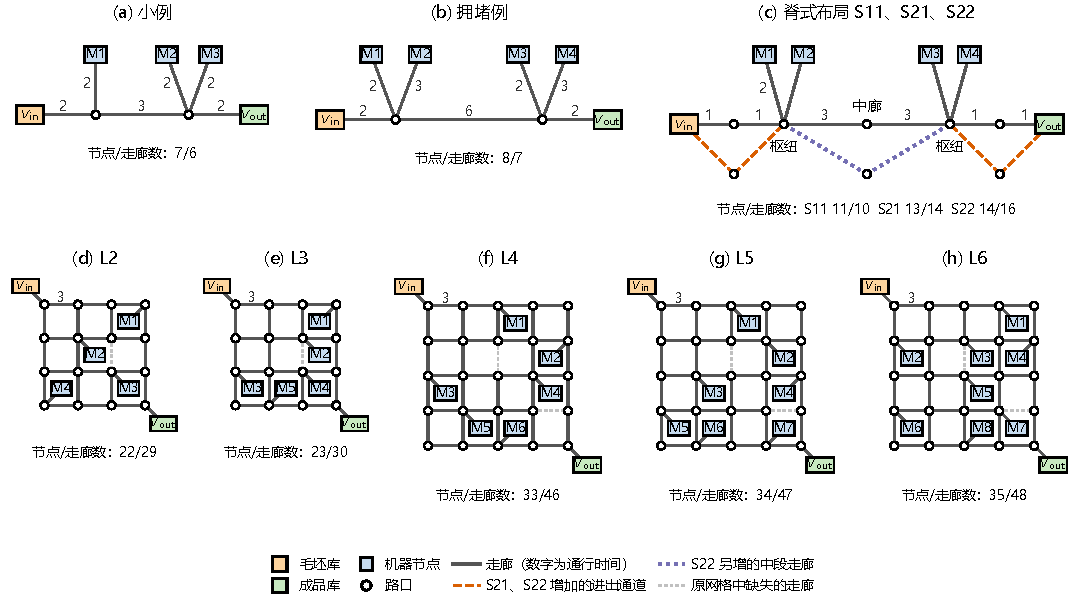
\includegraphics[width=\textwidth]{figures/fig_strc_layouts_CN_new}
\caption{实验所用的路网。上排为主批次：(a)~小例；(b)~拥堵例；(c)~三个脊式布局叠画，实线为 \texttt{S11}，
虚线为 \texttt{S21} 在两库各增加的一条进出通道，点线为 \texttt{S22} 再增加的一条中段走廊；每条并行通道经各自的中间路口，
故增删通道只改容量、不改路程。下排为外部布局批次（Lyu 等~\cite{lyu2019approach} 附录 A 的第 2--6 张布局，记为 \texttt{L2}--\texttt{L6}）：
\texttt{L2}、\texttt{L3} 共用一张 \(4\times4\) 网格，\texttt{L4}--\texttt{L6} 共用一张 \(5\times5\) 网格，灰色虚线为原网格中缺失的走廊，
网格走廊等权（通行时间 \(3\)）。毛坯库 \(v_{\mathrm{in}}\) 与成品库 \(v_{\mathrm{out}}\) 分设，各经一条支线接入；机器节点经支线挂在路口上。
库区不限容量，机器节点容 \(c=3\) 辆，路口容 \(1\) 辆。拓扑逐条读自实验所加载的算例文件。}
\Description{上下两排路网图。上排三幅：小例为毛坯库经两个路口连到三台机器、再接到成品库的小网；拥堵例为两个枢纽之间一段长中廊、
每个枢纽挂两台互相直连的机器；脊式布局从毛坯库经进出通道到近端枢纽，再经中廊到远端枢纽，最后接到成品库，每个枢纽挂两台机器，
虚线和点线分别标出 S21 与 S22 增加的并行通道。下排五幅是 4 乘 4 与 5 乘 5 的网格，毛坯库都在左上角、成品库都在右下角，
机器位于不同的网格节点上，少数网格边以灰色虚线标为缺失。}
\label{fig:layouts}
\end{figure*}

\textbf{随机种子与配对。}
算例生成时的随机种子只决定算例本身，与运行随机种子相互独立。
运行随机种子决定初始排程的加工顺序（见下），从而决定繁忙走廊与阻断时段的位置，也用作 GR 的搜索随机种子。
\textbf{运行随机种子取十个}，均在实验前一次性固定、未按结果挑选，依次为 \(42\)、\(7\)、\(2024\)、\(99\)、\(123\)、\(13\)、\(1\)、
\(777\)、\(31415\) 与 \(8\)；E5 取其中前三个。
五个算例与十个随机种子共组成 \(\NInst\times\NSeeds=\NPairs\) 个算例--随机种子对，下文简称「对」。
全文所有逐对比较、胜负计数与配对检验都以同一算例--随机种子对为单位：
同一对上各方法读取同一份初始解、同一段阻断与同一决策时刻。
初始排程按启发式一次构造，不经搜索优化：
机器指派 \(x\) 为每道工序取加工时间最短的候选机器（并列时取编号小者）；
加工顺序 \(\pi\) 为按运行随机种子随机打乱的工序序列；
按 \(\pi\) 依次排定各工序，每次运输都对每辆 AGV 在当前预约表上实际规划整条轨迹，取送达最早者作为 AGV 指派 \(y\)（并列时取编号小者），
其路径由第~\ref{sec:reservation}~节的路径规划模块写入预约表 \(R\)。
所得排程通过独立无冲突校验；同一算例--随机种子对下各对照方法共享该初始解。
划界只依赖 \(\mathcal{S}^0\) 本身（第~\ref{sec:system_brief}~节），对 \(\mathcal{S}^0\) 只要求其在扰动前可行。
由于 \(\mathcal{S}^0\) 未经优化，可以改动指派与顺序的 GR 有时能把完工时间降到扰动前的 \(C_{\max}(\mathcal{S}^0)\) 以下（第~\ref{sec:scale}~节），
比较完工时间时须考虑这一点。

\textbf{实现与运行环境。}
全部实验为纯 Python 标准库实现，不依赖第三方数值库；下层路网、路径规划模块与独立校验器
为本文自行实现，各对照方法共用同一份代码。单机单线程运行，不使用并行：Intel Xeon W-1270
（\(8\) 核 \(16\) 线程）、\(64\)\,GB 内存、Windows 11，解释器为 CPython \(3.9.6\)（\(64\) 位）。
所有计时结果都在上述单机单线程条件下取得，
更换硬件会使其整体平移，故本文的耗时结论均以\emph{比值}或\emph{量级}形式给出，不依赖绝对毫秒数。

\textbf{外部布局批次。}
上述五个算例（下称\emph{主批次}）的布局均由本文构造。为检验结论是否依赖这几张布局，
另取 Lyu 等~\cite{lyu2019approach} 附录 A 发表的布局运行一批算例，
\textbf{只借用其路网，其余设置与主批次相同}：工件数、AGV 数、每工件工序数、\(h\)、\(f\)
以及运输/加工时长比的标定目标一律不变，随机种子仍取同样十个，因此两批结果之差只能来自布局本身。

路网的网格尺寸、装货站与卸货站以及各机器所在节点、网格中哪些相邻节点之间没有走廊，均逐项转录自原文布局图，
再与 van Os 工具集所附的机读编码逐项核对。附录共六张布局（下称 \texttt{L1}--\texttt{L6}，L 取自 Lyu，编号沿用原文，依次含 \(3\) 至 \(8\) 台机器）；
\texttt{L1} 只有 \(3\) 台机器，在 \(f=0.6\) 下每道工序平均只有 \(1.8\) 台候选机器，
达不到「每道工序至少两台候选机器」的要求，故未采用。
其余五张共 \NPubInst\ 个算例、\NPubPairs\ 个算例--随机种子对，但只落在 \NPubNets\ 张网格上：
\texttt{L2}、\texttt{L3} 共用一张 \(4\times4\) 网格，\texttt{L4}--\texttt{L6} 共用一张 \(5\times5\) 网格，彼此只差机器台数与位置（图~\ref{fig:layouts}(d)--(h)）。
因此这批数据在路网形状上只有 \NPubNets\ 个独立样本，在机器配置上有 \NPubInst\ 个，第~\ref{sec:e4}~节按此划分给出论断。

与原文数据相比，本批有三处调整：
(1)~原文附录未给出逐段通行时间，本文按所有走廊等权补齐，因此本批不与 Lyu 或 van Os 报告的数值作比较；
(2)~原文的装货站与卸货站分别取为毛坯库 \(v_{\mathrm{in}}\) 与成品库 \(v_{\mathrm{out}}\)，与第~\ref{sec:shop}~节的设定一致；
机器与两库按第~\ref{sec:reservation}~节的节点模型经支线挂在原网格的节点上，原网格的走廊不变；
(3)~不采用原文的工件数据：公开算例中运输时长只占加工时长的百分之几，走廊争用几乎不出现，
本文要观察的现象无从发生。
van Os 工具集中另有一组布局（Liu 2023）允许 AGV 沿对角线行驶，
与本文只含上下左右走廊的路网模型不同，未纳入。

\textbf{扰动。}
全部实验的决策时刻统一取 \(t_{\mathrm{now}}=0.35\,C_{\max}(\mathcal{S}^0)\)。该值在实验前固定：此时约四成占用已结束、六成尚未结束，
既有须保持不变的已执行部分，也有足够的待修复部分；本文未对该取值做敏感性分析。各实验的扰动如下。
E1--E3 与 E5--E7 阻断一条繁忙走廊，即在 \(t_{\mathrm{now}}\) 时尚未结束的占用最多的走廊；
阻断时段连续，从该走廊上这些占用中最早的开始时刻持续到最晚的结束时刻，因而覆盖它们全部。
下文把这种扰动称为\emph{繁忙走廊阻断}。
E7 另把阻断时长截短为 \(5\) 与 \(2\) 个时间单位（从同一开始时刻起，不超过整段阻断），并在算例规模序列（第~\ref{sec:instscale}~节）上重复。
E4 在同一决策时刻另加三类扰动（第~\ref{sec:e6}~节）。E9 阻断毛坯库最小割中的走廊（第~\ref{sec:e4}~节）。
E8 的扰动规模部分先把在 \(t_{\mathrm{now}}\) 时仍有尚未结束占用的工序，按各自最早一条这类占用的开始时刻排序，
取前 \(\varphi\) 比例作为受扰工序；这些工序的每条尚未结束的占用各自生成一段阻断，阻断的走廊与时段就是该占用本身。
各段阻断不合并为一段长阻断，否则会同时盖住其间未被选中工序的占用。

\textbf{对照方法。}
\label{sec:vs_r0}
对照分两类。一类是秒级的全局重调度 GR，它可改派与改序，因而更可能缩短 \(C_{\max}\)，但算法耗时由预算决定（第~\ref{sec:e5}~节）。
仅与 GR 对照还留下一个问题：在毫秒量级的耗时内，按影响集划界是否必要？
因此另一类是三种不按影响集限制范围、耗时同在毫秒量级的做法（UR、RS、RD），
构成有界修复在\emph{同一耗时量级内}的对照（第~\ref{sec:cheap}~节）。
连同按工序依赖图划界的 AOR，共六种方法，按与本文方法的差别由小到大列出：
\begin{itemize}[leftmargin=1.5em,itemsep=0.2em]
\item \textbf{\STRC{}（本文方法）}：按时空预约闭包得到的预约影响集划界，再做分层回放（第~\ref{sec:level1}~节）。
范围扩展只在 E8 中开启，E1--E3 与 E5--E7 中关闭。
\item \textbf{AOR}（Affected Operations Rescheduling，受影响工序重调度）：按工序依赖图上的影响域划界，再做与 \STRC{} 相同的分层回放，全文取 \(\theta=2\)。
\(\theta\) 是在工序依赖图上向后扩张的最大跳数。本实现只沿工件先后边扩张、不沿同机先后边扩张，
较定义~\ref{def:task_impact} 窄；扩张边与 \(\theta\) 都只影响 A 类扰动下 \(|U_{\mathrm{AOR}}|\) 的大小；
B 类扰动不直接作用于任何工序，起点工序集为空，无论扩张多少跳，结果都是空集（命题~\ref{prop:miss}）。
AOR 与 \STRC{} 只差划界对象。
\item \textbf{UR}（Unbounded Replay，不划界回放）：不按影响集限制范围，取改写集为全部尚未完成的运输；
重规划集与 \STRC{} 相同（走廊起点所属的运输），其余运输同样先沿原路线只改时刻，分层回放程序完全相同，
因而与本文方法只差「改写集取 \(W\) 还是全部尚未完成的运输」这一项，是唯一能单独检验预约影响集作用的对照（第~\ref{sec:cheap}、\ref{sec:boundary}~节）。
E7 的消融另用其不分层的变体 \textbf{RR}（Re-Route，全部重规划）：全部尚未完成的运输都在全图上重规划，不设平移集；RR 与 UR 只差是否分层。
\item \textbf{RS}（Right Shift，全局右移）：不划界也不改路，只把尚未结束的占用整体推到阻断结束之后（第~\ref{sec:cheap}~节）。
\item \textbf{RD}（Re-Decode，原染色体重解码）：染色体不变，按固定前缀解码（第~\ref{sec:afault}~节）一次，是本实现中耗时最短的全局重算（第~\ref{sec:cheap}~节）。
\item \textbf{GR}（Global Rescheduling，全局重调度）：以原排程为起点、在相同禁行约束下、在限定时间内重新搜索。
采用遗传算法，把 \((x,\pi)\) 编码为一条染色体；一次\emph{解码}指：按该染色体的指派与加工顺序，
在已写入阻断时段的预约表上为尚未开始的运输调用路径规划模块，得到新的 \(R\) 与 \(C_{\max}\)。
种群 \(40\)，采用热启动，即把原排程对应的染色体置入初始种群，以免丢掉原排程已有的指派与路径信息；
解码采用与 RD 相同的固定前缀解码，\(t_{\mathrm{now}}\) 之前的占用不可改写。
\emph{不设代数上限与早停阈值}，只按运行时间预算终止，预算取值见第~\ref{sec:e5}~节。
\end{itemize}
五种对照与 \STRC{} 的差别逐级扩大：AOR 只差划界\emph{对象}，UR 只差\emph{是否}划界，
RS 既不划界也不改路，RD 与 GR 重算全局：RD 按原染色体解码一次，GR 在预算内反复搜索。

对照方法 AOR 的划界规则取自第~\ref{sec:rw_aor}~节所述的工序级
局部重调度做法，由本文重新实现。逐条对应关系是：「受影响工序集取直接受扰工序，
再沿工序先后关系向后扩张」这一条划界规则取自
原始 AOR~\cite{subramaniam2003maor}；
而\emph{只沿工件先后边扩张并以跳数 \(\theta\) 截断}、以及\emph{把工序集映射为须释放的走廊预约}
两项由本文写定——原文的设定里没有预约表，这一映射在原文中无对应物；
分层回放部件则与 \STRC{} 共用同一份实现，以保证两者只差划界对象。
因此 AOR 是将该划界规则移植到本文预约设定下的对照，其结果反映该规则在此设定下的表现，
而非原方法在其自身设定下的表现。

\textbf{预算设置。}
各方法不在同一预算下比较：AOR、\STRC{}、RS、RD、UR 均为一次确定性修复，
运行结束即终止，耗时由算例规模与影响集大小决定而非由预算设定；只有 GR 按运行时间预算终止。
因此涉及 GR 的结果都是在给定预算下得到的；其余五种方法都运行一次即终止，彼此可以直接比较。算法耗时按批次报告，不跨批次比较。

\textbf{两批算例的分工。}
E1--E3 要求完全控制运输/加工时长比等决定走廊争用是否成立的参数，公开算例族无法提供这种控制，
故其结论由主批次单独给出。外部布局批次只检验这些结论在 Lyu 等的布局上能否复现（第~\ref{sec:pubrepro}~节），
不产生新的性能对比结论。两批只在两处合并分析：E9 借它区分「指标过粗」与「算例几何差异不足」两种解释；
E5 合并两批只为增加样本量。

\textbf{统计方法。}
推断性检验均在第~\ref{sec:cheap}、\ref{sec:ablation}~节：\STRC{} 与 UR 在改动比例上的差、UR 与 RR 在耗时上的差（各在主批次与规模序列上取三种阻断时长），
以及 \STRC{} 与 RD 在完工时间上的差；耗时按逐对比值的对数检验。均采用 Wilcoxon 符号秩检验，双侧，配对单位为算例--随机种子对，即取同一对上两种方法结果之差；
差值非零的对少于 \(6\) 时不作检验（\STRC{} 对 UR 在主批次整段阻断下即属此类），实际检验共 \(12\) 次。
只有 \STRC{} 对 UR、\STRC{} 对 RD 在主批次整段阻断下的比较是事先确定的；较短阻断、规模序列与 RR 的消融是在看到该结果之后加入的，属于事后补充，
故按 Holm 法对 \(12\) 次检验一并校正，正文与表中报告校正后的 \(p\) 值。
其余各处的逐对胜负、均值与中位数均为\emph{描述性}统计，不作显著性断言。
\STRC{} 与 RD 的差另报 \(95\%\) 自助置信区间（百分位法，\(10^4\) 次重采样，固定随机种子）；离散度按四分位距报告。
其余各批次的表格只给均值、中位与计数，不含区间。

\subsection{重调度范围}
\label{sec:exp_scope}

本节检验两种划界给出的重调度范围：E1 检验走廊阻断下按工序依赖图划界是否为空，E2 检验预约影响集是否对依赖边封闭、修复后集外占用是否保持原计划。

\subsubsection{E1：工序依赖图给出空范围}
\label{sec:e1}

本节检验命题~\ref{prop:miss} 在扩样算例上是否成立。按第~\ref{sec:protocol}~节的设置，
在 \(\NPairs\) 对上各阻断一条繁忙走廊，分别按工序依赖图与按预约影响集划界，并检查阻断后原排程是否仍可行。
结果如表~\ref{tab:e1} 与图~\ref{fig:e1e3}（左）所示。

从表~\ref{tab:e1} 可以看到，命题的三个条件在全部 \(\PassMiss\) 对上同时成立：
按工序依赖图得到的受影响工序集为空（\(T_{\mathrm{impact}}=0\)），起点占用与预约影响集非空，原排程在阻断后不可行。
其中第一条由定义~\ref{def:task_impact} 对 B 类的约定直接得到；有实质内容的是第三条，即原排程\emph{确实}已经不可行。
因此在这些对上，「工序依赖图给出空范围，故无需重调度」这一推断都不成立。

\begin{table}[t]
\centering
\caption{E1 走廊阻断下两种划界给出的范围（每算例 \(\NSeeds\) 个随机种子，共 \(\NPairs\) 对）。
「三条件通过」计命题~\ref{prop:miss} 的三个条件同时成立的算例--随机种子对（\(T_{\mathrm{impact}}=0\)、
起点占用非空、阻断后原排程不可行）。\(|R|\) 为全表走廊占用数，\(|\mathrm{Src}|\) 为走廊起点占用数 \(|\mathrm{Src}_E|\)，
\(|\mathrm{Cl}|\) 为预约影响集中的走廊占用数，\(\mathrm{Cl}/|R|\) 为二者之比；端点停留 \(\mathrm{Src}_V\) 及其在影响集中的节点停留不计入这三列。
均值取 \(\NSeeds\) 个随机种子的平均。
\texttt{S11}、\texttt{S21}、\texttt{S22} 为三个脊式布局，命名规则见第~\ref{sec:protocol}~节。}
\label{tab:e1}
\small
\begin{tabular}{@{}lcccccc@{}}
\toprule
算例 & 随机种子 & 三条件通过 & 均 \(|R|\) & 均 \(|\mathrm{Src}|\)
 & 均 \(|\mathrm{Cl}|\) & \(\mathrm{Cl}/|R|\) \\
\midrule
小例   & 10 & \(10/10\) & \(28.6\)  & \(5.7\)  & \(16.1\) & \(0.56\) \\
拥堵例 & 10 & \(10/10\) & \(96.0\) & \(18.7\) & \(57.7\) & \(0.60\) \\
\texttt{S11}  & 10 & \(10/10\) & \(164.4\) & \(15.2\) & \(92.1\) & \(0.56\) \\
\texttt{S21}    & 10 & \(10/10\) & \(161.8\) & \(14.8\) & \(93.9\) & \(0.58\) \\
\texttt{S22}     & 10 & \(10/10\) & \(161.0\) & \(14.3\) & \(91.5\) & \(0.57\) \\
\midrule
合计 & \(\NPairs\) & \(\PassMiss\) & --- & --- & --- & --- \\
\bottomrule
\end{tabular}
\end{table}

\textbf{影响集占比。}表中还可以看到，\(|\mathrm{Cl}|\) 随算例变大而增大（\(16.1\)、\(57.7\)、\(91.5\)--\(93.9\)），
这是占用总数变多的直接结果。\(\mathrm{Cl}/|R|\) 在五个算例上都落在 \EoneCloLo--\EoneCloHi 之间，
算例之间的差别与同一算例内不同随机种子之间的差别同量级：逐算例的四分位距为 \EoneFracIqrLo--\EoneFracIqrHi，
\(\NPairs\) 对合在一起的中位数为 \EoneFracMed、极差为 \EoneFracMin--\EoneFracMax。

结论：B 类扰动下，按工序依赖图划界得到空范围，而原排程已不可行。

\subsubsection{E2：闭合性与集外不变}
\label{sec:e2}

本节检验预约影响集的两条性质在实验中是否成立。
\textbf{E2a，结构闭合}（命题~\ref{prop:struct}）：没有依赖边从预约影响集内指向集外尚未结束的占用。
这是图上的性质，由定义直接保证，检验的是实现与定义是否一致。
\textbf{E2b，集外不变}（命题~\ref{prop:outside}）：只在影响集内做分层回放后，集外每条占用的走廊、时段与 AGV 都保持原值。
这是修复之后的性质，检验的是该命题的前提在实验中是否满足。

结果如表~\ref{tab:e2} 所示。在全部 \(\NPairs\) 对上，影响集都是封闭的。
只在影响集内做分层回放（不做范围扩展）时，全部 \(\NPairs\) 对都恢复了可行，且集外占用逐条保持原值，即预提交从未失败（注~\ref{rem:precommit}）。
这里的「集外」与命题~\ref{prop:outside} 一致，指改写集 \(W\) 之外，即冻结集 \(F\) 的占用（第~\ref{sec:level1}~节）。
由于跨越 \(t_{\mathrm{now}}\) 的运输在改写集内，E2b 不比对其已开始的走廊占用；为此另行逐条核对 \(t^s<t_{\mathrm{now}}\) 的占用，
全部 \(\NPairs\) 对上均未被改写。

\begin{table}[t]
\centering
\caption{E2 闭合性与集外不变（每算例 \(\NSeeds\) 个随机种子）。E2a：没有依赖边从预约影响集内指向集外尚未结束的占用；
「分层回放可行」：只在影响集内做分层回放、不做范围扩展时恢复可行；
E2b：改写集 \(W\) 之外（冻结集 \(F\)），占用的走廊、时段与 AGV\emph{逐条}不变。\texttt{S11}、\texttt{S21}、\texttt{S22} 的含义见表~\ref{tab:e1}。}
\label{tab:e2}
\small
\begin{tabular}{@{}lccc@{}}
\toprule
算例 & E2a 闭合 & 分层回放可行 & E2b 集外逐条不变 \\
\midrule
小例   & \(10/10\) & \(10/10\) & \(10/10\) \\
拥堵例 & \(10/10\) & \(10/10\) & \(10/10\) \\
\texttt{S11}  & \(10/10\) & \(10/10\) & \(10/10\) \\
\texttt{S21}    & \(10/10\) & \(10/10\) & \(10/10\) \\
\texttt{S22}     & \(10/10\) & \(10/10\) & \(10/10\) \\
\midrule
合计 & \(\PassClosed\) & \(\FeasRtwo\) & \(\PassInvar\) \\
\bottomrule
\end{tabular}
\end{table}

结论：预约影响集对依赖边封闭；只在其内做分层回放即可恢复可行，且集外占用保持原值。

\subsection{调度方案的可行性}
\label{sec:exp_feas}

本节比较修复后能否得到可继续执行的排程：E3 在同一回放程序下只更换划界对象，E4 把比较推广到四类扰动。

\subsubsection{E3：只更换划界对象}
\label{sec:e3}

本节检验：在同一套回放程序下只更换划界对象，恢复可行率是否随之改变。
AOR 与 \STRC{} 使用同一份初始解、同一个决策时刻、同一批随机种子与同一段阻断时段，都只做一遍分层回放，
\textbf{唯一的差别是允许改写哪些占用}。本节关闭范围扩展：若开启，AOR 可在扩大到全部尚未结束的占用后恢复可行，
测得的就不再是划界对象的差别。结果如表~\ref{tab:e3} 与图~\ref{fig:e1e3}（右）所示。

从表~\ref{tab:e3} 可以看到，在全部 \(\NPairs\) 对上，AOR 的允许改写集合都为空而 \STRC{} 非空；
AOR 全部不可行，\STRC{} 全部恢复可行。AOR 的允许改写集合为空时，回放不改动任何占用，
原排程原样保留，仍占用被阻断的走廊。因此，AOR 不可行是因为它判定无需重调度，而不是修复做得不好。
\STRC{} 的耗时（含在线划界）中位数为 \(\MsRepairMed\)\,ms，最大为 \(\MsRepairMax\)\,ms。

\textbf{边权稳健性。}本文的走廊边权取等权，即每条走廊的通行时间相同。为检验上述结果是否依赖这一设定，
另按三种非均匀边权在同一批 \(\NPairs\) 对上重新运行 E1 与 E3：
其一，各走廊通行时间独立乘以对数正态因子（几何均值为 \(1\)）；
其二，离毛坯库 \(v_{\mathrm{in}}\) 越远的走廊越慢，最远处为原来的 \(1.8\) 倍；
其三，各走廊随机取原通行时间的一半或两倍。
三种边权下，E1 的三个条件仍在全部对上成立，AOR 仍全部不可行；
\STRC{} 在三种边权下分别有 \(\WeightLogRtwo\)、\(\WeightLuRtwo\) 与 \(\WeightSplitRtwo\) 对恢复可行（不做范围扩展）；等权时为 \(\FeasRtwo\)。
可见，按工序依赖图划界得到空范围、AOR 无法恢复可行这两点都不随边权改变；\STRC{} 的首轮可行率则受边权影响。

\begin{table}[t]
\centering
\caption{E3 只更换划界对象（不做范围扩展；每算例 \(\NSeeds\) 个随机种子）。
「AOR 空、\STRC{} 非空」计 AOR 的允许改写集合为空而 \STRC{} 非空的算例--随机种子对；末两列为 \(\NSeeds\) 个随机种子的均值。
\texttt{S11}、\texttt{S21}、\texttt{S22} 的含义见表~\ref{tab:e1}。}
\label{tab:e3}
\small
\begin{tabular}{@{}lccccc@{}}
\toprule
算例 & AOR 空、\STRC{} 非空 & AOR 可行 & \STRC{} 可行 & 均 \(|U_{\mathrm{STRC}}|\) & \STRC{} 耗时/ms \\
\midrule
小例   & \(10/10\) & \(0/10\) & \(10/10\) & \(16.1\) & \(1.50\) \\
拥堵例 & \(10/10\) & \(0/10\) & \(10/10\) & \(57.7\) & \(5.51\) \\
\texttt{S11}  & \(10/10\) & \(0/10\) & \(10/10\) & \(92.1\) & \(7.76\) \\
\texttt{S21}    & \(10/10\) & \(0/10\) & \(10/10\) & \(93.9\) & \(8.00\) \\
\texttt{S22}     & \(10/10\) & \(0/10\) & \(10/10\) & \(91.5\) & \(8.14\) \\
\midrule
合计 & \(\NPairs/\NPairs\) & \(\FeasRone\) & \(\FeasRtwo\) & --- & --- \\
\bottomrule
\end{tabular}
\end{table}

\begin{figure}[tbp]
\centering
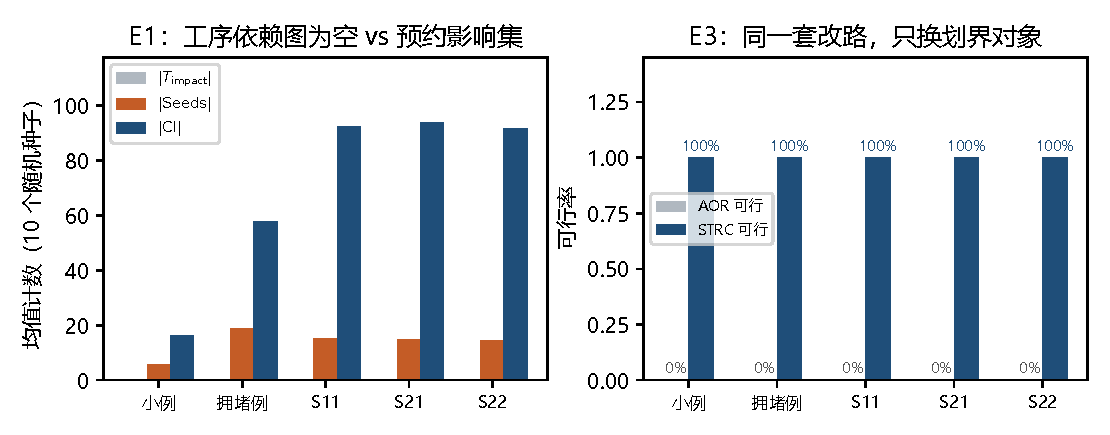
\includegraphics[width=\linewidth]{figures/fig_strc_e1e3_CN_new}
\caption{E1 与 E3 的结果（每算例 \(\NSeeds\) 个随机种子）。
左：每算例按工序依赖图得到的受影响工序数、起点占用数与预约影响集的占用数，柱高为 \(\NSeeds\) 个随机种子的均值；
\(|\mathrm{Cl}|\) 的逐算例四分位距为 \(4\)--\(11\)。
右：一遍分层回放、不做范围扩展时 AOR 与 \STRC{} 的恢复可行率，按算例--随机种子对计数。}
\Description{并排两幅条形图。左幅按五个算例给出工序依赖图影响域、起点占用数与预约影响集规模
三组柱子，影响域一组恒为零，另两组随算例规模上升。右幅给出两种划界的恢复
可行率，按工序依赖图划界一侧为零，按预约影响集划界一侧为百分之百。}
\label{fig:e1e3}
\end{figure}

结论：只替换划界对象，恢复可行率就从 \(\FeasRone\) 变为 \(\FeasRtwo\)。

\textbf{实例。}
\label{sec:case}
\begin{sloppypar}
E1--E3 给出的是 \(\NPairs\) 对上的计数与可行率。为在工序时间轴上直观展示「工序依赖图给出空范围、按预约影响集可以修复」的情形，
图~\ref{fig:case} 给出一个具体例子（选小例是因为其甘特图能逐道工序看清）：
算例为 \(3\times3\times2\) 的小例（\(3\) 个工件、\(3\) 台机器、\(2\) 辆 AGV），运行随机种子为 \(42\)，
扰动为繁忙走廊阻断，其余设置与 E3 相同。
\end{sloppypar}

该例上按工序依赖图得到的受影响工序为空（\(T_{\mathrm{impact}}=\varnothing\)），而走廊起点占用有 \(6\) 条、预约影响集中的走廊占用有 \(16\) 条。
图~\ref{fig:case}(a) 为扰动前原排程的机器甘特图：蓝色工序的运输占用落入影响集（将被重写），
灰色工序在影响集外（预提交、保持原计划）；红色虚线为 \(t_{\mathrm{now}}\)，浅红带为阻断时段。
图~\ref{fig:case}(b) 为修复后：影响集内工序时间轴重排，排程在阻断下恢复可行，
\(C_{\max}:48\to 74\)，耗时约 \(2\)\,ms。
本图只说明局部改动的形态，不用于比较完工时间。

\begin{figure}[tbp]
\centering
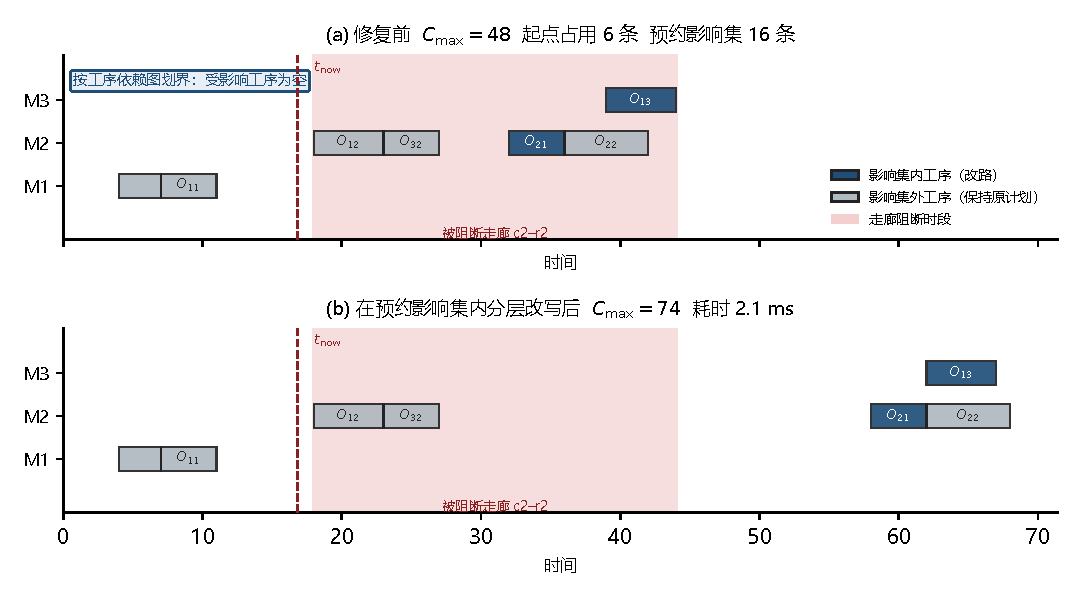
\includegraphics[width=\linewidth]{figures/fig_strc_case_CN_new}
\caption{案例甘特图（\(3\times3\times2\) 小例，运行随机种子 \(42\)，繁忙走廊阻断）。
(a)~阻断前原排程，按是否属于 \(\mathrm{Cl}\) 着色；
(b)~分层回放后。工序依赖图上的影响域为空；蓝色工序对应影响集内运输被重写。
本图仅示意局部改动的形态。}
\Description{上下两幅机器甘特图。(a) 阻断前的原排程，条块按其运输占用是否落在
预约影响集内着蓝灰两色，一条竖直红虚线标出决策时刻，一条浅红竖带标出阻断时段。
(b) 修复后的排程，蓝色条块的时间轴被重排，灰色条块位置不变，完工时间由 48 增至 74。}
\label{fig:case}
\end{figure}

\subsubsection{E4：四类扰动下的划界与修复}
\label{sec:e6}

E1--E3 只考察了走廊阻断一种扰动。本小节检验 E1--E3 的划界与修复结论在其他扰动类型下是否仍然成立：
在同一 \(\NPairs\) 对上另加走廊通行变慢、AGV 故障与机器故障三类。

\textbf{测量内容。} 划界方面，四类扰动均报告工序依赖图上影响域的规模、预约影响集的规模，以及后者是否包含前者。
修复方面，四类扰动均执行修复。B 类仍只做分层回放：阻断时段写入预约表；通行变慢在变慢时段内使该走廊的通行时间加倍，
时段外照常，走廊始终可通行。
A 类额外允许换车或改派，不改变加工顺序；是否扩大允许改写的范围不影响其动作集合。

\begin{table}[t]
\centering
\caption{E4 扰动类型 \(\times\) 划界对象（\(\NPairs\) 对/类，共 \(200\) 次测量）。
通行变慢与阻断的走廊起点占用相同，但通行变慢下走廊仍可通行、车不在走廊口等待，故不取端点停留起点 \(\mathrm{Src}_V\)，其预约影响集包含于阻断的预约影响集。
\(|R^{\circ}|\) 为 \(t_{\mathrm{now}}\) 之后尚未结束的占用数。
「AOR 为空」计按工序依赖图划界判该扰动无需重调度的算例--随机种子对。
末列「修复可行」不做范围扩展：B 类为在预约影响集内做分层回放（\STRC{}）；
A 类为固定前缀解码下的换车或改派（第~\ref{sec:afault}~节），不以预约影响集限制改写范围。}
\label{tab:e6}
\small
\begin{tabular}{@{}llccccc@{}}
\toprule
扰动 & 类 & AOR 为空 & 均 \(|U_{\mathrm{AOR}}|\) & 均 \(|\mathrm{Cl}|\)
 & \(\mathrm{Cl}/|R^{\circ}|\) & 修复可行 \\
\midrule
走廊阻断   & B & \(50/50\) & \(0.0\)  & \(70.3\) & \(0.90\) & \FeasESixBlock \\
走廊通行变慢 & B & \(50/50\) & \(0.0\)  & \(68.4\) & \(0.88\) & \FeasSlow \\
AGV 故障   & A & \(0/50\)  & \(34.9\) & \(58.0\) & \(0.77\) & \FeasESixAgv \\
机器故障 & A & \(0/50\)  & \(45.8\) & \(69.4\) & \(0.91\) & \FeasESixRa \\
\bottomrule
\end{tabular}
\end{table}

结果如表~\ref{tab:e6} 所示，从中可以看到四点。

第一，两类 B 扰动按工序依赖图划界全部为空，两类 A 扰动全部非空，
即 \textbf{A/B 分类在全部 \(200\) 次划界测量上无一例外}。

第二，在全部 \(100\) 次 A 类测量上 \(U_{\mathrm{AOR}}\subseteq\mathrm{Cl}\)，
包含在 \(\StrictlyLarger\) 对上是严格的，其余 \(18\) 对两者相等。
其中机器故障一行的包含\emph{按构造}成立：定义~\ref{def:seeds}(c) 的起点规则沿工件链
取整条后缀，而 \(U_{\mathrm{AOR}}\) 以 \(\theta=2\) 截断（第~\ref{sec:protocol}~节），故该行只验证实现与定义一致；
AGV 故障一行的包含则是实测结果，比较对象是只沿工件先后边扩张的 AOR 实现（第~\ref{sec:vs_r0}~节）。
允许改写的占用平均变多：AGV 故障下，由按工序依赖图划界的 \(34.9\) 条增至按预约影响集划界的 \(58.0\) 条；
机器故障下，由 \(45.8\) 条增至 \(69.4\) 条。
\textbf{因此在 A 类扰动上，改用预约影响集划界不会\emph{遗漏}工序依赖图已纳入的占用，代价是允许改写的范围更大。}

第三，通行变慢的预约影响集在全部 \(50\) 对上都不大于阻断，其中 \(27\) 对两者相同。
二者的走廊起点规则相同（与受扰时段重叠、尚未开始的占用），差别只在端点停留：阻断使车在走廊口等待，
两端节点上生效窗内的停留另作起点；通行变慢不使车等待，不取这部分起点。
按工序依赖图划界对通行变慢同样给出空范围。
\textbf{因此通行变慢在划界上与阻断同属 B 类，影响集略小。}

第四，修复可行率见表~\ref{tab:e6} 末列（均不做范围扩展）。两类 B 扰动在预约影响集内做分层回放，全部恢复；
A 类扰动下 AGV 故障由其他 AGV 接替、机器故障把工序改派到其它机器，也全部恢复。
后两项动作不以预约影响集限制改写范围（第~\ref{sec:afault}~节），其结果与划界无关。
通行变慢只使变慢时段内的通行时间加倍，走廊保持可通行，因此它与「整段禁行后绕路」在物理上仍有区别。
\textbf{因此 B 类扰动下按影响集划界的有界修复在 \(100\) 对上全部恢复，不需要范围扩展。}

\textbf{影响集规模。} 走廊阻断下，预约影响集包含了 \(t_{\mathrm{now}}\) 时尚未结束占用中的约 \(\ClosureAliveFrac\)；
也就是说，与「把尚未结束的占用全部纳入改写」相比，它只少纳入了不到 \(10\%\) 的占用。
这一比例与 E1 中的 \(\mathrm{Cl}/|R|\)（\EoneCloLo--\EoneCloHi）分母不同：
后者以全表占用为分母，其中约四成在 \(t_{\mathrm{now}}\) 前已结束。

结论：本节结果把 E1--E3 关于划界对象的结论从走廊阻断推广到四类扰动。

\subsection{重调度速度与完工时间}
\label{sec:exp_speed}

本节比较算法耗时与修复后的完工时间：E5 的对照是秒级的热启动全局重调度，E6 的对照是耗时同在毫秒量级的三种做法。

\subsubsection{E5：与全局重调度对比}
\label{sec:e5}

本小节检验是否存在\emph{交叉点}，即预算紧时有界修复占优、预算放宽后热启动全局重调度
在 \(C_{\max}\) 上反超。对照方法为不改写已结束占用的热启动全局重调度 GR，预算取 \(\{0.2,1,2\}\)\,s；
\STRC{} 在每对上只运行一次，结果与预算无关。算例分两批：本节给出本文构造的小例与拥堵例，
随机种子 \(\{42,7,2024\}\)；第~\ref{sec:pubrepro}~节在两个外部布局上以同一组参数重复本节实验。
两批合计 \(\EfiveInst\) 个算例、\(\EfiveCells\) 个算例--随机种子对、\(\EfivePts\) 个预算点。

\begin{figure}[tbp]
\centering
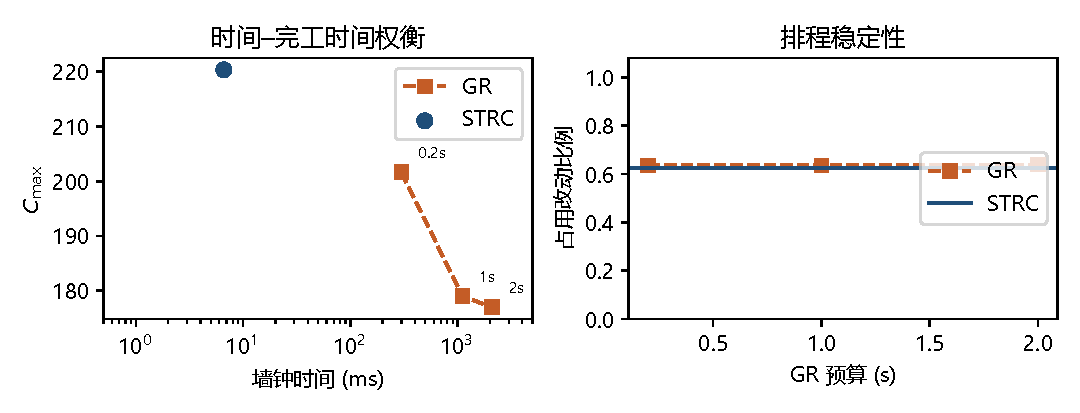
\includegraphics[width=\linewidth]{figures/fig_strc_e5_CN_new}
\caption{E5：不改写已结束占用的 GR 预算扫描与有界修复结果（拥堵例，\(3\) 个随机种子均值）。
左：算法耗时与 \(C_{\max}\)；右：占用改动比例。}
\Description{并排两幅图。左幅横轴为对数刻度的算法耗时、纵轴为完工时间：
不改写已结束占用的热启动全局重调度随预算略降，有界修复是左上方的一个单点，
两者不相交，全局重调度在每个预算点上都略低。右幅为占用改动比例，
两法均约为 0.6。}
\label{fig:e5}
\end{figure}

\begin{table}[t]
\centering
\caption{E5 与不改写已结束占用的热启动全局重调度（\(3\) 个随机种子均值）。
本表只含本文构造的两个算例：\(2\) 算例 \(\times\) \(3\) 随机种子 \(\times\) \(3\) 预算点，独立的算例--随机种子对共 \(6\) 个；
外部布局批次见第~\ref{sec:pubrepro}~节。「改动比例」为被改写的占用占全表之比。
\STRC{} 在每对上只运行一次、不受预算影响，故同一算例三个预算行中的 \STRC{} 两列数值相同，均为同一次运行的结果。}
\label{tab:e5}
\small
\begin{tabular}{@{}lcccc@{}}
\toprule
算例 & 预算/s & GR \(C_{\max}\) & \STRC{} \(C_{\max}\) & 改动比例 GR / \STRC{} \\
\midrule
\multirow{3}{*}{拥堵例}
 & \(0.2\) & \(201.7\) & \(220.3\) & \(0.64\) / \(0.62\) \\
 & \(1.0\) & \(179.0\) & \(220.3\) & \(0.64\) / \(0.62\) \\
 & \(2.0\) & \(177.0\) & \(220.3\) & \(0.64\) / \(0.62\) \\
\addlinespace[2pt]
\multirow{3}{*}{小例}
 & \(0.2\) & \(61.0\)  & \(78.3\)  & \(0.61\) / \(0.57\) \\
 & \(1.0\) & \(60.3\)  & \(78.3\)  & \(0.61\) / \(0.57\) \\
 & \(2.0\) & \(60.3\)  & \(78.3\)  & \(0.61\) / \(0.57\) \\
\bottomrule
\end{tabular}
\end{table}

本文构造的两个算例的结果如表~\ref{tab:e5} 与图~\ref{fig:e5} 所示，从中可以看到四点。

第一，表~\ref{tab:e5} 中每个预算点上 GR 的 \(C_{\max}\) 均值都低于 \STRC{}，图~\ref{fig:e5} 左的两条曲线不相交；
逐个算例--随机种子对计数，连同外部布局批次，\(\EfivePts\) 个预算点上 GR 胜/持平/负为 \(\EfiveWLT\)，
持平与更差的点均在最小预算上：持平的是小例的随机种子 \(42\) 与外部布局 \texttt{L6} 的随机种子 \(2024\)，
更差的一点是外部布局 \texttt{L2} 的随机种子 \(2024\)（GR \(142.5\)、\STRC{} \(141\)；第~\ref{sec:pubrepro}~节）。

第二，所测区间内只在这一对上出现交叉点，且交叉发生在最小预算与 \(1\)\,s 之间。
\STRC{} 的 \(C_{\max}\) 不随预算变化；GR 报告的是逐代最优，随机种子固定后增加预算只是让同一条搜索轨迹多运行若干代，
\(C_{\max}\) 单调不增。因此在最小预算上 GR 已不差于 \STRC{} 的对，增加预算不会使次序反转；
交叉只可能出现在最小预算上 GR 更差的对上，本批中只有上述一对，GR 在 \(1\)\,s 预算时即反超（\(135\) 对 \(141\)）。
在最小预算上，\(\EfiveCells\) 对中 GR 有 \(\EfiveWinMin\) 对严格更优、\(\EfiveTieMin\) 对持平、\(1\) 对更差。
需要说明的是，预算按墙钟时间计，\(0.2\)\,s 内能评估的代数随机器负载浮动：
两次完整重跑之间，该对与外部布局 \texttt{L6} 随机种子 \(7\) 在最小预算上的 GR 结果都有变化，而同一对上 \STRC{} 的结果逐点相同。
因此「最小预算上 GR 不差于 \STRC{}」只是这 \(\EfiveCells\) 对上、单次运行的观测，换用其他算例或机器未必成立。
同一对的三个预算点属于同一条搜索轨迹，彼此不独立，故本节不作显著性检验。

第三，上述推广不适用于更低的预算。GR 每评估一个候选至少要做一次解码；在 E6 的算例上一次解码约需
\(\MsRedecode\)\,ms（中位数），种群为 \(40\) 个个体，仅评估初始种群就需约 \(0.37\)\,s，
与所测最小预算 \(0.2\)\,s 同量级。因此预算低于 \(0.2\)\,s 时，GR 可能连一代都评估不完，次序可能反转，
而 \STRC{} 只需毫秒量级且在全部对上可行；本文未测试这一范围。

第四，有界修复的完工时间在全部预算点上均较差，但算法耗时低两至三个数量级
（\STRC{} \(\MsRepairMed\)\,ms，对比 \(0.2\)--\(2\)\,s 预算，见图~\ref{fig:e5} 左）。
这一耗时差来自一遍分层回放、不重新启动搜索，\emph{并非}来自影响集划界；
第~\ref{sec:cheap}~节（毫秒量级内的对照）以耗时相近的 UR 对照证实了这一点。
两法的占用改动比例都约为 \(0.6\)（表~\ref{tab:e5} 末列与图~\ref{fig:e5} 右）。

\textbf{已结束占用。}上述完工时间比较中，两法都不改写已经结束的占用。GR 采用第~\ref{sec:afault}~节定义的固定前缀解码；
若在 \(t_{\mathrm{now}}\) 时某辆 AGV 已空驶出发去取货，而该工件的前一道工序尚未完工、取货时刻须重新确定，
GR 仍用原 AGV，已驶过的路段原样保留，只重新规划 \(t_{\mathrm{now}}\) 之后的部分。
逐点检查表明，两个算例各 \(9\) 个预算点上 GR 改写已结束占用的次数均为 \(\RzeroPastLo\)，
有界修复在相同的对上同样为零。因此两法的完工时间差距不包含「改写已结束的占用」带来的部分，
而来自全局改派与改序相对一遍分层回放的优势。

结论：要求毫秒量级响应时，有界修复能够恢复可行；允许秒级停机时，不改写已结束占用的热启动全局重调度
在完工时间上占优。预约影响集的作用不体现在完工时间上，其适用场景是要求毫秒量级响应的恢复。

%% 标题里不放 \(\times\):它会进 PDF 书签,hyperref 无法处理数学模式。
\subsubsection{E6：毫秒量级内的对照}
\label{sec:cheap}

E5 的对照是热启动种群搜索，预算 \(0.2\)--\(2\)\,s。仅以它为对照会留下一个问题：
\emph{「低两至三个数量级」这一结果，有多少来自预约影响集，又有多少只是因为对照方法耗时更长?}
本节补充耗时介于有界修复与热启动种群搜索之间的对照，并加入一个仅改变允许改写范围的对照。

三种对照的定义见第~\ref{sec:vs_r0}~节，这里只补充与本节比较有关的两点。
RS 的延迟 \(\Delta\) 取到刚好让受阻走廊上所有可动的占用落到阻断时段之后；由于是统一平移，
两条被平移占用之间的间隔不变，冻结占用与被平移占用之间的间隔只增不减，而优先、机器与走廊约束都是「\(\ge\)」型。
唯一的例外是节点容量：\(t_{\mathrm{now}}\) 时在途的运输可能在 \(t_{\mathrm{now}}\) 之后才到达某节点，
而本应先离开该节点的车被推迟，二者在该节点上重叠；此时校验报错，记为不可行。
UR 与 \STRC{} 使用同一套分层回放程序、面对同一段阻断，只差改写集取 \(W\) 还是全部尚未完成的运输，
因此它是唯一能单独隔离预约影响集作用的对照。E3（只更换划界对象）比较的是两种\emph{不同}的划界对象，
UR 回答的则是：\emph{是否需要按影响集限制改写范围}。

\begin{table}[t]
\centering
\caption{E6 毫秒量级内对照（\(\NPairs\) 对，设置与 E3 相同：繁忙走廊整段阻断，\STRC{} 不做范围扩展）。
可行对数为 RS \(43\)，RD、UR 与 \STRC{} 各 \(\NPairs\)；「平均退化」与「改动比例」按各法自身可行的对计，末列按两法均可行的对计。
「改写已结束占用」计改写了已结束占用的算例--随机种子对；「允许改写」为该方法纳入改写的占用占 \(t_{\mathrm{now}}\)
之后尚未结束占用的比例，\STRC{} 一行按预约影响集 \(\mathrm{Cl}\) 计（按运输补齐后为 \SegShare）；末列为该方法对 \STRC{} 的 \(C_{\max}\) 胜负。
「平均退化」为 \((C_{\max}(\mathcal{S}')-C_{\max}(\mathcal{S}^0))/C_{\max}(\mathcal{S}^0)\) 的均值，其中 \(\mathcal{S}^0\) 为扰动前的排程，\(\mathcal{S}'\) 为修复后的排程。
表~\ref{tab:e5} 只含小例与拥堵例两个算例，与本表的 \(\NPairs\) 对不是同一组算例，故两表数值不宜直接比较。}
\label{tab:cheap}
\small
\begin{tabular}{@{}lcccccc@{}}
\toprule
方法 & 改写已结束占用 & ms（中位）& 平均退化 & 改动比例 & 允许改写 & 对 \STRC{} 赢/平/输 \\
\midrule
RS 全局右移      & \ShiftBad     & \MsShift    & \(56.9\%\) & \ResFracShift    & ---   & \(5/14/24\) \\
RD 重解码        & \RedecodeBad  & \MsRedecode & \(50.2\%\) & \ResFracRedecode & ---   & \(28/13/9\) \\
UR 不按影响集划界 & \ShiftBad     & \MsAllFuture & \(52.4\%\) & \ResFracAllFuture & \(1.00\) & \(0/50/0\) \\
\STRC{} 有界修复      & \ShiftBad     & \MsCheapRtwo & \(52.4\%\) & \ResFracCheapRtwo & \ClosureShareMean & --- \\
\bottomrule
\end{tabular}
\end{table}

结果如表~\ref{tab:cheap} 所示，从中可以看到四点。

其一，RS 只需 \MsShift\,ms，约为 \STRC{} 的四分之一，是各法中唯一比有界修复更快的方法
（按工序依赖图划界的 AOR 更快，但其可行率仅为 \FeasRone，不构成候选方法）。
代价有三：有 \(7\) 对因上述节点容量冲突而不可行；完工时间平均退化 \(56.9\%\)（\STRC{} 为 \(52.4\%\)），逐对比较为 \WinVsShift（\STRC{} 赢/平/输）；
改动的占用更多（\ResFracShift\ 对 \ResFracCheapRtwo），因为统一平移改变了每一条尚未结束占用的时刻。
若要使右移\emph{有选择}，即只推迟真正受影响的 AGV 而其余保持不变，就必须先
确定哪些占用受影响，而这正是本文划定的范围。
\textbf{因此，右移的速度来自放弃选择，代价是可行率、完工时间与改写量都更差。}

其二，RD 的耗时中位数为 \MsRedecode\,ms，是 \STRC{} 的 \RedecodeRatio\ 倍；在第~\ref{sec:instscale}~节的规模序列上，这一倍数随算例增大升至 \(\ScaleRatioHi\)。
这一结果与搜索配置无关：任何基于解码的搜索，每评估一个候选至少需要一次解码。
\textbf{因此，即使换成同一实现中耗时最短的全局重算，有界修复仍不更慢，且算例越大优势越明显}。

其三，两法在全部 \(\NPairs\) 对上均可行，\STRC{} 对 RD 为 \WinVsRedecode（赢/平/输），平均退化 \(52.4\%\) 对 \(50.2\%\)；
逐对取 \STRC{} 的退化减 RD 的退化（正值表示 RD 更优），配对差均值为 \(+0.022\)，
自助 \(95\%\) 区间 \([0.001,\,0.042]\) 不含 \(0\)，Wilcoxon 符号秩双侧 \(p=0.004\)（Holm 校正后 \(0.014\)），RD 的完工时间显著略优。
RD 在全部对上都没有改写已结束的占用（表~\ref{tab:cheap} 第二列为 \RedecodeBad）：若在 \(t_{\mathrm{now}}\) 时某辆 AGV 已空驶出发去取货，而该工件的前一道工序尚未完工，
RD 仍用原 AGV，已驶过的路段原样保留，只重新规划之后的部分。因此 RD 在逐对胜负计数上的优势来自同一染色体下全局改路相对分层回放的优势，
而非改写已结束的占用。RD 的改动比例为 \ResFracRedecode，略高于 \STRC{} 的 \ResFracCheapRtwo。
\textbf{因此，在不改写已结束占用的前提下，RD 的完工时间比 \STRC{} 平均好约 \(2\) 个百分点，代价是耗时为其 \RedecodeRatio\ 倍（规模序列上升至 \ScaleRatioHi\ 倍）、改写略多。}

其四，UR 与 \STRC{} 只差改写集，二者之差就是按影响集划界的收益。在本批次的整段阻断下，这一收益几乎为零：
改写集平均已占全部尚未完成运输的 \(0.963\)，两法完工时间逐对全部相同（\WinVsAllFuture），
改动比例只在 \(3\) 对上不同（\RAStabWTL，\STRC{} 更少/相同/更多），平均差不到 \(0.001\)；
差值非零的对不足 \(6\) 个，不作检验。
耗时上 \STRC{} 略慢（\MsCheapRtwo\ 对 \MsAllFuture\,ms，逐对比值中位数 \(1.11\)），其中在线划界本身的中位数约 \(0.6\)\,ms。

结论：在不改写已结束占用、响应须在毫秒量级的条件下，\STRC{} 与 UR 耗时相近、完工时间相近，
说明毫秒量级的响应来自一遍分层回放、不重新启动搜索，而非来自预约影响集。
同在毫秒量级的对照中，RS 更快但可行率、完工时间与改写量都更差，RD 完工时间略优但更慢、改写略多。
划界的收益在本批次的整段阻断下几乎为零，它随算例规模与阻断时长的变化见第~\ref{sec:ablation}~节。

\subsection{消融：划界与分层}
\label{sec:ablation}

E7 把 \STRC{} 拆成两部分分别检验：按影响集划定改写集 \(W\)（划界），以及在 \(W\) 内分层回放（分层）。
\STRC{} 对 UR 只差划界，UR 对不分层的 RR 只差分层，\STRC{} 对 RR 为二者合计。

\subsubsection{划界：\STRC{} 对 UR}
\label{sec:boundary}

E6（毫秒量级内的对照）的第四点说明，在主批次的五个算例与整段阻断下，影响集几乎覆盖全部尚未完成的运输，划界无从体现。
划界的作用在于让冻结集 \(F\) 保持原值，不被其他运输的重规划挤动；只有当 \(F\) 足够大、且 UR 下 \(F\) 中的占用确实会被挤动时，二者才拉开差距。
为此，在主批次上另把阻断截短为 \(5\) 与 \(2\) 个时间单位，并在第~\ref{sec:instscale}~节的规模序列（\(k=4\)--\(10\)，每个 \(k\) 取 \(\NSeeds\) 个随机种子）上重复三种阻断时长，
其余设置同 E6。这两项是在看到 E6 的结果之后加入的（第~\ref{sec:protocol}~节「统计方法」）。结果如表~\ref{tab:boundary} 所示。

\begin{table}[t]
\centering
\caption{E7 划界收益：\STRC{} 对 UR（同为分层回放、不做范围扩展；只计两法均可行的对）。
\(W/\mathrm{alive}\) 为改写集占尚未完成运输的比例；「UR 改动」为 UR 下被改路或改时刻的运输占尚未完成运输的比例；
\(\Delta\)改动比例为 \STRC{} 减 UR 的改动比例（占全表占用）的均值，负值表示 \STRC{} 改写更少；
「更少/相同/更多」与 \(C_{\max}\) 的「赢/平/输」均站在 \STRC{} 一方；\(p\) 为 Wilcoxon 符号秩双侧检验经 Holm 校正后的值，
差值非零的对不足 \(6\) 时记「---」；\(C_{\max}\) 比与耗时比均为 \STRC{} 除以 UR，前者取均值，后者取逐对比值的中位数。}
\label{tab:boundary}
\small
\setlength{\tabcolsep}{3pt}
\begin{tabular}{@{}llcccccccc@{}}
\toprule
批次 & 阻断 & 对数 & \(W/\mathrm{alive}\) & UR 改动 & \(\Delta\)改动比例 & 更少/相同/更多 & \(p\) & \(C_{\max}\) 比 & 耗时比 \\
\midrule
主批次 & 整段 & \(50\) & \(0.963\) & \(0.897\) & \(-0.000\) & \(2/47/1\) & --- & \(1.000\) & \(1.11\) \\
主批次 & \(L=5\) & \(48\) & \(0.927\) & \(0.737\) & \(-0.018\) & \(7/40/1\) & \(0.26\) & \(1.000\) & \(1.13\) \\
主批次 & \(L=2\) & \(48\) & \(0.917\) & \(0.561\) & \(-0.015\) & \(7/39/2\) & \(0.26\) & \(1.003\) & \(1.11\) \\
\addlinespace[2pt]
规模序列 & 整段 & \(68\) & \(0.898\) & \(0.827\) & \(-0.017\) & \(14/54/0\) & \(0.005\) & \(0.999\) & \(1.05\) \\
规模序列 & \(L=5\) & \(69\) & \(0.845\) & \(0.700\) & \(-0.059\) & \(27/40/2\) & \(6\times10^{-4}\) & \(0.995\) & \(1.04\) \\
规模序列 & \(L=2\) & \(69\) & \(0.820\) & \(0.600\) & \(-0.082\) & \(30/36/3\) & \(1\times10^{-4}\) & \(0.998\) & \(1.03\) \\
\bottomrule
\end{tabular}
\end{table}

从表~\ref{tab:boundary} 可以看到三点。

第一，\textbf{在主批次上，划界的收益很小且不显著}。整段阻断下 \(\Delta\)改动比例几乎为零；
\(L=5\) 与 \(L=2\) 时多数非零的对是 \STRC{} 改写更少（\(7/40/1\) 与 \(7/39/2\)），平均少 \(0.018\) 与 \(0.015\)，但校正后 \(p\) 均为 \(0.26\)。
两种短阻断下 \STRC{} 首轮都只在 \(48\) 对上可行，而 UR 在全部 \(50\) 对上可行：
未恢复的是 \texttt{S11} 与 \texttt{S21} 的随机种子 \(99\)，冻结集里的同一次运输在新排程下早于工件就绪就要取货，预提交即失败；
开启范围扩展后，这几对都在第三级（纳入全部尚未完成的运输）恢复可行（第~\ref{sec:scope_escalation}~节）。
因此，在小规模算例上，划界没有可确认的改写量收益，还会让少数对需要扩大范围。

第二，\textbf{在规模序列上，划界使被改写的占用明显减少，且阻断越短越明显}。
整段阻断时平均少改写全表占用的 \(1.7\) 个百分点，\(L=5\) 与 \(L=2\) 时分别为 \(5.9\) 与 \(8.2\) 个百分点；三者经 Holm 校正后均显著。
原因可从前两列读出：阻断越短，UR 实际改动的运输越少（\(0.83\to0.60\)），而 \(W\) 外的冻结集仍占 \(10\%\)--\(18\%\)；
UR 下冻结集中的运输会被其他运输的重规划挤动，\STRC{} 则把它们原样保留。
逐 \(k\) 看，收益集中在 \(k=8\)、\(9\)：\(L=5\) 与 \(L=2\) 时 \(\Delta\)改动比例为 \(-0.11\)--\(-0.19\)；
\(k=4\) 时只有 \(-0.008\)--\(-0.021\)，与主批次相近。

第三，\textbf{划界不改变完工时间，也不改变耗时}。\(C_{\max}\) 比在 \(0.995\)--\(1.003\) 之间，逐对胜负双向都有；
耗时比在 \(1.03\)--\(1.13\) 之间，其中在线划界在主批次上约 \(0.6\)\,ms、在规模序列上约 \(1.0\)--\(1.1\)\,ms，占 \STRC{} 耗时的 \(7\%\)--\(10\%\)。

\subsubsection{分层：UR 对 RR}
\label{sec:layering}

分层指在 \(W\) 内只让重规划集在全图上搜索、平移集先沿原路线只改时刻。
在上述六组设置上加入不分层、不划界的 RR：UR 对 RR 只差分层，\STRC{} 对 RR 为分层与划界的合计。
结果如表~\ref{tab:ablation} 所示。

\begin{table}[t]
\centering
\caption{E7 分层与划界的消融（只计两法均可行的对）。「可行」为 RR/UR/\STRC{} 的首轮可行对数；
\(\Delta\)改动比例与 \(C_{\max}\) 变化均取前者减后者的均值，后者以百分比计；耗时比取逐对比值（前者除以后者）的中位数；
\(p\) 为 UR 对 RR 耗时差（逐对比值取对数）的 Wilcoxon 符号秩双侧检验经 Holm 校正后的值。划界一项见表~\ref{tab:boundary}。}
\label{tab:ablation}
\small
\setlength{\tabcolsep}{3pt}
\begin{tabular}{@{}llccccccccc@{}}
\toprule
 & & & \multicolumn{4}{c}{分层：UR 对 RR} & \multicolumn{3}{c}{合计：\STRC{} 对 RR} \\
\cmidrule(lr){4-7}\cmidrule(l){8-10}
批次 & 阻断 & 可行 & \(\Delta\)改动比例 & \(C_{\max}\) 变化 & 耗时比 & \(p\) & \(\Delta\)改动比例 & \(C_{\max}\) 变化 & 耗时比 \\
\midrule
主批次 & 整段 & \(50/50/50\) & \(+0.000\) & \(+0.05\%\) & \(0.99\) & \(1.00\) & \(-0.000\) & \(+0.05\%\) & \(1.11\) \\
主批次 & \(L=5\) & \(50/50/48\) & \(+0.002\) & \(+0.7\%\) & \(0.92\) & \(3\times10^{-5}\) & \(-0.016\) & \(+0.7\%\) & \(1.05\) \\
主批次 & \(L=2\) & \(50/50/48\) & \(+0.003\) & \(+0.4\%\) & \(0.90\) & \(2\times10^{-5}\) & \(-0.013\) & \(+0.6\%\) & \(0.98\) \\
\addlinespace[2pt]
规模序列 & 整段 & \(68/68/68\) & \(+0.006\) & \(+1.8\%\) & \(0.90\) & \(9\times10^{-8}\) & \(-0.011\) & \(+1.7\%\) & \(0.96\) \\
规模序列 & \(L=5\) & \(68/69/69\) & \(+0.015\) & \(+3.2\%\) & \(0.84\) & \(<10^{-10}\) & \(-0.045\) & \(+2.6\%\) & \(0.87\) \\
规模序列 & \(L=2\) & \(69/70/69\) & \(+0.010\) & \(+2.4\%\) & \(0.83\) & \(1\times10^{-10}\) & \(-0.073\) & \(+2.1\%\) & \(0.84\) \\
\bottomrule
\end{tabular}
\end{table}

从表~\ref{tab:ablation} 可以看到三点。

第一，\textbf{分层的贡献在耗时}。除主批次整段阻断外（耗时比 \(0.99\)，无差别），UR 比 RR 快 \(8\%\)--\(17\%\)，经 Holm 校正后均显著；
阻断越短、算例越大，加速越明显，因为此时重规划集只占 \(W\) 的一小部分（第~\ref{sec:level1}~节），其余运输只在原路线的子图上搜索。
分层并不减少改动：平移集沿原路线只改时刻，同样计为改动，故改动比例与 RR 相当或略高（\(+0.000\)--\(+0.015\)）；
它也让完工时间略差（\(+0.05\%\)--\(+3.2\%\)），因为平移集的运输不再寻找更短的路线。首轮可行对数与 RR 相同或多 \(1\) 对。

第二，\textbf{划界的贡献在改写量}（表~\ref{tab:boundary}）：在规模序列上使改动比例降低 \(0.017\)--\(0.082\)，不改变完工时间，耗时略增 \(3\%\)--\(5\%\)。

第三，\textbf{二者合计}，在规模序列上 \STRC{} 比 RR 少改写全表占用的 \(1.1\)--\(7.3\) 个百分点，还快 \(4\%\)--\(16\%\)，代价是完工时间增加 \(1.7\%\)--\(2.6\%\)；
在主批次上，合计改动比例比 RR 低 \(0.000\)--\(0.016\)，完工时间增加 \(0.05\%\)--\(0.7\%\)，耗时相当（耗时比 \(0.98\)--\(1.11\)）。
可见分层与划界各管一头：前者换取速度，后者换取冻结集的稳定，二者都以少量完工时间为代价，且只在算例较大时有可见的收益。

结论：\textbf{按影响集划界的收益体现在改写量上，且只在冻结集足够大时出现}：
在本批次的五个小规模算例上很小且不显著，在较大的算例与较短的阻断下，被改写的占用占全表的比例平均降低 \(2\)--\(8\) 个百分点，
因为影响集外的占用按命题~\ref{prop:outside} 保持原计划，不随其他运输的重规划移动。
分层则贡献耗时上的 \(8\%\)--\(17\%\)（主批次整段阻断下无差别），不减少改写。
若允许秒级耗时，GR 能得到更短的完工时间（第~\ref{sec:e5}~节）。

\subsection{规模外推}
\label{sec:e8}

本节（E8）从两个方向扩大规模，检验有界修复是否仍能恢复可行、耗时是否仍在毫秒量级：
先在固定算例上扩大扰动规模，再在固定扰动设置下扩大算例本身。两部分均启用范围扩展。

\subsubsection{扰动规模}
\label{sec:scale}

本部分检验：扰动规模增大时，有界修复是否仍能恢复可行，耗时是否仍在毫秒量级。
算例为拥堵例与小例，各 \(\NSeeds\) 个随机种子；受扰工序比例 \(\varphi\) 取 \(0.10\)、\(0.25\)、\(0.50\)、\(0.75\)、\(1.00\)，
\(\varphi=1\) 表示 \(t_{\mathrm{now}}\) 之后的全部工序都受扰动。
与 E3（只更换划界对象）、E5（与全局重调度对比）不同，这里的有界修复启用范围扩展；GR 预算为 \(2\)\,s。

\begin{table}[t]
\centering
\caption{E8 扰动规模扫描（拥堵例，\(\NSeeds\) 个随机种子平均；有界修复启用范围扩展；GR 预算 \(2\)\,s）。
「触发扩展」计首轮分层回放失败、进入范围扩展的对数。
有界修复在各对上的耗时为 \ScaleMsMin--\ScaleMsMax\,ms；\(C_{\max}\) 在各 \(\varphi\) 取值上的四分位距，有界修复为 \(8\)--\(17\)，GR 为 \ScaleCmaxIqrLo--\ScaleCmaxIqrHi。
扰动前原排程的 \(C_{\max}\) 均值为 \(139.4\)。}
\label{tab:scale}
\small
\begin{tabular}{@{}rccccc@{}}
\toprule
\(\varphi\) & 有界修复可行 & 触发扩展 & 有界修复 ms & 有界修复 \(C_{\max}\) & GR \(C_{\max}\) \\
\midrule
\(0.10\) & \(100\%\) & \(1/10\) & \(6.2\) & \(148.9\) & \(129.1\) \\
\(0.25\) & \(100\%\) & \(1/10\) & \(6.6\) & \(165.3\) & \(142.7\) \\
\(0.50\) & \(100\%\) & \(0/10\) & \(6.8\) & \(178.4\) & \(156.6\) \\
\(0.75\) & \(100\%\) & \(0/10\) & \(7.6\) & \(196.1\) & \(159.7\) \\
\(1.00\) & \(100\%\) & \(0/10\) & \(8.1\) & \(202.6\) & \(172.4\) \\
\bottomrule
\end{tabular}
\end{table}

\begin{figure}[tbp]
\centering
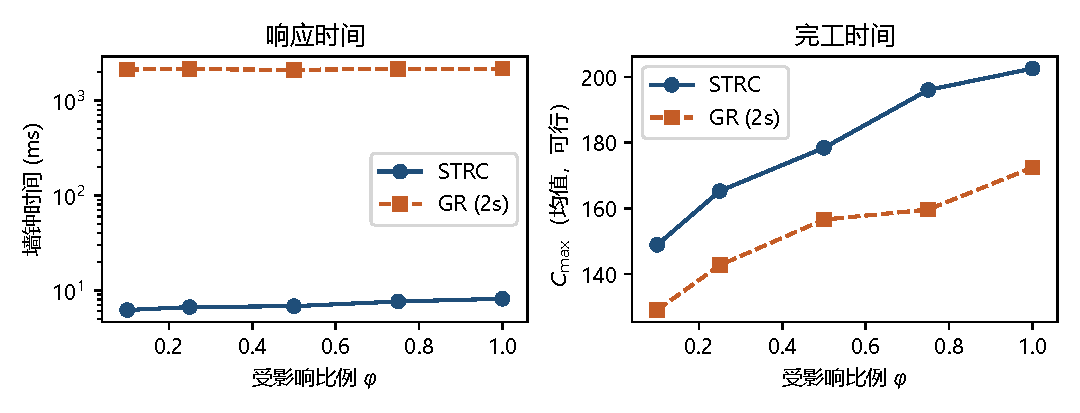
\includegraphics[width=\linewidth]{figures/fig_strc_scale_CN_new}
\caption{E8 扰动规模扫描（拥堵例，\(\NSeeds\) 个随机种子）：
有界修复与 GR 的算法耗时（对数轴）与完工时间随 \(\varphi\) 变化。曲线取各 \(\varphi\) 取值上的均值，
离散度的度量与表~\ref{tab:scale} 相同（四分位距）。}
\Description{两条随扰动比例变化的曲线。算法耗时画在对数纵轴上：有界修复始终在
十毫秒量级、随比例上升只略有增长，全局重调度固定在两秒的预算线上。完工时间一侧，
全局重调度随扰动比例增大而缓慢上升，但始终低于有界修复。}
\label{fig:scale}
\end{figure}

拥堵例的结果如表~\ref{tab:scale} 与图~\ref{fig:scale} 所示，从中可以看到四点。
第一，五个 \(\varphi\) 取值下有界修复在每一对上都恢复可行。拥堵例在 \(\varphi=0.10\) 与 \(0.25\) 时各有 \(1\) 对（随机种子 \(7\) 与 \(2024\)）首轮失败，
经范围扩展在第三级恢复，其余各对都首轮可行；小例上全部首轮可行。
第二，本部分检验的是可行性与耗时，\emph{不}检验划界的收益：受扰工序沿工件链牵连其后的全部运输，
拥堵例在各 \(\varphi\) 取值上改写集都已约等于全部尚未完成的运输，此时有界修复与 UR 的改写集合相同。
小例在 \(\varphi=0.10\) 时有 \(5\) 对改写集为空，其余取值同样接近全部。
第三，有界修复的耗时随 \(\varphi\) 只缓慢上升：拥堵例在各 \(\varphi\) 取值上的均值为 \(6.2\)--\(8.1\)\,ms（含范围扩展），
各对为 \ScaleMsMin--\ScaleMsMax\,ms；小例为 \(1.1\)--\(1.9\)\,ms。
第四，GR 在拥堵例每个 \(\varphi\) 取值的每一对上 \(C_{\max}\) 都更优，小例上胜 \(8\)--\(10\) 对、其余持平，与 E5 一致，但它用满 \(2\)\,s 预算，耗时高两至三个数量级。
\(\varphi=0.10\) 时 GR 的 \(C_{\max}\) 均值（\(129.1\)）低于扰动前原排程的 \(139.4\)，\(\varphi=0.25\) 时也有一半的对低于各自的原排程：
原排程按启发式构造、未经优化（第~\ref{sec:protocol}~节），
GR 可同时改机器指派与加工顺序，所以它在恢复的同时也优化了原排程；有界修复保持指派与顺序不变，\(C_{\max}\) 只能在原排程之上增加
（\(148.9\)--\(202.6\)）。两者的完工时间差因此不只是修复能力之差。

结论：在所测扰动规模内，有界修复始终恢复可行（两个算例、五个 \(\varphi\) 取值共 \(100\) 次运行中，\(2\) 次需要范围扩展），耗时保持在十毫秒量级，随扰动规模只缓慢增长；
扰动规模较大时影响集接近全部尚未完成的运输，本部分不反映划界的收益。

\subsubsection{算例规模}
\label{sec:instscale}

上一部分扫描的是\emph{扰动}的规模，算例始终为 \(8\) 工件 \(4\) 机。本部分固定扰动设置、扩大算例本身，
检验算例规模增大时，影响集占比是否随之接近 \(1\)、使「有界」失去实际意义，同时记录耗时的变化。

规模序列取工件数 \(2k\)、机器数 \(k\)、AGV 数 \(k\)（\(k=4,\dots,10\)），即 \(8\times4\times4\) 到
\(\ScaleJobsHi\times\ScaleMachHi\times\ScaleMachHi\)，共 \(\ScaleKs\) 个规模 \(\times\)
\(\NSeeds\) 个随机种子 \(=\ScalePairs\) 对。拥堵等级、异构度、柔性度、运输/加工时长比与毛坯库
最小割、远端割全部按同一目标标定，\emph{只改变规模}。三个对照方法与第~\ref{sec:cheap}~节定义相同。
每个规模的算例均由同一随机种子 \(42\) 生成，只有一个拥堵等级；E4（四类扰动下的划界与修复）与 E8 的扰动规模部分未在这批算例上重新运行；E7（划界与分层的消融）用的是这批算例（第~\ref{sec:ablation}~节）。

\begin{table}[t]
\centering
\caption{E8 算例规模扫描（\(\ScaleKs\) 个规模 \(\times\) \(\NSeeds\) 个随机种子）。
「影响集」为预约影响集占\emph{全表}之比，该比的可达上界是 \(|R^{\circ}|/|R|\)、本批均值约
\ScaleAliveShare；换以可改写集合为分母则为 \ScaleCloAliveLo--\ScaleCloAliveHi（见正文）。
耗时取中位数，「RD/\STRC{}」一列即两列\emph{中位数之比}；正文讨论其单调性时用的是先在每对上求比值、
再按规模平均的结果，两种计算方式下各规模的起落一致但数值不同。
末两列为 RS 的可行对数，以及在两法均可行的对上 \STRC{} 对 RS 的 \(C_{\max}\) 胜负。}
\label{tab:instscale}
\small
\begin{tabular}{@{}lrcccccc@{}}
\toprule
规模 & \(|R|\) & 影响集 & \STRC{}\,ms & RD\,ms & RD/\STRC{} & RS 可行 & \STRC{} 对 RS \\
\midrule
\(8\times4\times4\)    & \(161\) & \(0.568\) & \(7.7\)  & \(9.0\)  & \(1.2\times\) & \(8\) & \(6/1/1\) \\
\(10\times5\times5\)   & \(193\) & \(0.531\) & \(9.0\)  & \(12.4\) & \(1.4\times\) & \(4\) & \(3/0/1\) \\
\(12\times6\times6\)   & \(252\) & \(0.559\) & \(12.8\) & \(20.4\) & \(1.6\times\) & \(3\) & \(2/0/1\) \\
\(14\times7\times7\)   & \(304\) & \(0.548\) & \(16.5\) & \(29.8\) & \(1.8\times\) & \(8\) & \(3/0/4\) \\
\(16\times8\times8\)   & \(328\) & \(0.509\) & \(19.5\) & \(37.5\) & \(1.9\times\) & \(2\) & \(2/0/0\) \\
\(18\times9\times9\)   & \(386\) & \(0.515\) & \(22.1\) & \(47.9\) & \(2.2\times\) & \(3\) & \(3/0/0\) \\
\(20\times10\times10\) & \(438\) & \(0.535\) & \(26.3\) & \(79.8\) & \(3.0\times\) & \(4\) & \(4/0/0\) \\
\bottomrule
\end{tabular}
\end{table}

结果如表~\ref{tab:instscale} 所示，从中可以看到四点。

第一，七个规模上 \(\mathrm{Cl}/|R|\) 在 \ScaleCloLo--\ScaleCloHi 之间波动，且不单调
（\(k=4,6\) 最高，\(k=8,9\) 最低），没有上升趋势。由于 \(\mathrm{Cl}\) 只包含
\(t_{\mathrm{now}}\) 之后尚未结束的占用，而本批尚未结束的占用只占全表约 \ScaleAliveShare，
\(\mathrm{Cl}/|R|\) 最多只能到约 \ScaleAliveShare，用它判断是否接近 \(1\) 没有意义。
换用尚未结束的占用作分母后，七个规模上 \(\mathrm{Cl}/|R^{\circ}|\) 都在 \ScaleCloAliveLo--\ScaleCloAliveHi 之间
（最小规模为 \(0.91\)，最大规模为 \(0.90\)，\(k=9\) 最低，为 \(0.82\)），与 E4、E6（毫秒量级内的对照）中的 \ClosureAliveFrac\ 同量级。
因此，影响集占比没有随算例规模增大而上升；它覆盖尚未结束占用的 \(82\%\)--\(92\%\)，冻结集只占其余一小部分，
而正是这一部分在 E7 中带来了改写量上的差别（第~\ref{sec:boundary}~节）。

第二，\(|R|\) 增至 \(2.7\) 倍时，\STRC{} 的耗时中位数从 \(7.7\)\,ms 增至 \ScaleMsHi\,ms，即 \(3.4\) 倍，
仍在十毫秒量级；七个规模的数据不足以判断耗时随规模增长的快慢。首轮分层回放（不做范围扩展）即在 \ScaleFeasFirst\ 对上可行。
首轮失败的 \(2\) 对（\(14\times7\times7\) 的随机种子 \(31415\) 与 \(18\times9\times9\) 的随机种子 \(7\)）经范围扩展到全部尚未完成的运输仍不可行，
UR 与 RR 在这 \(2\) 对上同样失败，失败来自分层回放本身而非 \(W\) 过小；
RD 在这 \(2\) 对上都可行，说明排程本身可以恢复，失败在于逐车依次规划的回放找不到解。最终在 \ScaleFeasAll\ 对上可行。

第三，耗时最短的全局重算 RD 与 \STRC{} 的耗时比从 \ScaleRatioLo\(\times\) 升至 \ScaleRatioHi\(\times\)。
先在每对上求比值再按规模平均，依次为 \(1.12\)、\(1.41\)、\(1.52\)、\(1.79\)、\(1.99\)、\(2.12\)、\(3.00\)，随规模单调上升；
两端相差约 \(1.9\)，大于任一规模内不超过 \(0.59\) 的四分位距。因此，规模越大，有界修复相对全局重算的耗时优势越明显。

第四，全局右移多数情况下不可行：RS 在七个规模上分别有 \(8\)、\(4\)、\(3\)、\(8\)、\(2\)、\(3\)、\(4\) 对可行，共 \(32/\ScalePairs\)，
不可行均来自第~\ref{sec:cheap}~节所述的节点容量冲突；可行率不随规模单调变化，但 \(k\ge8\) 时每个规模都不超过 \(4\) 对。
在两法均可行的 \(31\) 对上，\STRC{} 的 \(C_{\max}\) 胜/平/负为 \(23/1/7\)。

结论：七个规模的数据虽不足以推断更大规模下的趋势，但在 \(8\times4\times4\) 至 \(\ScaleJobsHi\times\ScaleMachHi\times\ScaleMachHi\) 的范围内，
影响集占比没有随算例规模上升，\STRC{} 耗时仍在十毫秒量级，相对全局重算的耗时优势随规模扩大，而全局右移在多数对上不可行。

\subsection{外部布局：复现与结构指标}
\label{sec:pub}

\subsubsection{复现 E1--E3 与 E5}
\label{sec:pubrepro}

本小节检验 E1（工序依赖图给出空范围）、E2（闭合性与集外不变）、E3（只更换划界对象）与 E5（与全局重调度对比）的结论是否依赖本文构造的布局。设置：换用 Lyu 等发表的布局 \texttt{L2}--\texttt{L6}
（第~\ref{sec:protocol}~节「外部布局批次」），每张布局 \(\NSeeds\) 个随机种子，共 \(\NPubPairs\) 对，
其余设置分别与 E1--E3、E5 相同；E5 只在 \texttt{L2} 与 \texttt{L6} 上运行，随机种子 \(\{42,7,2024\}\)、
预算 \(\{0.2,1,2\}\)\,s，共 \(18\) 个预算点。

结果与主批次逐项对应。
E1：\PubPassMiss\ 对上工序依赖图给出空范围，而原排程已不可行。
E2：影响集对依赖边封闭（\PubPassClosed），集外占用逐条不变（\PubPassInvar）。
E3：AOR 可行 \PubFeasRone，\STRC{} 可行 \PubFeasRtwo。
影响集占比：按 E1 的统计方式，各布局 \(\mathrm{Cl}/|R|\) 的中位数为 \PubEoneFracLo--\PubEoneFracHi，
主批次 \(\NPairs\) 对合并的中位数为 \EoneFracMed；外部布局批次略低，两者都约为一半。
E5：\(18\) 个预算点中 \PubEfiveNoCross\ 点 GR 的 \(C_{\max}\) 更优，\(1\) 点持平（\texttt{L6}，随机种子 \(2024\)，预算 \(0.2\)\,s），
\(1\) 点更差（\texttt{L2}，随机种子 \(2024\)，预算 \(0.2\)\,s，GR 在 \(1\)\,s 时反超）；这些点已并入第~\ref{sec:e5}~节的合并统计。

结论：换用已发表的布局后，E1、E2、E3 的结论不变，E5 中 GR 仍在绝大多数预算点上更优；关于划界对象的结论不依赖本文构造的布局。

\subsubsection{E9：路网结构指标能否预测影响集规模（探索性）}
\label{sec:e4}

本节检验：只由路网算出、不随当前排程变化的指标，能否预测预约影响集的规模。考察三个指标：
其一，\emph{LU 割}，即使毛坯库 \(v_{\mathrm{in}}\) 与全部机器断开所需切断的最少走廊数（\(v_{\mathrm{in}}\) 最小割）；
其二，\emph{漏斗占比}，即从 \(v_{\mathrm{in}}\) 到各台机器的最短路中，所有路径都必须经过的走廊，其通行时间占平均路程时间的比例；
其三，每节点走廊数，即走廊数与节点数之比。下文把这三个指标统称为\emph{静态路网指标}。
本节的扰动是阻断 LU 割中的一条走廊，其余设置同第~\ref{sec:protocol}~节；
两批算例共 \(8\) 张布局，每张布局 \(\NSeeds\) 个随机种子。结果如表~\ref{tab:e4pub} 所示。

从表~\ref{tab:e4pub} 最后三行可以看到，本文构造的三张脊式布局的影响集占比在 \SelfCloLo--\SelfCloHi 之间，极差只有 \SelfCloSpread；
而它们的几何差异也很小（节点 \(9\)--\(11\) 个、走廊 \(8\)--\(12\) 条，LU 割只取 \(1\) 或 \(2\)）。
「指标太粗、反映不出布局差异」与「这几张布局本身差别太小」两种解释都与此相符，
\textbf{因此仅凭本文构造的三张布局无法判断静态路网指标是否有效}，需要借助外部布局批次。

外部布局批次的五张布局只落在两张网格上（第~\ref{sec:protocol}~节），所以只能用于考察机器配置这一维。
在同一张 \(4\times 4\) 网格上，只把机器从 \(4\) 台换成 \(5\) 台（\texttt{L2} 换成 \texttt{L3}），
影响集占比的中位数就由 \PubCloHi\ 降到 \PubCloLo，相差 \PubCloSpread；
在同一张 \(5\times 5\) 网格上换三种机器配置（\texttt{L4}--\texttt{L6}），相差 \PubCloSpreadBig。
而本文构造的三张布局路网各不相同，彼此只相差 \SelfCloSpread；前两者约为它的两倍与一点四倍。
这一比较并不对称：Lyu 等的布局同时改变了机器台数与位置，本文的三张布局只改变路网，且彼此几何差异很小，
\SelfCloSpread\ 只是更换路网所引起变化的下界，故不能据此说机器配置的影响大于路网几何。
\textbf{因此，路网不变、只改机器配置，影响集占比就会发生明显变化，机器配置这一维不可忽略。}

表中五个外部算例的 LU 割都是 \(2\)、漏斗占比都是 \(0\)。
原因是两张网格都把毛坯库 \(v_{\mathrm{in}}\) 放在网格角点（图~\ref{fig:layouts}(d)--(h)）：在只允许上下左右移动的网格上，角点只有两条走廊，故 LU 割固定为 \(2\)；
\(v_{\mathrm{in}}\) 到各台机器的最短路也不共用任何一条走廊，故漏斗占比为 \(0\)。
van Os 工具集中的 Liu 2023 布局（因允许对角移动未纳入本批）把装卸点放在网格边的中点，出边数为 \(3\)。
可见 LU 割在实际布局上只取少数几个由 \(v_{\mathrm{in}}\) 位置决定的值，不随路网几何连续变化。
影响集占比在这些算例上变化了 \PubCloSpread，而这两个指标取值不变，故无法解释这一变化。
第三个指标（每节点走廊数）在整批上只取两个值（\(23/16\) 与 \(38/25\)），同样无法解释同一张网格内的变化。
这些指标原本针对脊式布局中可调的毛坯库出口瓶颈而设计，在实际布局上退化为常量。
\textbf{因此，静态路网指标在 Lyu 等的布局上取值恒定，无法解释影响集规模的变化。}

结论：在外部布局批次的 \NPubInst\ 个算例与本文构造的三张布局上，静态路网指标都不能解释影响集规模；
影响集规模更可能取决于运输需求在路网上的空间分布，而不是路网能提供多少条通路，
具体的候选量见第~\ref{sec:limitations}~节「局限与未来工作」第 (2) 条。

\begin{table}[t]
\centering
\caption{E9 静态路网指标与预约影响集占比（阻断 LU 割中的一条走廊；每张布局 \(\NSeeds\) 个随机种子，\(\mathrm{Cl}/|R|\) 取中位数）。
全部算例的工件数、AGV 数与其余生成参数相同，只差路网与机器配置。「节点/走廊」为节点数与走廊数。
「极差」为同一组内各布局影响集占比的最大值减最小值；\(4\times 4\) 网格一组只有 \(2\) 张布局、本文构造的一组只有 \(3\) 张，
故极差只作粗略比较。}
\label{tab:e4pub}
\small
\begin{tabular}{@{}llcccccc@{}}
\toprule
来源与网格 & 布局 & 机器 & 节点/走廊 & LU 割 & 漏斗占比 & \(\mathrm{Cl}/|R|\)
 & 极差 \\
\midrule
Lyu 等，\(4\times 4\) 网格 & \texttt{L2} & \(4\) & \(16/23\) & \(2\) & \(0\) & \(0.552\) & \\
Lyu 等，\(4\times 4\) 网格 & \texttt{L3} & \(5\) & \(16/23\) & \(2\) & \(0\) & \(0.388\)
  & \(\PubCloSpread\) \\
\cmidrule{1-8}
Lyu 等，\(5\times 5\) 网格 & \texttt{L4} & \(6\) & \(25/38\) & \(2\) & \(0\) & \(0.493\) & \\
Lyu 等，\(5\times 5\) 网格 & \texttt{L5} & \(7\) & \(25/38\) & \(2\) & \(0\) & \(0.521\) & \\
Lyu 等，\(5\times 5\) 网格 & \texttt{L6} & \(8\) & \(25/38\) & \(2\) & \(0\) & \(0.420\)
  & \(\PubCloSpreadBig\) \\
\midrule
本文构造 & \texttt{S11} & \(4\) & \(9/8\) & \(1\) & \(0.286\) & \(0.512\) & \\
本文构造 & \texttt{S21} & \(4\) & \(10/10\) & \(2\) & \(0.286\) & \(0.539\) & \\
本文构造 & \texttt{S22} & \(4\) & \(11/12\) & \(2\) & \(0.286\) & \(0.466\)
  & \(\SelfCloSpread\) \\
\bottomrule
\end{tabular}
\end{table}

%% =====================================================================
\section{结论}
\label{sec:conclusion}
%% =====================================================================

\subsection{工作总结}

本文针对用预约表保证 AGV 无冲突通行的柔性作业车间，研究执行期扰动后重调度范围应划定在哪类对象上。
走廊阻断、通行变慢等扰动不改变任何工序的指派与可执行性，却会使走廊占用失效，并沿让行关系传播到其他 AGV。
为此，本文在走廊占用层上划界：提出时空预约闭包（\STRC{}），从受扰占用出发，沿让行、同车、同工件、同机四类依赖边
收集预约影响集；集外占用原样预提交，集内走廊起点所属的运输在全图上重规划，其余运输先沿原路线只改时刻，
仍不可行时先放宽搜索、再逐级扩大允许改写的范围。

让行关系、集内重写而集外保持原计划、失败后扩大允许改写的范围均沿用既有文献（第~\ref{sec:rw_claim}~节）；
本文的主张在于划界对象：工序依赖图按定义不含走廊占用之间的让行关系，因而无法刻画只使占用失效的扰动，
而在预约依赖图上划界后，须改写的占用由既定依赖关系唯一确定，并可在毫秒量级内完成局部恢复。
完工时间上，允许秒级搜索时，热启动全局重调度能得到比有界修复更短的 \(C_{\max}\)。

\subsection{主要结论}

\textbf{(1) 按工序依赖图划界会漏掉一类失效。}
走廊阻断下，在 \(\PassMiss\) 对上按受影响工序划出的范围为空，而原排程确已不可行（第~\ref{sec:e1}~节）；
四类扰动中，B 类扰动均如此（第~\ref{sec:e6}~节）。

\textbf{(2) 预约影响集唯一确定、对外封闭，修复后集外占用保持原计划。}
预约影响集对依赖边封闭（\(\PassClosed\)），修复后集外占用逐条保持原值（\(\PassInvar\)，第~\ref{sec:e2}~节）；
A 类扰动下，预约影响集包含按工序依赖图划出的范围（第~\ref{sec:e6}~节）；
换用 Lyu 等发表的布局后，上述结论不变（第~\ref{sec:pubrepro}~节）。

\textbf{(3) 只更换划界对象即可恢复可行，且耗时为毫秒量级。}
同一套分层回放程序只更换划界对象，可继续执行的排程由 \(\FeasRone\) 变为 \(\FeasRtwo\)（第~\ref{sec:e3}~节），
按工序依赖图划界的失败来自它判定无需重调度、未改动任何占用，而非回放程序的能力不足。有界修复的耗时比热启动全局重调度低两到三个数量级（第~\ref{sec:e5}~节），
与本实现中耗时最短的全局重算 RD 相比也不更慢（\MsCheapRtwo\ 对 \MsRedecode\,ms，第~\ref{sec:cheap}~节），且算例越大优势越明显（耗时比 \ScaleRatioLo--\ScaleRatioHi 倍）；
受扰工序比例增至 \(1\) 时全部恢复可行（\(100\) 次运行中 \(2\) 次需要范围扩展）；算例扩大到 \(\ScaleJobsHi\) 工件 \(\ScaleMachHi\) 机时在 \ScaleFeasAll\ 对上可行，
未恢复的 \(2\) 对 UR 也无法恢复；耗时保持在十毫秒量级（第~\ref{sec:e8}~节）。

\textbf{(4) 按影响集划界的收益体现在改写量上，且只在冻结集足够大时出现。}
与改写全部尚未完成运输的 UR 相比，二者耗时相近、完工时间相近；
在主批次的五个小规模算例上，影响集几乎覆盖全部尚未完成的运输，改写量的差别很小且不显著；
在规模序列上，被改写的占用占全表的比例平均降低 \(1.7\)（整段阻断）至 \(8.2\)（阻断 \(2\) 个时间单位）个百分点，经 Holm 校正后均显著，
来源是冻结集不被其他运输的重规划挤动（第~\ref{sec:boundary}~节）。
消融表明，分层另使耗时减少 \(8\%\)--\(17\%\)（主批次整段阻断下无差别），但不减少改写，且使完工时间略增（第~\ref{sec:layering}~节）。
完工时间上，热启动全局重调度在 \(\EfivePts\) 个预算点中只有 \(1\) 点差于有界修复（第~\ref{sec:e5}~节），耗时相近的 RD 也平均好约 \(2\) 个百分点（第~\ref{sec:cheap}~节）。

\subsection{局限与未来工作}
\label{sec:limitations}

\textbf{(1) 有界修复的完工时间长于全局重算。}
在所测的 \(\EfiveCells\) 个算例--随机种子对上，除一对在最小预算下的情形外，热启动全局重调度在所有预算下都得到更短的 \(C_{\max}\)（第~\ref{sec:e5}~节）；
同在毫秒量级的 RD 也平均短约 \(2\) 个百分点（第~\ref{sec:cheap}~节）。
有界修复虽能在毫秒量级内响应，但只改写影响集内运输的路线与时刻，因而多数情况下完工时间更长。
未来工作可在不改写已结束占用的前提下引入有限度的改派或改序，在完工时间与改写范围之间折中。

\textbf{(2) 影响集的规模取决于算例，目前无法事前预测。}
影响集的大小由占用之间的耦合程度决定：在主批次的紧凑布局上整段阻断时，尚未结束的占用几乎都受到波及，划界减少的改写量有限；
在规模序列上，被改写的占用占全表的比例降低 \(1.7\)--\(8.2\) 个百分点，经 Holm 校正后均显著（第~\ref{sec:boundary}~节）。
只由路网算出的静态指标无法预测这一规模（第~\ref{sec:e4}~节），何时划界有收益目前只能事后判断。
此外，依赖边是按已知的冲突情形逐类构造的，是否涵盖占用之间全部的传播途径，目前尚无证明。
未来工作需以其他扰动形态（例如缩短占用，或延后超过 \(1\) 个时间单位）检验依赖边集的完备性；
在固定修复能力下定义最小允许改写集合，度量影响集与之的差距；
并由随排程而变的量（例如 \(t_{\mathrm{now}}\) 附近受扰走廊上相互重叠的占用条数）预测影响集的规模。

\textbf{(3) 连续扰动与其他路径规划算法尚未检验。}
本文对每次扰动在完整观测后响应一次（假设 A3）；后一次扰动到达时，可以把上一次修复后的排程作为原排程再次划界与修复，
但连续扰动下影响集是否逐次累积变大，未作实验检验；扰动信息有误差、须随新信息反复调整的情形也未建模。
路径规划只采用安全区间规划，其他逐车规划算法未作比较；
规模实验只覆盖到 \(\ScaleJobsHi\) 工件 \(\ScaleMachHi\) 机，依赖图中纳入全部节点停留的做法也未作比较。
未来工作需在连续扰动下检验影响集的规模与分层回放所需的全图搜索次数，并在更大规模与其他路径规划算法上检验。

\textbf{(4) 缺少同时发布路网与运输时间的公开算例。}
现有公开算例族~\cite{homayouni2021production,fontes2023hybrid} 只发布机器之间的运输时间矩阵（每对机器之间一个常数），不包含路网；
由这些矩阵也推不出一张路网，使图上机器之间的最短行程时间与矩阵中的数值一致，因而无法在其上定义走廊占用与走廊阻断。
Lyu 等~\cite{lyu2019approach} 发表了路网，但未给出每条走廊的通行时间；本文借用其路网时按所有走廊等权补齐，
由于通行时间与原文不同，所得数值与 Lyu 或 van Os~\cite{vanos2026exact} 报告的结果没有可比性。
未来工作可在同时发布路网与逐段运输时间的算例上，重复本文关于重调度范围、恢复可行率与全局重调度对比的实验（E1--E3 与 E5）。

\bibliographystyle{ACM-Reference-Format}
\bibliography{reference-base}

\end{document}
